% Electronics 2026 — manuscript draft (portable article layout).
% Port to the MDPI class (mdpi.cls, "electronics" journal option) at submission:
% section files are class-agnostic; only this preamble changes.
\documentclass[10pt,a4paper]{article}
\usepackage[margin=2.5cm]{geometry}
\usepackage[T1]{fontenc}
\usepackage[utf8]{inputenc}
\usepackage{graphicx}
\usepackage{amsmath}
\usepackage{amssymb}
\usepackage{booktabs}
\usepackage{multirow}
\usepackage{xcolor}
\usepackage[colorlinks=true,linkcolor=blue,citecolor=blue]{hyperref}
\usepackage{enumitem}
\setlist{nosep}

\graphicspath{{../figs/}}

\title{From Terrestrial Laser Scans to Queryable Robot Knowledge:\\
A VLM-Verified Framework for Incremental 3D Semantic Modeling}

\author{Sangmin Kim$^{1,2}$ \and Haryeong Kim$^{1}$ \and
Tae-Yong Kuc$^{1,2,*}$\\[2pt]
\small $^1$Department of Electrical and Computer Engineering, Sungkyunkwan University\\
\small $^2$CASELAB Co., Ltd., Anyang \quad $^*$Corresponding author}
\date{Draft \today\ --- not for distribution}

\begin{document}
\maketitle

\begin{abstract}
Indoor service and inspection robots need environment knowledge that is not
only semantically rich but also \emph{queryable}, \emph{reliable}, and
\emph{maintainable} as the environment changes. Existing open-vocabulary 3D
pipelines propagate unverified labels into downstream representations, and
build-once scene models offer no principled path for keeping the model
consistent with a changing site. We present TLS-SMF, a TLS-driven semantic
modeling framework that converts registered terrestrial laser scans into a
confidence-aware semantic knowledge graph and keeps it current across
repeated scans. The framework combines (i) a deterministic geometric backbone---seeded-RANSAC structure
removal, fixed-parameter clustering with a structure-remnant filter, and
explicit PCA-based object modeling---whose re-runs are byte-identical on the
same host; (ii) multi-view vision--language-model (VLM) verification with
automatic escalation, which fuses per-view forced-schema classifications and
escalates split votes to a wider view set, retaining unresolved objects as
explicitly \emph{unverified}; and (iii) an identity-preserving incremental
update that matches re-scanned objects to mint-once node identities and
applies confidence-gated node-level upserts without rebuilding the graph.
On two industrial indoor scenes, escalation lifts verification accuracy from
75.0\% to 86.1\% (showroom) and 78.1\% to 84.4\% (robot hall), with 100\%
precision for unanimous votes; structurally gated querying answers 83.3\% of
benchmark questions versus 52.1\% for an ungrounded LLM while blocking 3 of 4
hallucination traps; and selective re-verification prices a repeat scan at
2.7\% of a full rebuild (0\% when unchanged). A real three-epoch study of the
same room---including a controlled-change re-scan---detects 2/2 physical
changes at geometry level while preserving object identity across all three
epochs. These results indicate that confidence-aware verification combined
with incremental maintenance makes TLS-derived semantic knowledge practical
for robot deployments.
\end{abstract}

\textbf{Keywords:} terrestrial laser scanning; semantic mapping; knowledge
graph; vision--language models; incremental update; mobile robots

\section{Introduction}
\label{sec:introduction}

Mobile robots deployed in industrial interiors increasingly need more than a
map: they need environment \emph{knowledge}---which objects exist, where they
are, what they afford---that can be queried in task language, trusted enough
to act on, and kept current as the site changes. Terrestrial laser scanning
(TLS) is an attractive source for such knowledge: survey-grade scanners
deliver millimeter-accurate, globally registered geometry of an entire site
in minutes, and are already routine in construction and facility management.
Yet the path from a raw scan to knowledge a robot can safely use is broken in
three places.

First, \emph{semantic labels do not survive contact with industrial scenes}.
Open-vocabulary 3D classifiers trained on web-scale or indoor-furniture
distributions degrade sharply on industrial content: in our experiments a
state-of-the-art point--text embedding model misclassifies most equipment,
and---counterintuitively---restricting its vocabulary to the classes actually
present makes accuracy \emph{worse} (66.7\% $\rightarrow$ 33.3\%,
Sec.~\ref{sec:exp-ablation}), indicating an embedding-level domain gap rather than a class-list
problem. Pipelines that propagate such labels downstream hand the robot
confident fictions.

Second, \emph{ungrounded language interfaces hallucinate}. Letting an LLM
answer questions about a scene from its own priors, or from an unvalidated
label dump, produces fluent but unsupported claims---20.8\% of atomic factual
claims in our LLM-only benchmark condition (Sec.~\ref{sec:exp-query}). For a robot, a
hallucinated fire extinguisher is not a harmless chat artifact.

Third, \emph{scene models are built once and abandoned}. Most semantic
mapping pipelines produce a single-epoch artifact with no principled update
path: a re-scan either rebuilds everything---losing object identities that
downstream planners and logs refer to---or is not integrated at all. Real
sites drift continuously; in our own test room, roughly one third of object
geometry changed within two weeks (Sec.~\ref{sec:exp-update}).

This paper presents \textbf{TLS-SMF} (TLS-driven Semantic Modeling
Framework), which addresses all three failures with one design principle: \emph{separate what can be made deterministic from what
must remain probabilistic, and control the probabilistic part with explicit
confidence machinery}. Concretely, we contribute:

\begin{enumerate}
\item \textbf{A deterministic geometric and explicit-modeling backbone.}
From registered TLS input, seeded-RANSAC structure removal, fixed-parameter
clustering with a conservative giant-split and a structure-remnant filter,
and PCA-based explicit modeling run fully automatically; same-host re-runs
are byte-identical. Determinism is not an implementation nicety: it is what
makes verification results carryable, diffs meaningful, and update costs
proportional to actual change.
\item \textbf{Confidence-aware multi-view VLM verification with automatic
escalation.} Each object is classified per-view under a forced answer
schema; votes are fused confidence-weighted; split votes escalate
automatically to a wider view set; and objects that still fail to converge
are retained as explicitly \texttt{unverified}---never silently dropped and
never resolved by a human in the loop.
\item \textbf{Identity-preserving incremental knowledge-graph update.}
Node IDs are minted once and carried by two-pass matching (spatial, then
type-constrained move detection); re-scans apply node-level
\texttt{unchanged/updated/moved/inserted/absent} upserts with per-revision
history, and unchanged objects re-verify for free by content-hash carry-over.
\item \textbf{Corrective decomposition and condition-varied detection.}
Diffuseness and wall-compound gates turn ``too messy to be an object''
from a discard decision into an automatic re-splitting trigger (wall-band
stripping, support-plane and panel-bank cuts), and a structure-condition
ensemble re-detects under varied wall/ceiling removal, recovering
wall-flush objects any single condition amputates while exposing label
instability as a per-object attribute.
\item \textbf{Owner-in-the-loop revisions over a single semantic store.}
The room occupant's refutations, restorations, and corrections of labels,
geometry, and attributes enter as highest-trust but time-variant evidence
through the same revision mechanism as re-scans; the management console,
the mission mediator, and an Isaac~Sim twin are all derived from the one
revisioned graph, so a correction propagates to every consumer from a
single write.
\end{enumerate}

We validate the framework on two industrial indoor scenes with
owner-confirmed ground truth---plus a cross-floor cafeteria stress scene
that bounds domain transfer (Sec.~\ref{sec:exp-ablation})---through five
benchmark families: segmentation
repeatability and sensitivity, verification accuracy and escalation cost, a
four-condition knowledge-grounded query benchmark with hallucination traps,
synthetic update scenarios, and a real three-epoch study of one room spanning
a manual scan, an autonomous exploration scan, and a controlled-change
re-scan at 99.6\% coverage. Beyond the headline gains---escalation
+11.1/+6.3 points, gated querying +31 points over LLM-only with 3 of 4
hallucination traps blocked,
re-verification at 3.1\% of rebuild cost---the study surfaces
failure modes we believe are as valuable as the successes: phantom objects
from ceiling soffits, unanimous-but-wrong verifications, clutter absorption
of small low-reflectance objects, and a coverage paradox in which a
\emph{better} scan over-merges density-based clustering. Each is analyzed
and either fixed by a method component or reported as a bounded limitation.

The framework extends our ICTC 2026 multi-view VLM classification study with
escalation, structural gating, identity matching, incremental update, and
the multi-epoch evaluation; the knowledge-graph lineage follows our ISIS 2025
work. Both are cited and the deltas are stated explicitly in
Sec.~\ref{sec:related}.

\section{Related Work}
\label{sec:related}

\subsection{3D Semantic Mapping and Scene Graphs}
% seeds: 3DSG, Open3DSG, MoMa-LLM; TOSM lineage SMF -> DK-SMF
3D scene graphs organize metric maps into object-level nodes with semantic
and relational structure~\cite{armeni20193dsg,koch2024open3dsg,
honerkamp2024momallm}. Within the TOSM (triplet ontological semantic model)
lineage, the semantic modeling framework (SMF) and its successor
DK-SMF~\cite{joo2025dksmf} automate object \emph{and place} modeling from
RGB-D exploration, combining zero-shot detection and VQA with
domain-knowledge filtering and LLM-derived place semantics. Our framework
adopts the same target representation (TOSM object/place layers, VDA5050-style
export) but differs on four axes, summarized in
Table~\ref{tab:dksmf}: a survey-grade TLS backbone instead of RGB-D streams;
multi-view VLM \emph{verification with escalation} instead of
domain-knowledge hallucination suppression; identity-preserving
\emph{incremental} upserts instead of build-once modeling; and a place layer
derived from \emph{verified objects only}, so the confidence gate propagates
across layers.

\begin{table}[t]
\centering
\caption{Positioning against DK-SMF~\cite{joo2025dksmf}.}
\label{tab:dksmf}
\small
\begin{tabular}{@{}lll@{}}
\toprule
Axis & DK-SMF & This work \\
\midrule
Sensing & RGB-D exploration & registered TLS (BLK360) \\
Label trust & domain-knowledge filtering & multi-view verification + escalation \\
Lifecycle & build-once & mint-once IDs, incremental upsert \\
Place semantics & SLIC + LLM over detections & ring codes over verified objects \\
\bottomrule
\end{tabular}
\end{table}

\subsection{Open-Vocabulary 3D Recognition and Its Limits}
% seeds: Uni3D, PointCLIP V2; our domain-gap + vocabulary ablation evidence
% TODO(prose): 2-3 paragraphs; cite Uni3D, PointCLIP v2; summarize collapse
% on industrial content and the vocabulary ablation (66.7 -> 33.3).

\subsection{Instance Segmentation: Learned versus Geometric}
% seeds: SPFormer, PTv3, Point-SAM vs DBSCAN-family; positioning =
% "reproducible decomposition", not novel segmentation. Point-SAM appears
% as conditional refinement only (5.2).

\subsection{Multi-View VLM Verification}
% seeds: ICTC 2026 (ours) = 4-view forced-schema classification; delta here =
% escalation, unverified retention, gating integration.

\subsection{Knowledge-Grounded Querying and Hallucination Mitigation}
% seeds: RAG-style grounding, structured-output constraints; our structural
% gating as schema-level mitigation; ISIS 2025 lineage.

\subsection{Incremental Semantic-Map Maintenance}
% seeds: change detection in point clouds, lifelong mapping, object
% permanence; gap: identity-preserving node-level upsert with verified
% semantics is rare; scan-once-build-once contrast.

\subsection{Map Representations for Robot Tasking}
% seeds: capability matrix 2D map / 3D map / 3D semantic KG -> Table 1
% (queryability, verification, update, place semantics, planner interface).

\section{System Overview}
\label{sec:overview}

Figure~\ref{fig:architecture} shows the framework as five stages with two
feedback loops. A registered TLS scan enters the \emph{deterministic
geometric backbone} (green in the figure): preprocessing and structure
removal, object decomposition with remnant filtering, and explicit modeling.
Its output---a set of clusters with explicit geometric attributes and
provisional labels---feeds the \emph{probabilistic semantic stages} (orange):
multi-view VLM verification with an internal escalation loop, and
confidence-gated integration into the knowledge graph. The second loop is
the \emph{update loop}: a later scan of the same site re-enters the backbone,
is matched against existing node identities, and applies a node-level upsert
rather than a rebuild.

The color separation in the architecture is a claim boundary, not a drawing
convention. Everything in the backbone is seeded and parameter-fixed;
re-running it on the same host reproduces every retained cluster
byte-identically (measured in Sec.~5.2; across hosts we define reproducibility
numerically, within floating-point tolerance). Everything downstream of the
first VLM call is stochastic; there we claim \emph{control}---schema-forced
outputs, multi-view voting, automatic escalation, and confidence
gating---rather than reproducibility.

Each object node carries the three TOSM description layers: a
\emph{symbolic} model (type, name, status), an \emph{explicit} model
(pose, extents, yaw, color), and an \emph{implicit} model (movability,
openability, key-object status). Verified and unverified content flow through
the same graph but are separated at every interface: verification status is
part of the node schema, gating is applied structurally at query time
(Sec.~\ref{sec:query}), and the place layer is derived from verified objects
only (Sec.~\ref{sec:place}).

The framework is fully automated \emph{after registered TLS input}: scanner
operation and vendor multi-setup registration are manual; everything from E57
to queryable graph---including escalation decisions and update
classification---runs without human intervention, and objects the verifier
cannot resolve remain explicitly \texttt{unverified} rather than being
resolved by hand.

\begin{figure}[t]
\centering
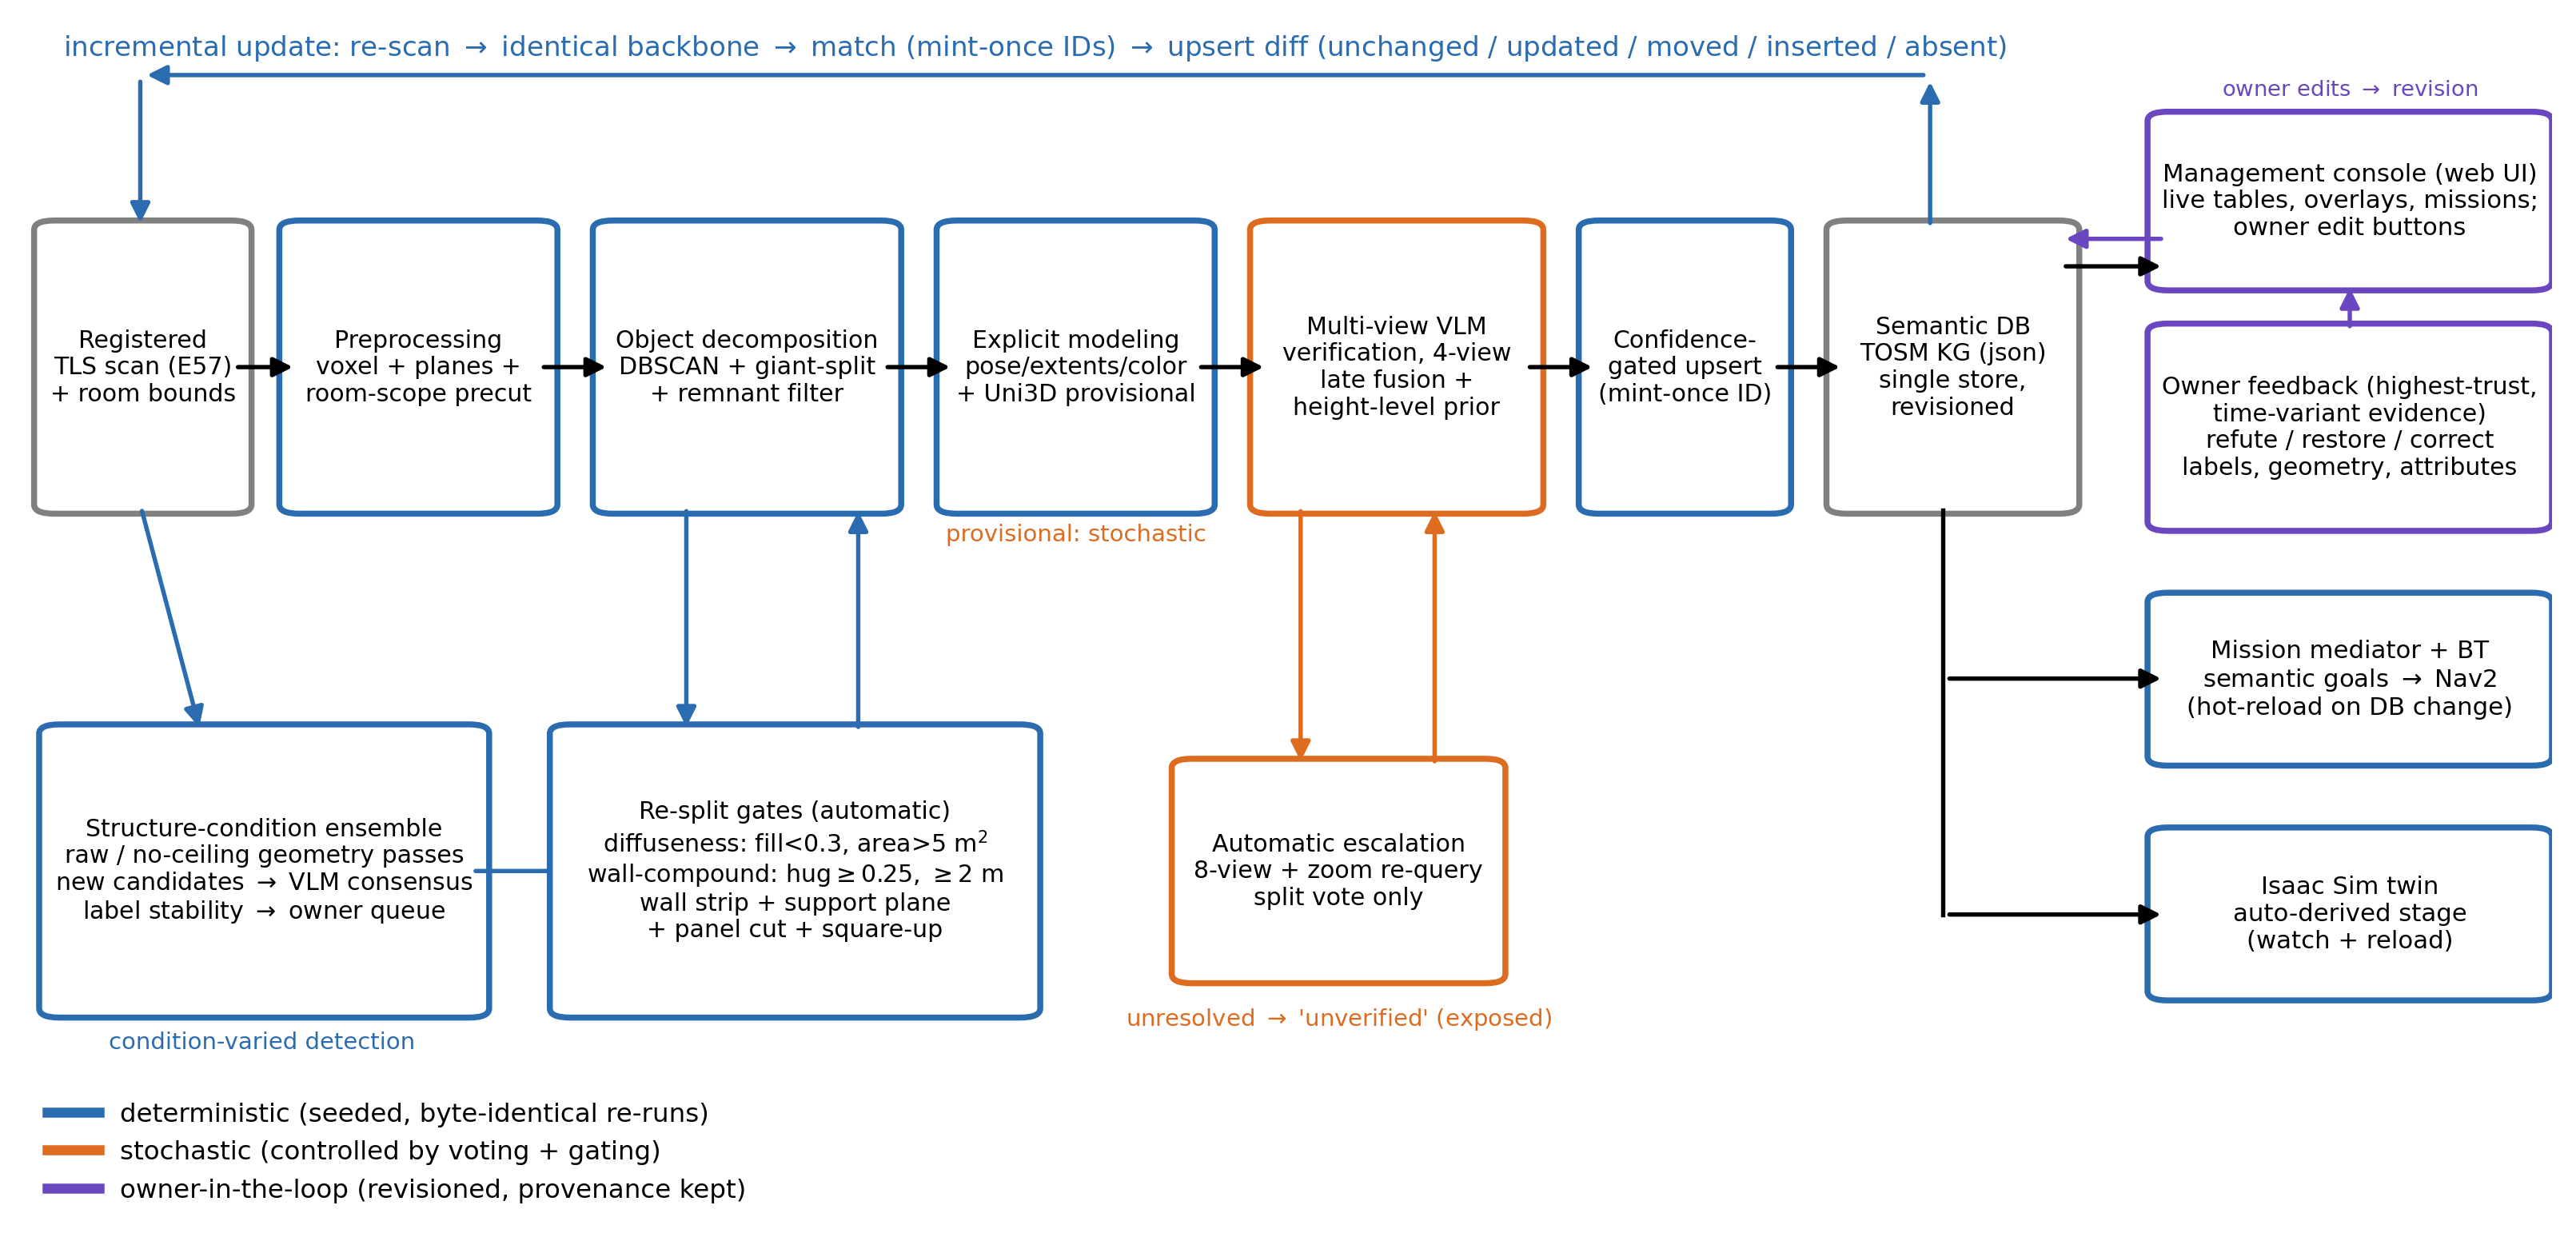
\includegraphics[width=0.95\linewidth]{fig1_architecture.png}
\caption{Framework architecture. Green stages form the deterministic
geometric backbone; orange stages are probabilistic semantic inference under
voting, escalation, and gating control. Two loops: automatic escalation
(within verification) and incremental update (across scans).}
\label{fig:architecture}
\end{figure}

\section{Methodology}
\label{sec:methodology}

This section describes the six processing stages of the framework in the
order data flows through them: TLS preprocessing (\ref{sec:preprocess}),
geometric object decomposition with structure-remnant filtering
(\ref{sec:decomposition}), explicit modeling and provisional classification
(\ref{sec:explicit}), multi-view VLM verification with automatic escalation
(\ref{sec:verification}), object identity matching (\ref{sec:matching}), and
confidence-gated graph upsert (\ref{sec:upsert}), followed by the structurally
gated query interface (\ref{sec:query}) and the object-grounded place layer
(\ref{sec:place}). Two further mechanism families---the corrective
decomposition layers with the structure-condition ensemble, and the
owner-evidence revision path---are defined in Sec.~\ref{sec:corrective},
with the failures that motivated them reported in
Secs.~\ref{sec:exp-seg} and~\ref{sec:exp-owner}; for brevity we refer
to the geometric stages through explicit modeling as \emph{Stage~A} and
to VLM verification as \emph{Stage~B}. Stages \ref{sec:preprocess}--\ref{sec:explicit} form the
\emph{deterministic geometric backbone}: every random draw is seeded, so a
re-run on the same host reproduces every retained cluster byte-identically
(Sec.~\ref{sec:exp-seg}). Stages \ref{sec:verification} onward are \emph{probabilistic
semantic inference}, controlled by voting, escalation, and confidence gating
rather than by determinism claims. The pipeline is fully automated
\emph{after registered TLS input}: the only manual steps are operating the
scanner and the vendor registration of multi-setup scans.

\subsection{TLS Preprocessing}
\label{sec:preprocess}

The input is a registered E57 point cloud from a survey-grade terrestrial
scanner (Leica BLK360). When the export contains multiple setups, the loader
applies each setup's registered pose and merges them into a single cloud; a
70M-point six-setup scan and a pre-merged single-scan export are treated
identically. The cloud is voxel-downsampled at 3\,cm---dense enough to retain
object detail while bounding the cost of all later stages. The cloud is kept
in the scanner's registered frame; no global normalization is applied.
Instead, the floor height is estimated where a stage needs it, by a robust
statistic suited to that stage's input (the densest 5\,cm height bin of the
lower half-cloud for the remnant filter; the lower quartile of per-cluster
bottom heights for the map-based filter of
Sec.~\ref{sec:corrective}).

Structural surfaces are then removed by iterative RANSAC plane
extraction~\cite{fischler1981ransac}. Each round draws 300 seeded random
point triples, keeps the candidate with the most inliers at a 5\,cm distance
threshold, and refits it once by a least-squares (SVD) fit to those inliers.
A plane is removed only if it is structural by orientation: near-horizontal
($|n_z|\ge0.85$; floors, ceilings, split ceiling levels) or near-vertical
($|n_z|\le0.2$; walls). The loop stops at the first of four conditions:
(i)~ten planes have been removed, (ii)~fewer than 2{,}000 points remain,
(iii)~the best remaining plane supports less than 4\% of the points still
present---no large plane is left---or (iv)~the best remaining plane is
slanted ($0.2<|n_z|<0.85$), i.e., object-like, so removing it would begin
carving objects. The fixed seed makes the extraction deterministic; the
pre-removal cloud is retained as a \emph{ceiling reference}
for the remnant filter of Sec.~\ref{sec:decomposition} and for incremental
re-runs. Fig.~\ref{fig:pipeline}a,b show a scan before and after
structural-plane removal.

\subsection{Geometric Object Decomposition and Structure-Remnant Filtering}
\label{sec:decomposition}

The structure-free cloud is partitioned into object candidates by
fixed-parameter DBSCAN~\cite{ester1996dbscan}
(\mbox{$\varepsilon=0.30$\,m}, 100-point minimum),
followed by a \emph{conservative giant-split}: any cluster whose horizontal
footprint exceeds 2.5\,m is re-clustered at a tighter
\mbox{$\varepsilon=0.20$\,m}, and the split is accepted only if it yields at
least two sub-clusters of 100+ points---separating merged neighbors without
shattering genuinely large equipment. We position this stage deliberately:
it is not a novel segmentation algorithm but a \emph{reproducible
decomposition designed for verification and incremental diffing}. Its value
is that identical inputs yield identical clusters with stable ordering, which
later stages exploit for result carry-over and change detection
(Sec.~\ref{sec:matching}). Fig.~\ref{fig:pipeline}c shows the resulting
instances, and Fig.~\ref{fig:pipeline}d two of the TOSM records they
eventually populate. The parameter sensitivity of this choice is
quantified in Sec.~\ref{sec:exp-seg}. Four automatic corrective layers and
one human-in-the-loop channel extend this conservative backbone; they are
defined, with their trigger conditions and parameters, in
Sec.~\ref{sec:corrective}.

\paragraph{Structure-remnant filter.}
Real buildings violate the implicit assumption that structure is planar and
objects are not. Our showroom scene has a three-level ceiling
($z=2.48/2.18/1.95$\,m): RANSAC removes each horizontal ceiling plane, but the
\emph{vertical soffit bands} at the level transitions survive removal and
surface as phantom objects (Fig.~\ref{fig:pipeline}e)---thin, wall-colored
slabs that a downstream verifier confidently misreads (e.g., as wall-mounted
keyboards or handrails, Sec.~\ref{sec:exp-verify}). We therefore filter any
cluster that passes all of the following tests, with the thresholds fixed
once and used unchanged on every scene. (i)~\emph{Soffit-scale geometry}: the
cluster's vertical extent is at most 0.6\,m and its bottom is at least
1.5\,m above the floor. (ii)~\emph{Thin vertical planar band}: the best-fit
plane (SVD) has $|n_z|\le0.25$ and an RMS off-plane thickness of at most
3\,cm. (iii)~\emph{Ceiling above}: the cluster's footprint, padded by
0.3\,m, contains at least 40 pre-removal points in the band from 2\,cm to
45\,cm above the cluster top, and (iv)~\emph{dense horizontal layer}: at
least 60\% of those points concentrate in a single $\sim$7\,cm slab around
the modal 3.5\,cm height bin---i.e., the band hangs from a real ceiling.
(v)~\emph{Topmost layer}: the region above that slab (0.1--1.5\,m higher)
holds at most 20\% as many points as the slab itself; window sills and wall
remnants fail this test because wall continues above them. The filter reduced the
showroom scene from 45 to 38 clusters and the robot hall from 88 to 81 while
leaving every retained cluster byte-identical, so previously computed
verification results remain valid. Horizontal and sloped ceiling patches are
out of the filter's scope and are discussed as a residual limitation in
Sec.~\ref{sec:discussion}.

\begin{figure}[!tp]
\centering
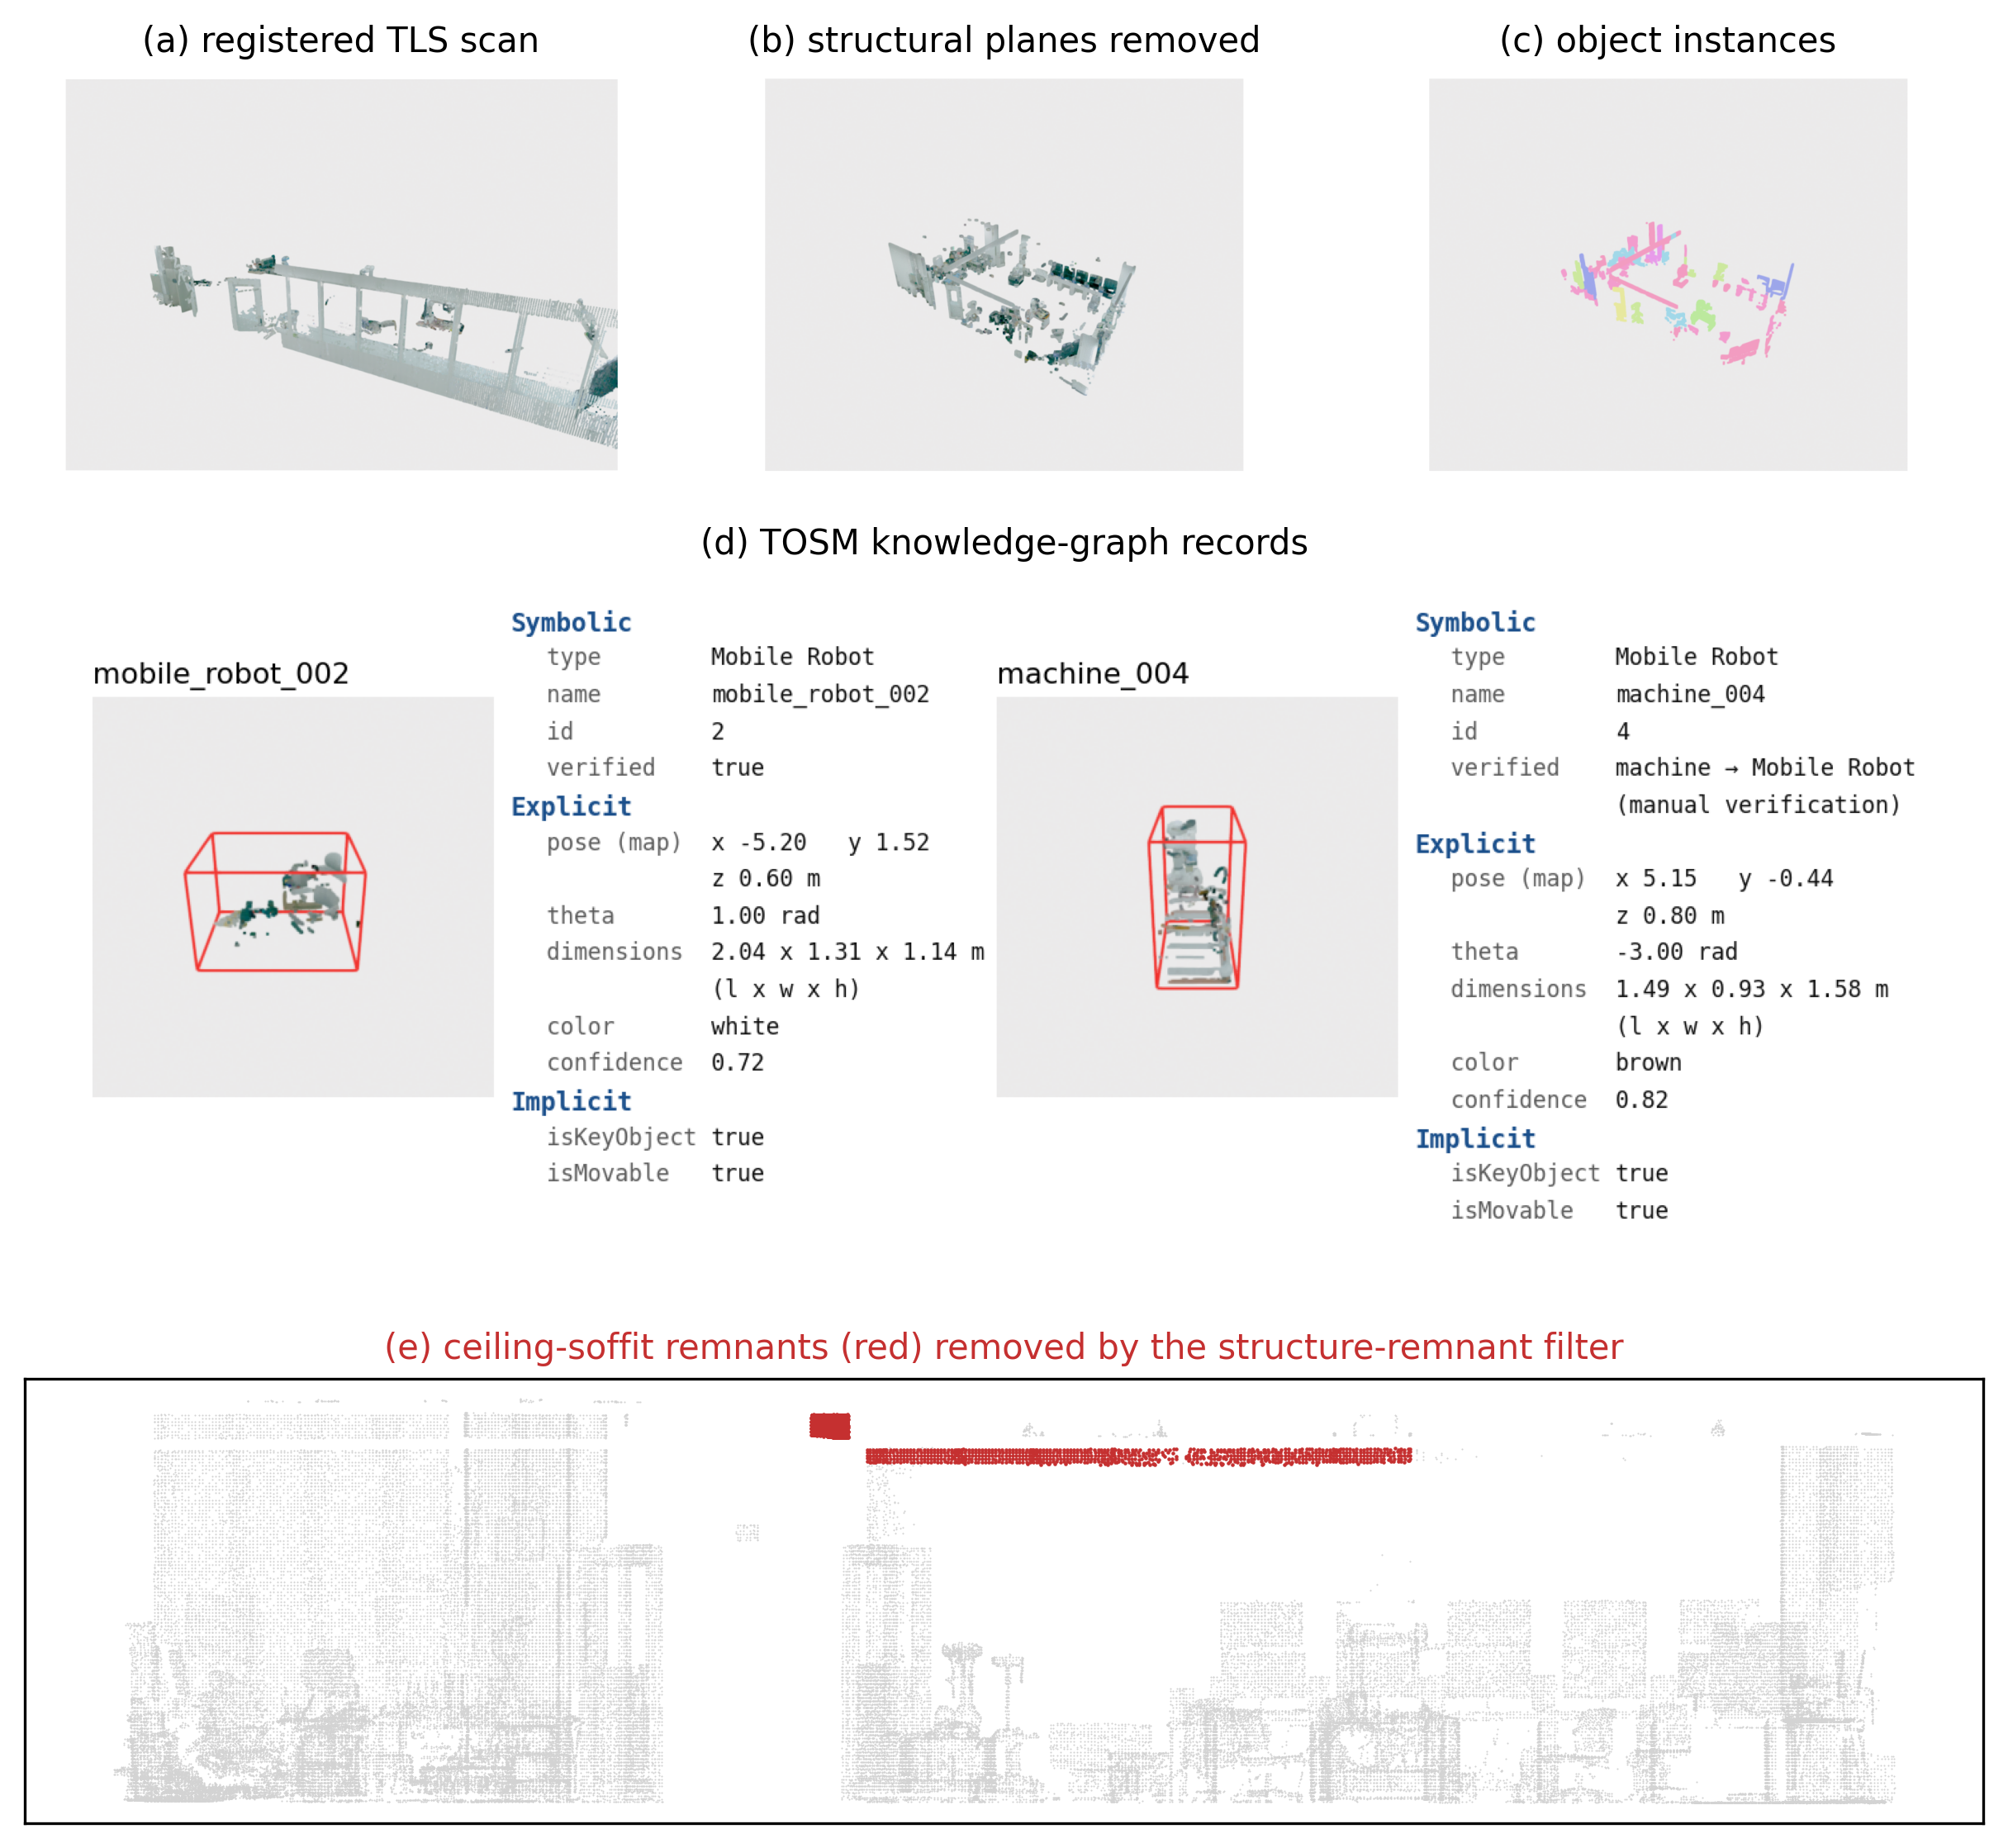
\includegraphics[width=0.92\linewidth]{fig2_pipeline.png}
\caption{Geometric backbone of TLS-SMF, illustrated on the test-room scene.
(a)~Registered multi-station TLS scan after preprocessing.
(b)~The same cloud after seeded-RANSAC removal of structural planes (floor,
walls, ceiling).
(c)~Deterministic decomposition of the residual cloud into object instances;
colors denote cluster identity, and identical inputs reproduce identical
clusters with stable ordering.
(d)~Two of the resulting TOSM knowledge-graph records with their symbolic,
explicit, and implicit attributes; \texttt{machine\_004} carries an
owner-verified type correction (\emph{machine}\,$\rightarrow$\,\emph{Mobile
Robot}).
(e)~Structure-remnant filter, shown as a front elevation of the showroom
scene: the vertical soffit bands at the three-level ceiling transitions
(red) survive horizontal-plane removal and would otherwise surface as
phantom objects; the filter removes them while leaving every retained
cluster byte-identical.}
\label{fig:pipeline}
\end{figure}

\subsection{Explicit Modeling and Provisional Classification}
\label{sec:explicit}

Each cluster is summarized by an explicit model: axis extents and centroid,
yaw from the principal component of the horizontal point distribution,
dominant color, and point count. These attributes are deterministic functions
of the cluster; the backbone's determinism claim covers geometry and these
explicit attributes only---the provisional label below is stochastic and
excluded from it. A provisional semantic label is then attached by Uni3D
open-vocabulary classification over a 30-class industrial vocabulary. The
provisional label is explicitly \emph{not trusted}: our own vocabulary
ablation shows that narrowing the vocabulary to the deployment
domain \emph{reduces} accuracy (Sec.~\ref{sec:exp-ablation}). The
provisional label serves only as VLM context and as a fallback name; every
label a robot may act on must pass the verification stage below.

\subsection{Multi-View VLM Verification with Automatic Escalation}
\label{sec:verification}

Verification renders each object from four azimuths ($0^{\circ}$,
$90^{\circ}$, $180^{\circ}$, $270^{\circ}$) and submits each view
independently to a vision--language model under a forced tool-use
schema: the model must return a type, a confidence, and a stated reason, with
the object's measured dimensions and provisional label provided as context.
Free-text answers are impossible by construction, and prompts, decoding
parameters, and model version are recorded with every result. The verifier
model itself is a swappable component, not part of the design: the concrete
model is an experimental control (Sec.~\ref{sec:setup}), and Sec.~\ref{sec:exp-ablation} repeats the
identical protocol across five commercial VLMs to characterize how the
choice affects decisiveness, accuracy, and cost.

Per-view votes are combined by confidence-weighted late fusion. Let view $v$
return label $\ell_v$ (lowercased; no synonym mapping is applied at fusion
time) with confidence $c_v\in[0,1]$. Each candidate label accumulates the
\emph{sum} of the confidences of the views that voted for it,
$s(\ell)=\sum_{v:\,\ell_v=\ell}c_v$; the fused type is
$\hat{\ell}=\arg\max_{\ell}s(\ell)$, and the \emph{vote share} is its
normalized confidence mass, $\sigma=s(\hat{\ell})/\sum_{\ell}s(\ell)$.
A confidence-weighted sum, rather than a view count, lets one hesitant
dissenter matter less than a confident one. Three outcomes follow
(Fig.~\ref{fig:escalation}). If the votes are
unanimous, the object is \texttt{verified}; unanimity is empirically a strong
signal (94.4--100\% precision on the two scenes' confirmed ground truth,
Sec.~\ref{sec:exp-verify}),
although Sec.~\ref{sec:exp-verify} also documents its failure modes. If the vote splits, the
object \emph{escalates automatically}: eight additional images---four diagonal
azimuths and four zoomed close-ups---are classified, and the fusion is
recomputed over all twelve votes pooled (the base four included). If the
post-escalation share reaches $\sigma\ge0.6$
the object becomes \texttt{verified\_escalated}; otherwise it remains
\texttt{unverified}. The 0.6 threshold was fixed a~priori, before any
evaluation, as the smallest round value that demands a clear supermajority
of the confidence mass: at 0.5 a twelve-view vote split between two labels
of equal confidence could verify on a tie-break, whereas 0.6 requires the
winning label to dominate all alternatives combined by a margin. The
threshold gates \emph{status only}---the fused label is recorded either
way---so its effect is a precision--recall trade on the verified tier;
Sec.~\ref{sec:exp-verify} re-scores the stored votes across a threshold
sweep to quantify that trade. Crucially, unresolved objects are not hidden, discarded,
or resolved by a human: they stay in the graph with their failed candidate
label attached, and the query interface (Sec.~\ref{sec:query}) is responsible
for making their status impossible to ignore. Implicit robot-facing
attributes (movability, openability, key-object status) are inferred once at
fusion time from the winning view set.

Escalation bounds cost: only split votes pay for the wider view set
(trigger rates 51--58\%, Sec.~\ref{sec:exp-verify}), and per-call cost is $\sim$\$0.009, so a
scene verifies for a few dollars (Sec.~\ref{sec:discussion}).

\begin{figure}[t]
\centering
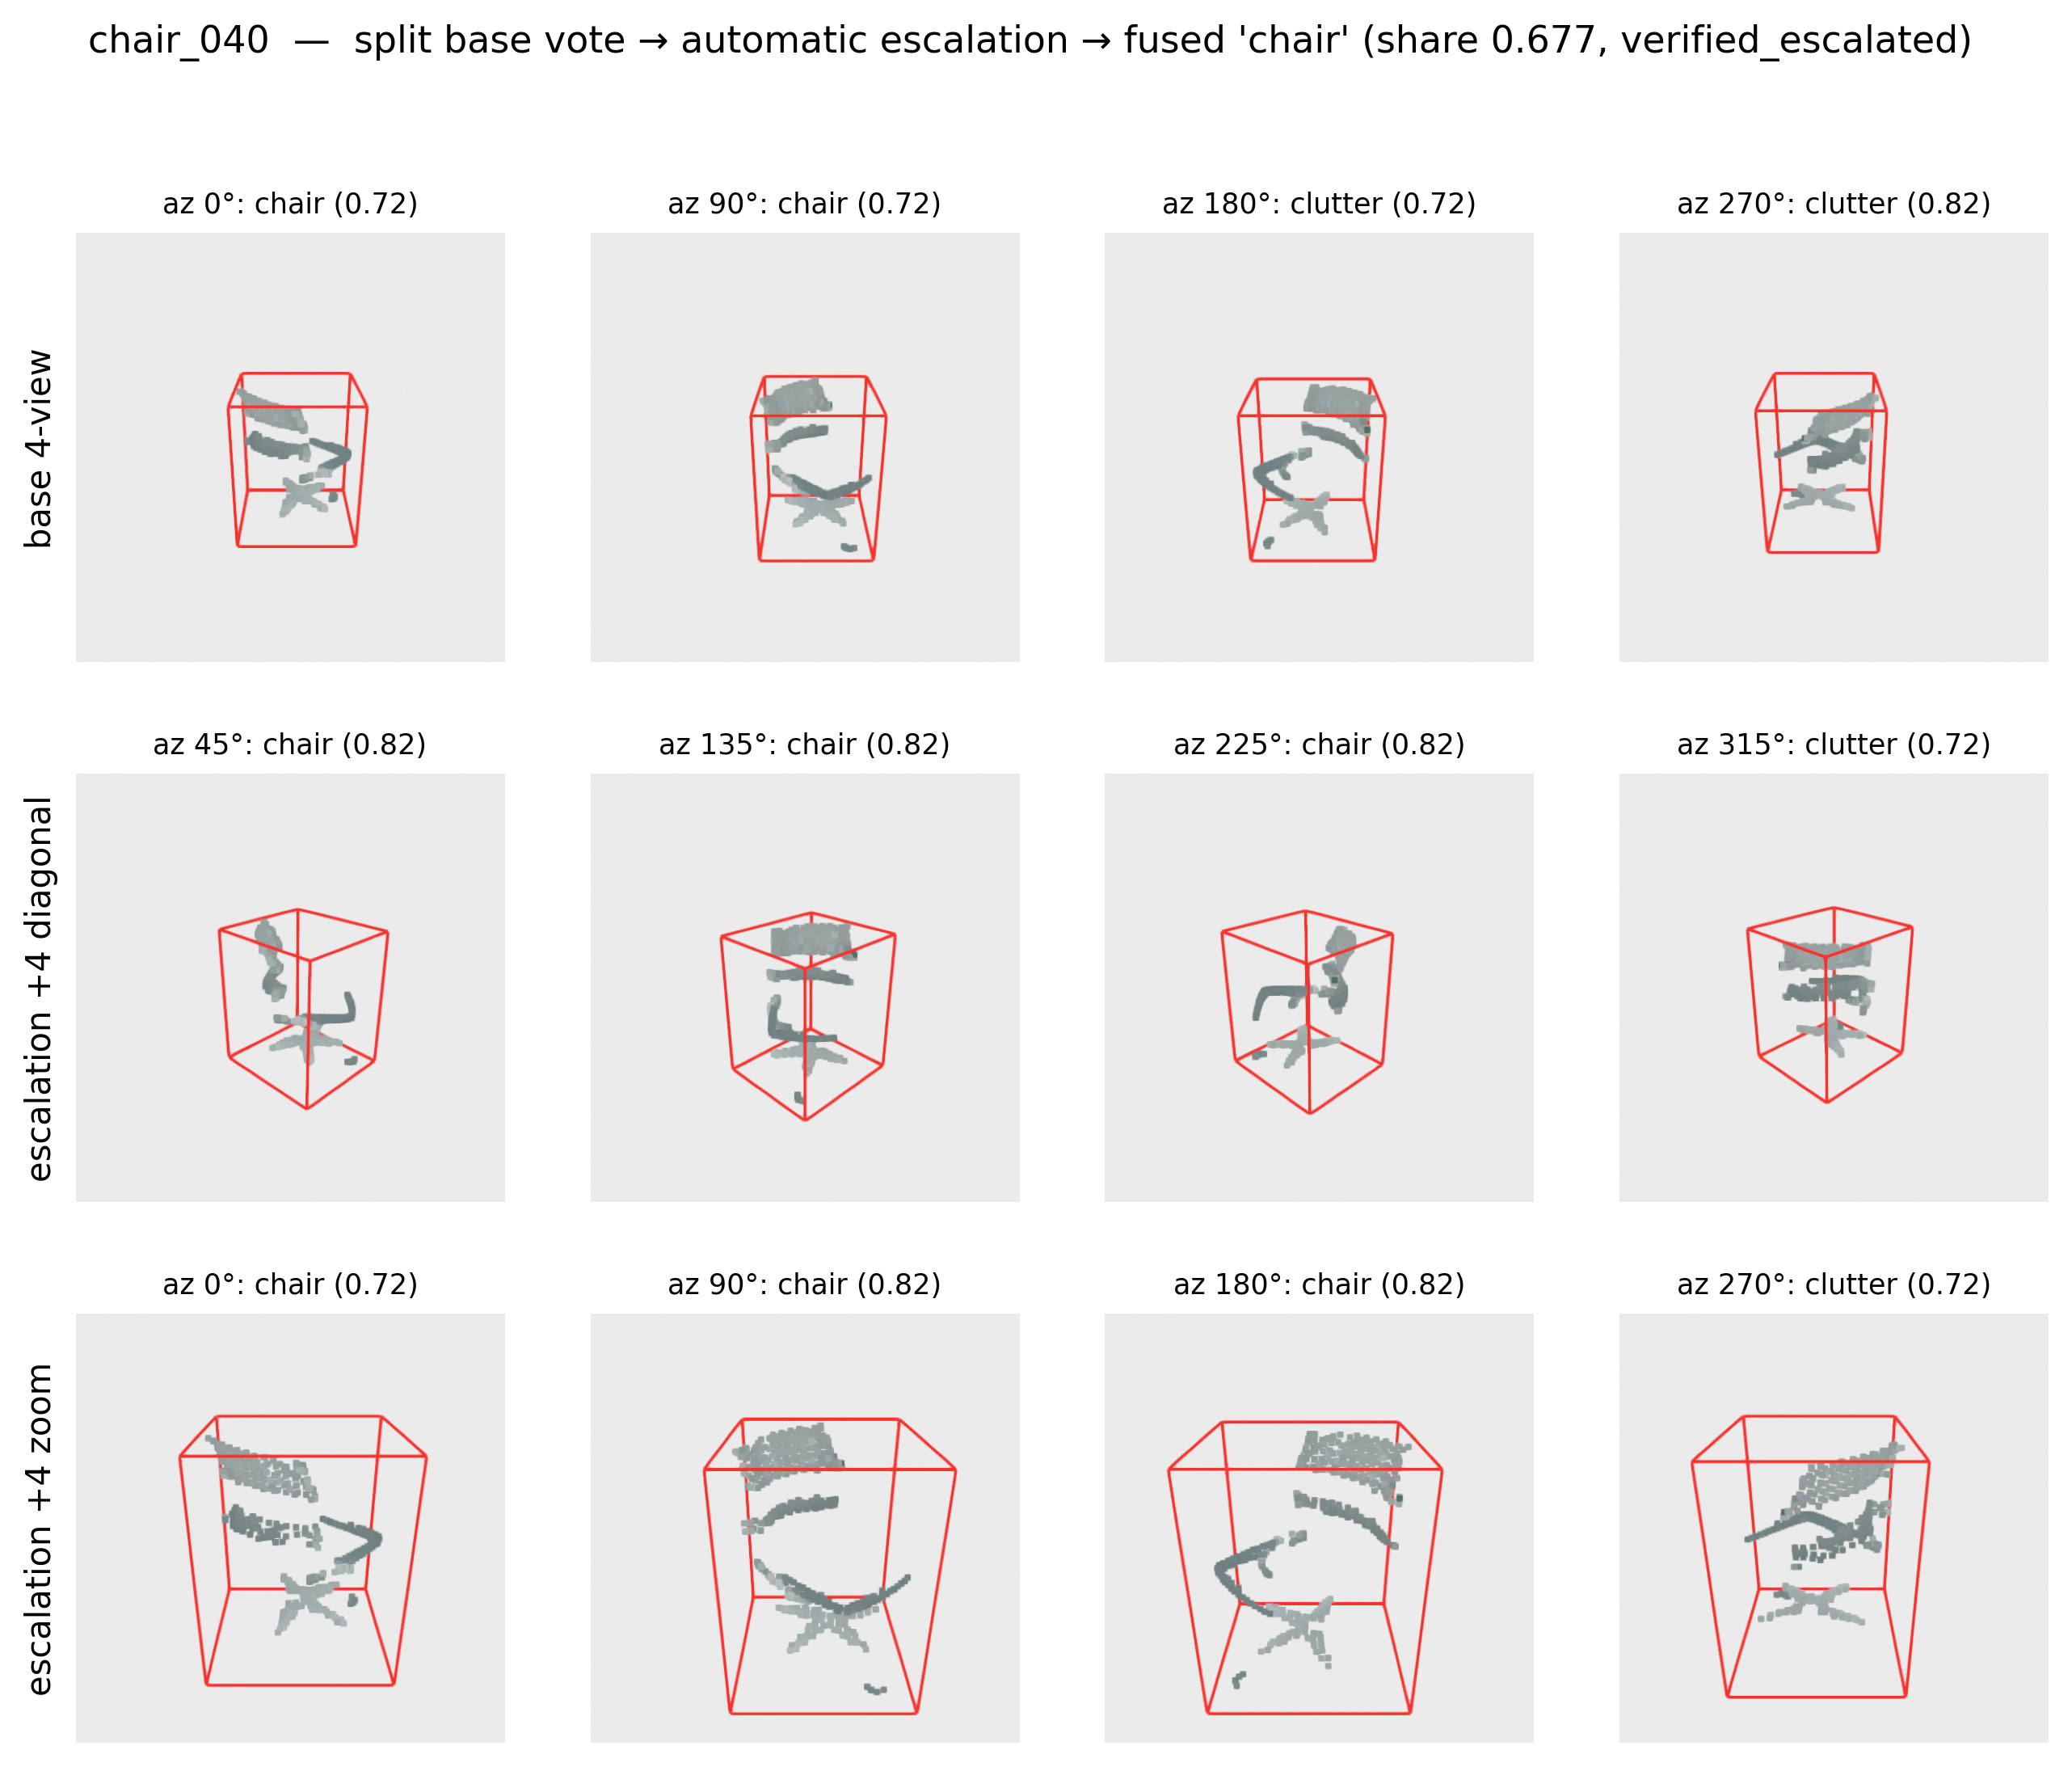
\includegraphics[width=0.95\linewidth]{fig3_multiview_escalation.png}
\caption{Multi-view verification and automatic escalation, with per-view
votes, fused share, and the three terminal statuses.}
\label{fig:escalation}
\end{figure}

\subsection{Object Identity Matching}
\label{sec:matching}

The update problem is an \emph{identity} problem before it is a geometry
problem: a robot that plans against node IDs needs yesterday's chair to be
today's chair. Our policy is \textbf{mint-once}: a node ID is minted when an
object first enters the graph---derived from a fingerprint of its birth-time
anchor (map, position, extent)---and never changes afterwards. The
fingerprint is a candidate-retrieval key, not the identity itself; after
minting, matching alone carries identity forward.

Matching between a new scan's records and existing nodes runs in two passes:

\begin{enumerate}
\item \textbf{Spatial pass.} A record matches a node if their 3-D centroids
agree within 0.5\,m and each of the three extents (length, width, height)
agrees within a per-axis tolerance of $\max(0.3\cdot
\max(d_{\mathrm{old}},d_{\mathrm{new}}),\,0.15\,\mathrm{m})$---a 30\%
relative band with a 15\,cm absolute floor so that small objects are not
over-constrained. No type constraint applies in this pass; a changed label
on a geometrically stable object is recorded as an update, not a new
object. Matches update pose and extents in place (\texttt{unchanged} /
\texttt{updated}).
\item \textbf{Move pass.} Remaining records match remaining nodes of the
\emph{same type} with dimensions consistent under the same per-axis
tolerance, within a 6\,m horizontal search radius,
producing \texttt{moved} nodes with preserved IDs. Generic types
(\texttt{clutter}, \texttt{unknown}) are excluded from this pass: a generic
label carries too little identity for displacement claims, and our real
two-epoch data showed that admitting them fabricates 2--5\,m
``moves'' between unrelated piles (Sec.~\ref{sec:exp-update}).
\end{enumerate}

\emph{Conflict resolution.} When several nodes satisfy the predicate for one
record, the record claims the node with the smallest horizontal centroid
distance; when several records compete for one node, the first claim wins
and the node is removed from the candidate pool, so later records fall
through to the move pass and then to insertion. Assignment is therefore
greedy in record order rather than a global optimum---a deliberate
simplicity choice: records arrive in the backbone's deterministic cluster
order, so the assignment itself is reproducible, and at the object densities
of our scenes ($\le$0.6 objects/m$^2$) multi-candidate conflicts are rare
(Sec.~\ref{sec:exp-update} reports the observed conflict counts).
The thresholds encode physical priors rather than tuned values: 0.5\,m is
below the smallest inter-object spacing we expect a scan-to-scan pose drift
to produce for a stationary object (and is far above the $\le$5\,cm
registration residual, Sec.~\ref{sec:setup}); the 30\%/0.15\,m extent band
absorbs partial-view truncation between scans without admitting
differently-sized objects; and 6\,m bounds a within-room relocation. They
were fixed on the development epochs (T1/T2) and used unchanged afterwards.

Records that match nothing are minted as new nodes (\texttt{inserted});
nodes that no record claims are marked \texttt{absent} but retained with
their full history, so an object that returns later resumes its original
identity. Sec.~\ref{sec:exp-update} evaluates matching accuracy, identity-switch rate, and
false-new/false-absent rates, including the occlusion level at which
matching breaks (40\% crop).

\subsection{Confidence-Gated Graph Upsert}
\label{sec:upsert}

Each scan epoch applies its matched record set to the knowledge graph as a
node-level upsert---no rebuild. Every node carries its verification status,
provenance (per-view votes, fused share, escalation flag, model version), a
per-revision history of every change, and \texttt{firstSeen}/\texttt{lastSeen}
timestamps. Edges (spatial relations---\texttt{isNextTo}, \texttt{isOn},
\texttt{isAboveOf}---recomputed from explicit models) are scoped to the map
and revision, and organized by the place layer: \texttt{isNextTo} is kept
only between objects of the same place (proximity across a place boundary
is expressed at the place level as \texttt{isAdjacentTo}), vertical
relations must pass a rotated-footprint overlap test (a separating-axis
check that discards the long-range stacked relations oversized merged
clusters otherwise produce), and each place designates a key object
(the VLM's implicit \texttt{isKeyObject} among verified members, falling
back to the most confident specific-type verified member; objects refuted
by owner ground-truth feedback are excluded from designation while
remaining in the graph as annotated errors). On the T3
epoch this scoping removes 24 of 49 raw proximity edges---long
cross-place spokes centered on the largest cluster---leaving 25
intra-place edges over 11 place adjacencies; Fig.~\ref{fig:relmap} shows
the resulting map. The result is exported both as a canonical
JSON graph and as mapId-scoped Neo4j Cypher, so multiple sites and epochs
coexist in one database. Because unchanged objects reproduce byte-identical
clusters (Sec.~\ref{sec:decomposition}), their verification results are
carried over by content hash and an identical-input repeat scan costs
\emph{zero} VLM calls;
a changed scan of the same acquisition quality pays only for changed
clusters (3.1\% of full cost in our controlled combined-edit measurement,
Sec.~\ref{sec:exp-update}). The carry-over is conditional on reproducible
acquisition: when scan quality itself changes between epochs, as in our
real T2$\rightarrow$T3 transition, no cluster hashes match and the epoch
pays full verification cost (Sec.~\ref{sec:exp-update}).
Fig.~\ref{fig:upsert} summarizes
the mint-once identity flow and the node outcomes of a re-scan.

\begin{figure}[t]
\centering
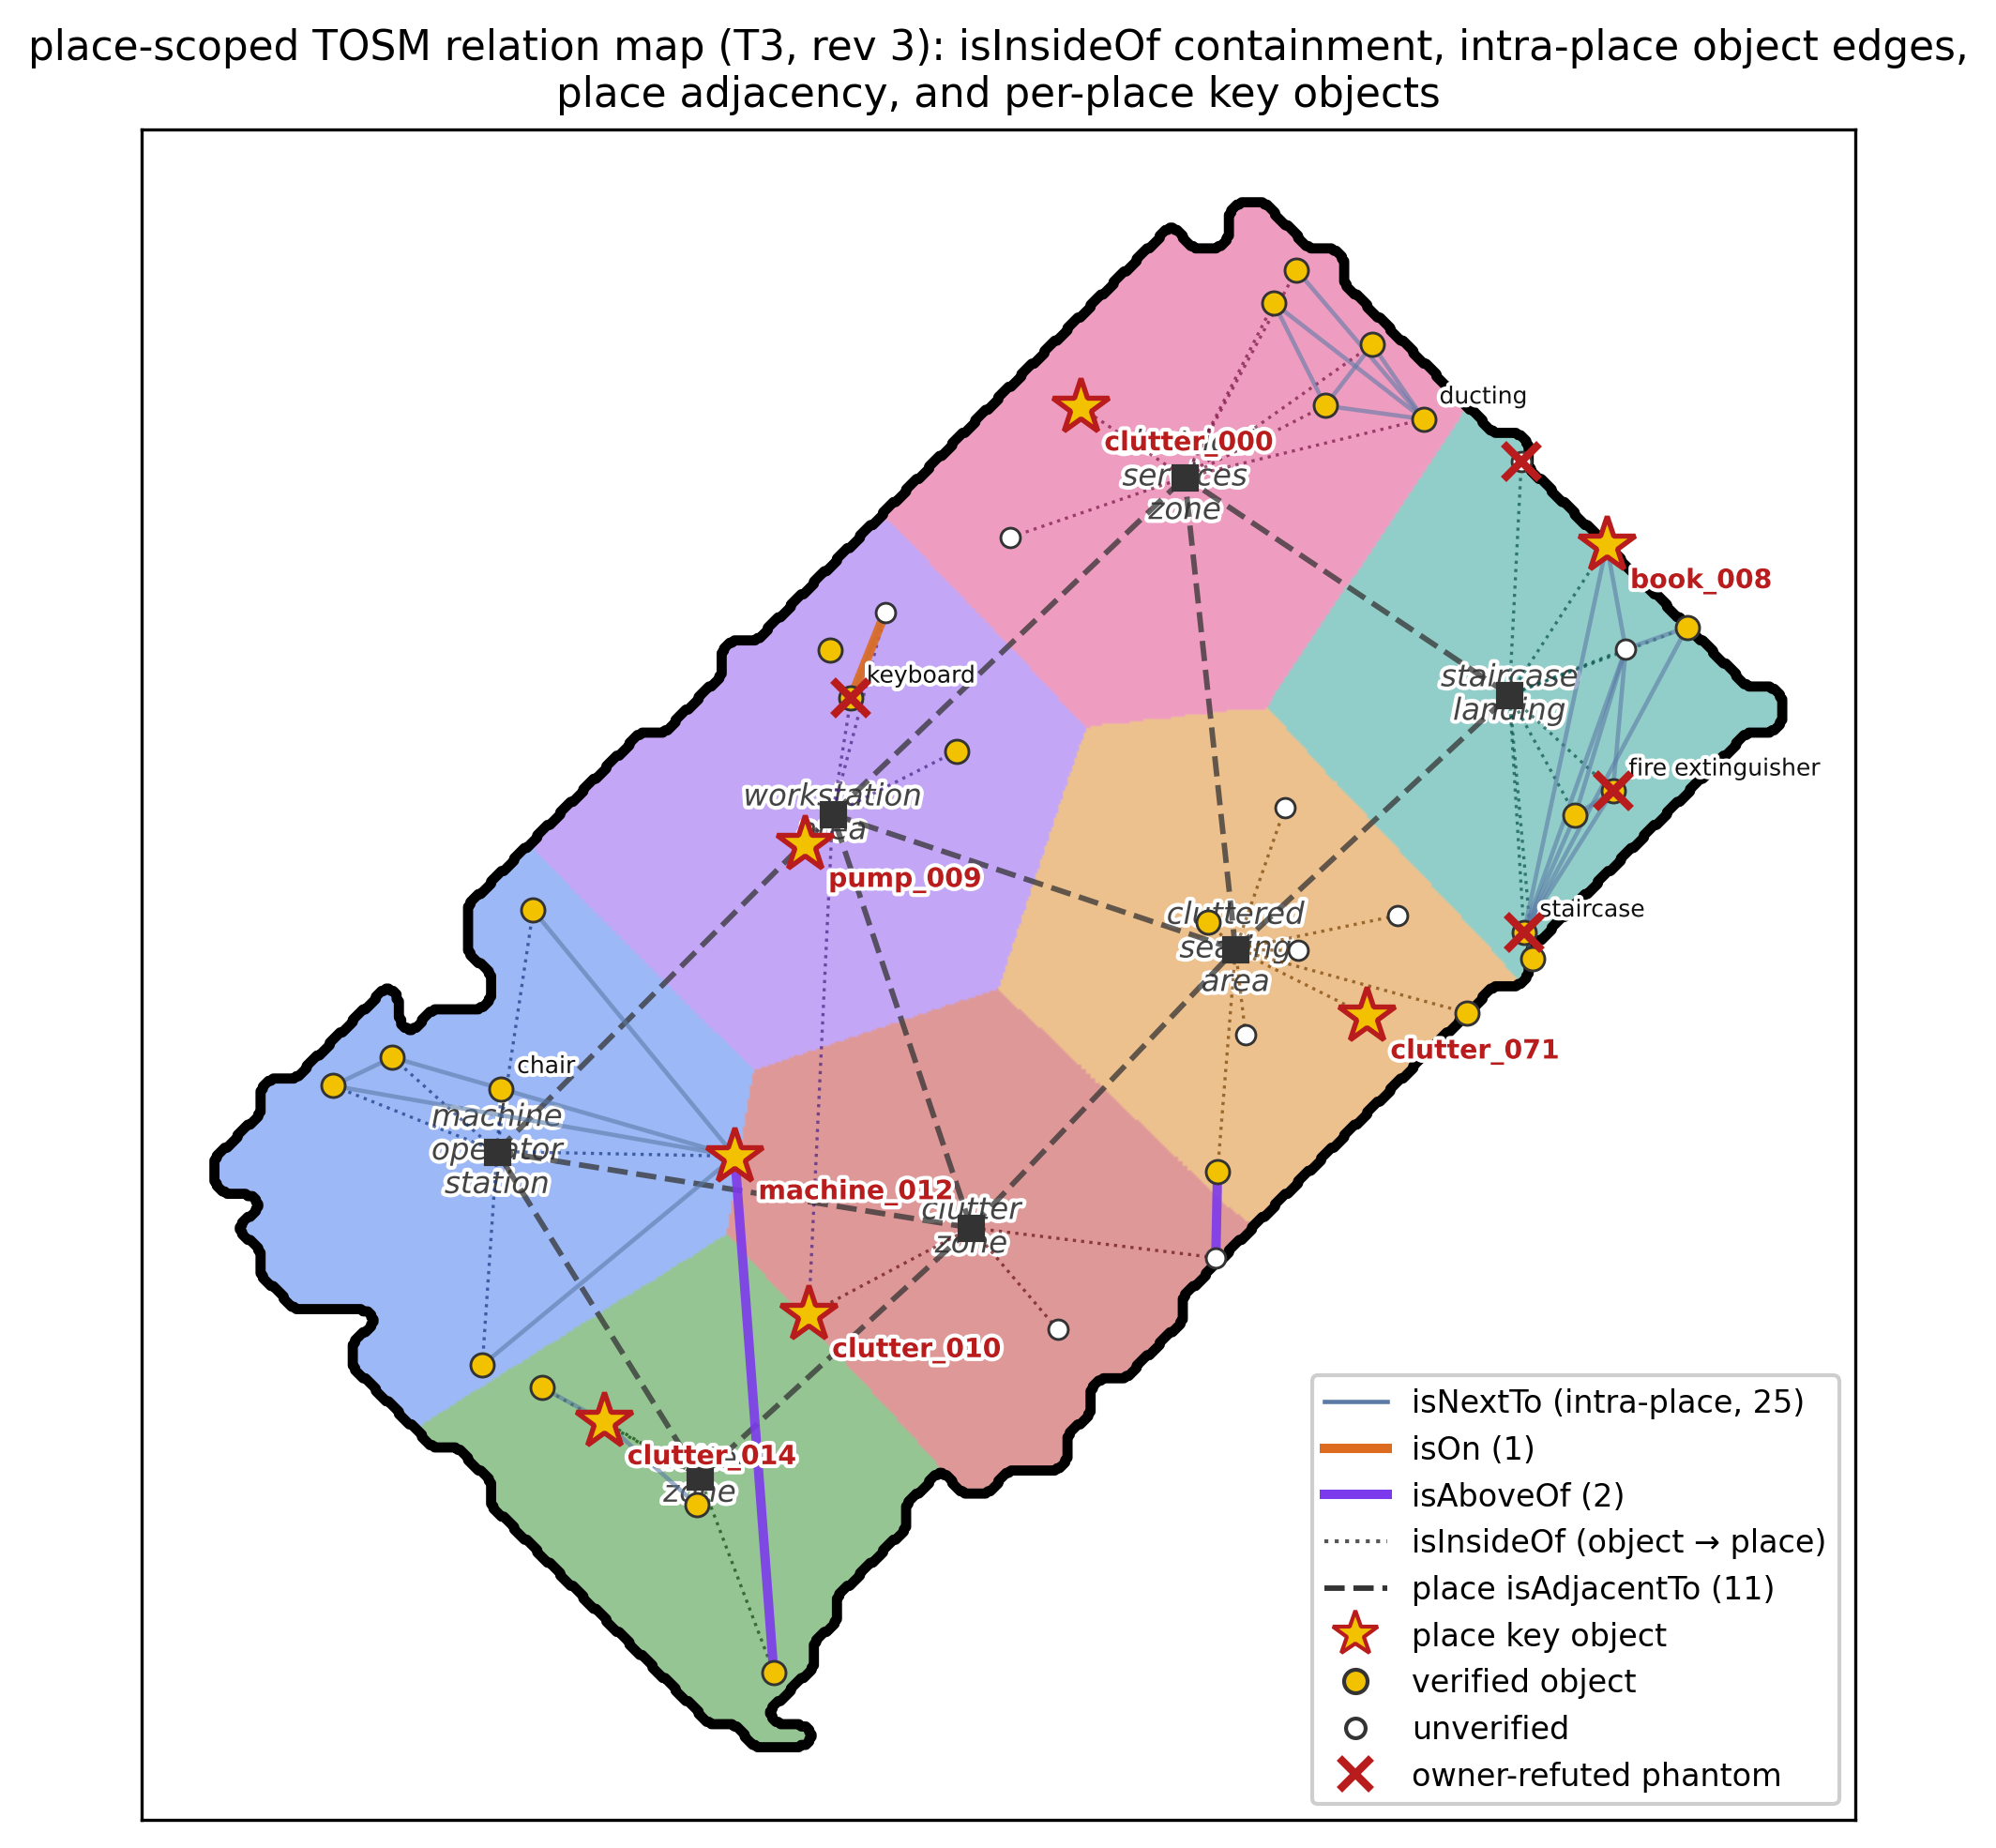
\includegraphics[width=0.85\linewidth]{fig12_relations_map.png}
\caption{Place-scoped TOSM relation map (T3) over the place layer of
Fig.~\ref{fig:placemap} (pastel): dotted object$\rightarrow$place
\texttt{isInsideOf} containment, intra-place \texttt{isNextTo} edges,
vertical \texttt{isOn}/\texttt{isAboveOf} relations, dashed place
\texttt{isAdjacentTo} edges between region centroids, and per-place key
objects (named stars). The map reflects the graph's current revision,
including owner feedback (Sec.~\ref{sec:exp-owner}).}
\label{fig:relmap}
\end{figure}

\begin{figure}[t]
\centering
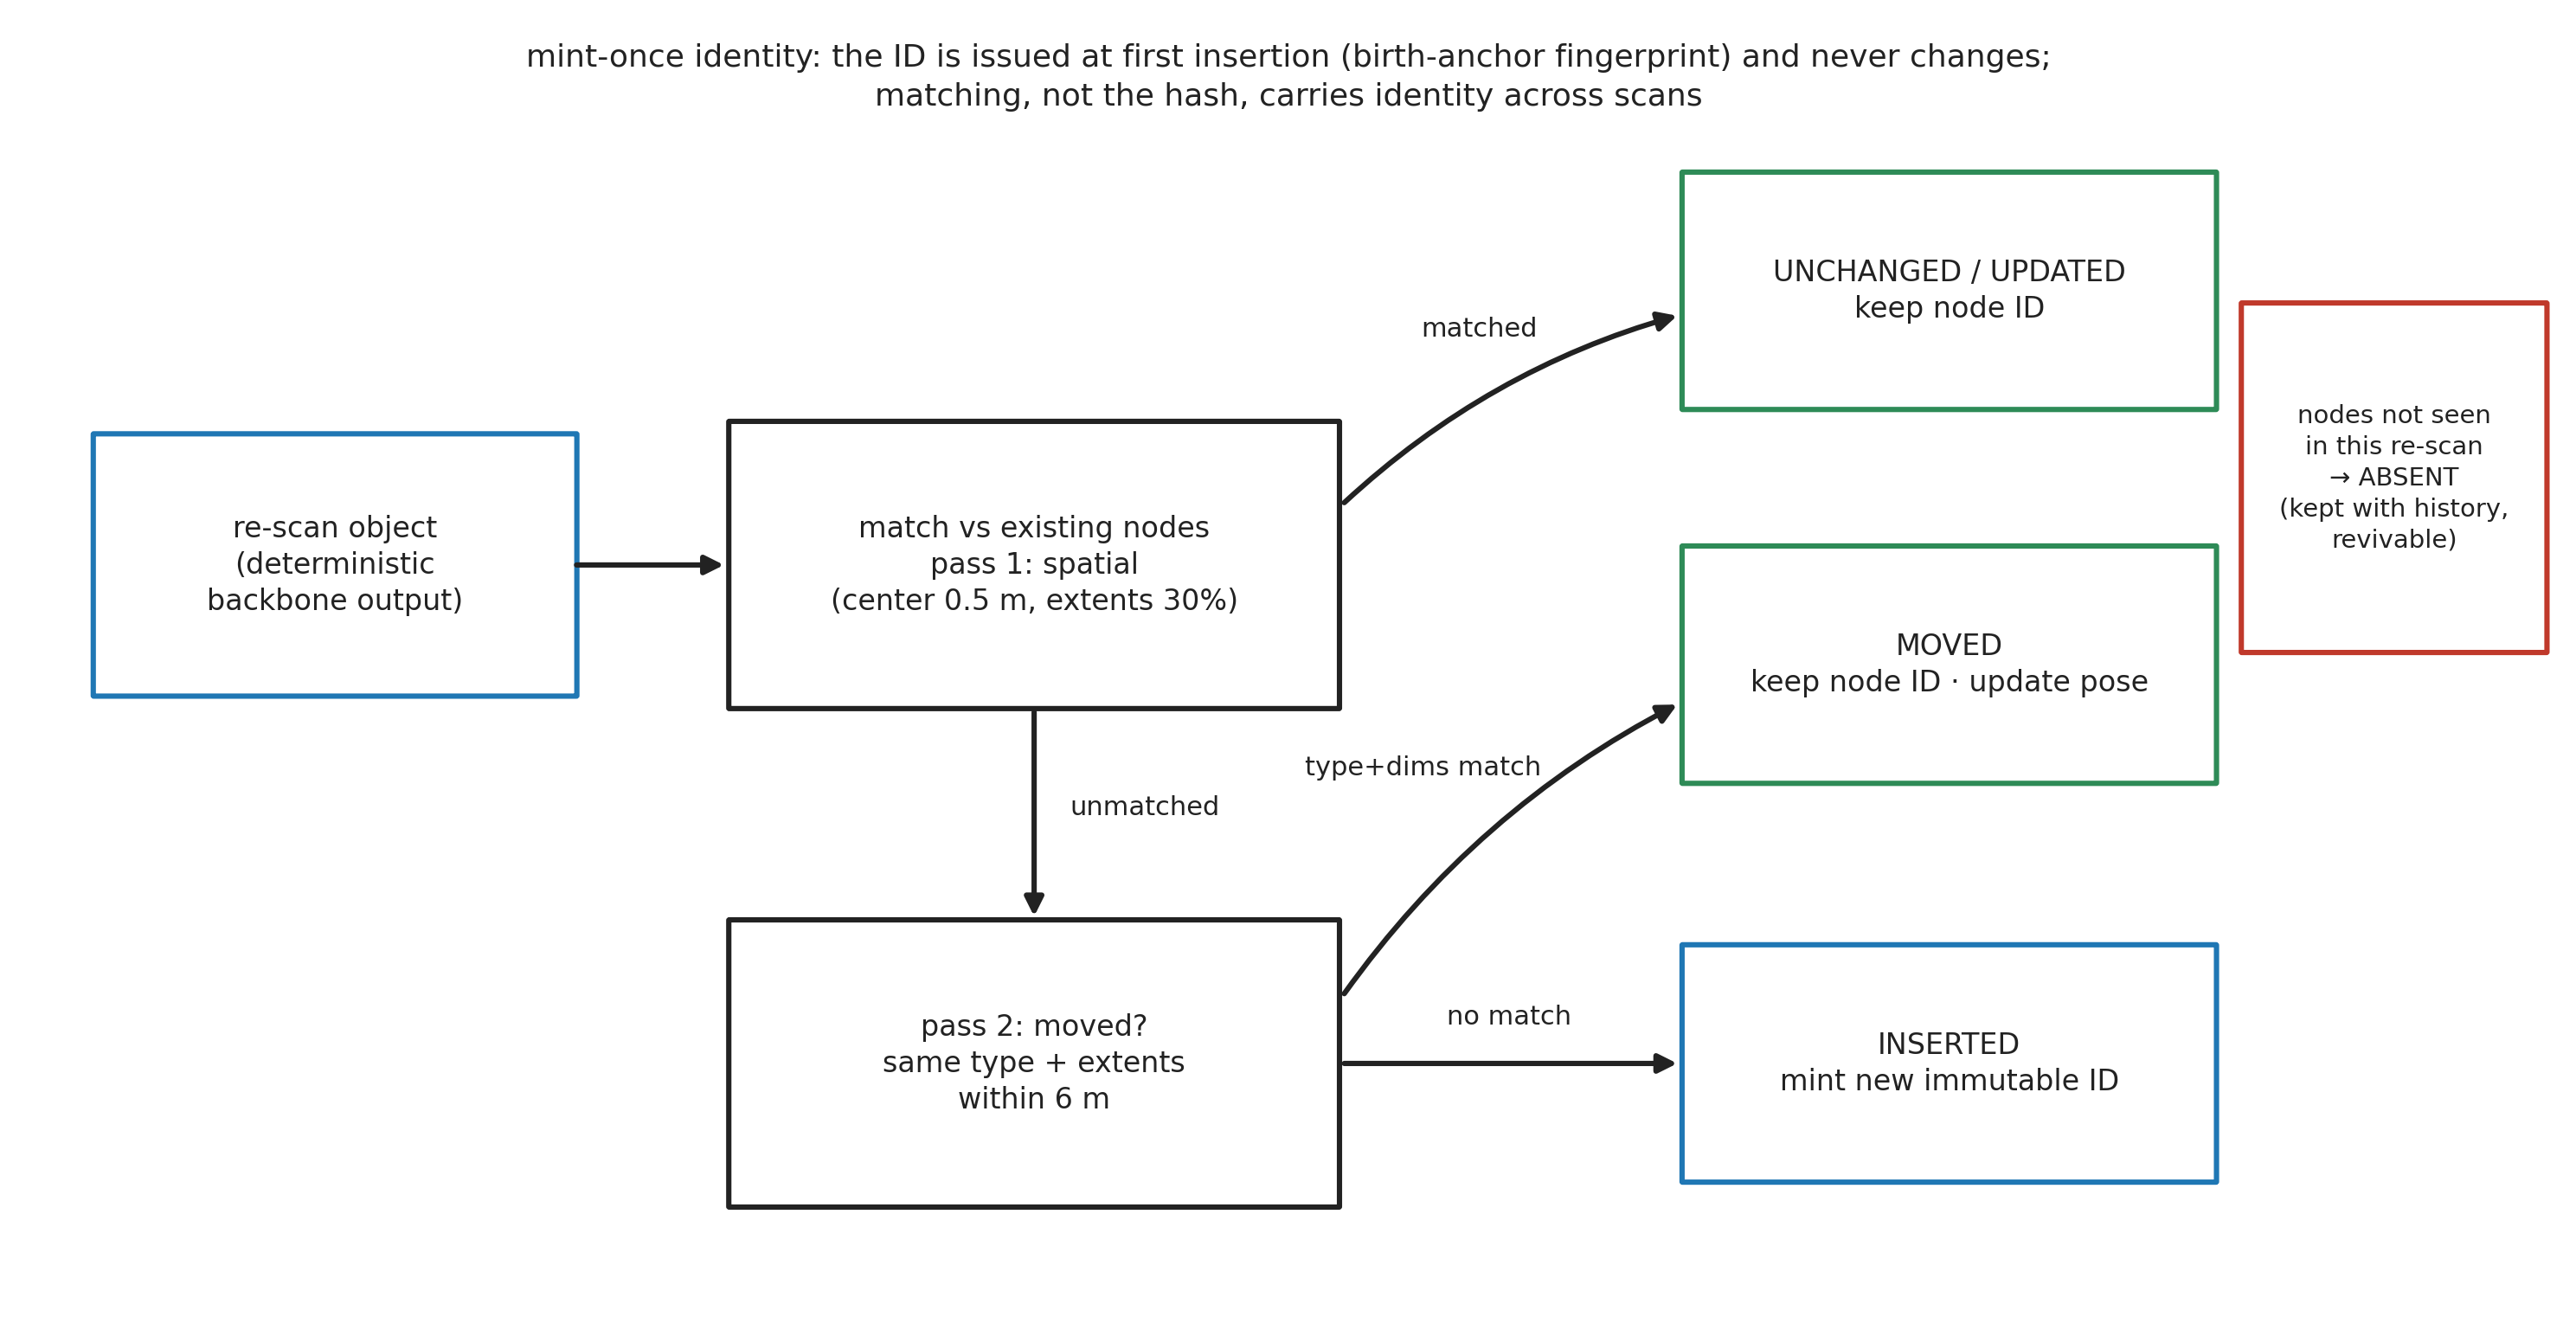
\includegraphics[width=0.9\linewidth]{fig5_identity_upsert.png}
\caption{Identity matching and confidence-gated upsert: mint-once IDs,
two-pass matching, and the five node outcomes across a re-scan.}
\label{fig:upsert}
\end{figure}

\paragraph{Formal summary.}
Consolidating the above: an object record is the tuple
$r=(a, p, d, \ell, c, \tau, \pi)$ with birth anchor $a$ (map ID plus
position and extent quantized at 0.25\,m, hashed once at first insertion),
pose $p\in SE(2)\times\mathbb{R}$, extents $d=(l,w,h)$, fused label $\ell$,
confidence $c$, verification tier $\tau$, and provenance $\pi$ (per-view
votes, share, escalation flag, model version). The tier set is
\[\begin{aligned}\mathcal{T}=\{&\texttt{verified},\ \texttt{verified\_escalated},\ \texttt{verified\_majority},\\
&\texttt{verified\_recovery},\ \texttt{verified\_owner},\ \texttt{unverified},\ \texttt{refuted}\},\end{aligned}\]
ordered by evidence
source: unanimity, escalated supermajority, agreement-gated recovery, and
owner declaration (confidence 1.0); the query gate
(Sec.~\ref{sec:query}) exposes only the verified tiers as typed objects.
The match function is
$m(n,r)=\mathbb{1}[\lVert p_n-p_r\rVert_{3\mathrm{D}}\le0.5]\cdot
\prod_{k\in\{l,w,h\}}\mathbb{1}[\,|d_{n,k}-d_{r,k}|\le
\max(0.3\max(d_{n,k},d_{r,k}),0.15)]$, with the move-pass variant
substituting a 6\,m horizontal bound and an exact-type, non-generic
constraint. The upsert decision for each record--node pair follows the
deterministic cascade \emph{match} $\rightarrow$ \emph{move} $\rightarrow$
\emph{insert}, with unclaimed nodes marked \emph{absent}; every transition
appends to the node's history, and no node is ever deleted. All numeric
constants above and in
Secs.~\ref{sec:preprocess}--\ref{sec:upsert} were fixed on the development
epochs (T1/T2) and applied unchanged to T3 and the cross-floor scene.

\subsection{Corrective Decomposition Layers and Owner Feedback}
\label{sec:corrective}

The backbone of Sec.~\ref{sec:decomposition} is deliberately conservative,
and its characteristic failures---diffuse residual webs, wall-flush
compounds amputated by structure removal, structure noise that survives
plane removal, and real objects absorbed into \texttt{clutter}---are
corrected by five layers defined here. The first four are automatic and
run inside the frozen pipeline on every epoch; the fifth is the
human-in-the-loop channel. Each was \emph{developed} in response to
failures observed on the development epochs
(Sec.~\ref{sec:exp-owner} preserves that discovery narrative and its
evaluation); their definitions, triggers, and parameters were frozen
before the cafeteria evaluation and require no per-scene parameter
adjustment at execution; held-out transfer is evaluated only where
explicitly reported in Sec.~\ref{sec:exp-endtoend}.

\begin{enumerate}
\item \textbf{Diffuseness-gated re-split.} Trigger: a cluster whose 2-D
occupancy fill (10\,cm grid) is below 0.30 while its footprint exceeds
5\,m$^2$---real objects in our scenes fill 0.5--0.85. The cluster is
re-decomposed by occupancy-core erosion: grid cells with $\ge$8 points and
$\ge$3 occupied 8-neighbors seed connected components; components with
$\ge$250 points survive. Compounds are further split at the support plane
(the $z$-histogram peak 0.5--0.95\,m above floor), with grounded cells
spanning $>$1.3\,m vertically treated as legs/poles, and under-slab
fragments re-attached at $\ge$60\% footprint overlap. An evidence gate
($\ge$250 points, $\ge$5\,m$^2$ or 12\,m$^2$ for desk banks,
$\ge$0.15\,m height) keeps only physically plausible sub-objects.
\item \textbf{Wall-compound gate.} Trigger: $\ge$25\% of a cluster's
points within 0.12\,m of the exploration-grid wall line over a span of
$\ge$2\,m, with $\ge$250 points protruding off-wall, and the cluster not
diffuse. The wall band is stripped, the support plane is detected as
above, and the panel band is cut at density valleys along the wall,
yielding unit-level decomposition of wall-mounted equipment. A final
\emph{panel square-up} pass then re-assigns every compound point that
falls inside a panel unit's bounding box, padded by 6\,cm horizontally
and 5\,cm vertically, back to that unit---drawing from the extracted
support-post pieces and from points left unassigned by the cuts---so that
post extraction and layer clustering do not leave bite marks or holes in
the panel rectangles; it is instance-segmentation finishing with no
semantic input.
\item \textbf{Structure-condition ensemble.} Trigger: every epoch.
The geometric pass is repeated under three structure-removal conditions
(none / ceiling-only / full); clusters found under an alternative
condition but absent from the production set become new candidates, and
only those are sent to verification. Cross-condition label agreement is
stored per object as a \texttt{labelStability} attribute
(stable/unstable) that prioritizes owner review; cross-condition
\emph{voting} is deliberately not used to fuse labels, because verifier
biases proved correlated across conditions
(Sec.~\ref{sec:exp-seg}).
\item \textbf{Hybrid grid-map structure filter.} Trigger: every epoch,
after clustering. Each cluster is registered against the exploration
occupancy grid (an independent, drift-free wall prior) and flagged by the
first matching rule of a fixed cascade: outside-room ($>$50\% of points
beyond the filled room polygon), ceiling fixture (bottom $>$2.0\,m above
floor), wall remnant (wall-hug fraction---the fraction of cluster points
within 0.15\,m of the nearest grid wall line---$>$0.6 with PCA minor
extent $<$0.22\,m and a horizontal minor axis), or full-height wall band
($z$-span $>$2.5\,m, per-metre-segment median thickness $<$0.3\,m,
along-wall length $>$2\,m---the length condition spares wall-mounted
panels). Flagged clusters are removed upstream of verification.
\item \textbf{Owner feedback and gated recovery.} The console exposes
four operations, each applied as a normal KG revision with history:
\emph{declare} (sets \texttt{verified\_owner} at confidence 1.0),
\emph{refute} (sets \texttt{refuted}, presence \texttt{absent}, and
exclusion from key-object designation), \emph{correct} (label or
attribute in place, the VLM verdict retained in provenance), and
\emph{re-verify}. Recovery re-verification re-asks the verifier with
\texttt{clutter} treated as \emph{unidentified}, in two independent
passes (open vocabulary; site vocabulary plus Uni3D candidates); a
recovered label is adopted---as \texttt{verified\_recovery}---only when
the two passes agree under canonical synonym matching, or a pass agrees
with the cluster's own base label, and the label is not \texttt{clutter};
a focused tie-break pass re-asks with exactly the two disputed labels and
is accepted only when its answer is one of them at confidence $\ge$0.6.
\end{enumerate}

\subsection{Query Interface with Structural Gating}
\label{sec:query}

The graph is queried through an LLM that receives a serialized view of the
relevant nodes. The naive design---instructing the model not to assert
unverified labels---fails in practice: in our benchmark the instructed model
still asserted trap labels in 3 of 4 cases (Sec.~\ref{sec:exp-ablation}). We therefore
\emph{gate by construction, not exhortation}: in the query-time view, every
unverified node's type is demoted to \texttt{unknown}, and the failed
candidate label is moved to a separate \texttt{failedCandidateType} field
whose semantics (``a classifier guess that did not survive verification'') are
stated in the schema, not in behavioral instructions. Fig.~\ref{fig:cards}
contrasts the two record states as the query interface sees them. With the
gate in the data rather than the prompt, the model cannot assert an
unverified label without visibly contradicting its input: the four
unverified-label traps are blocked in the gating-style ablation (4/4,
Sec.~\ref{sec:exp-ablation}), while in the end-to-end benchmark one count-phrased trap still
leaks through the quarantine field itself (3/4, Sec.~\ref{sec:exp-query}). Traps whose
label was wrongly \emph{verified} lie beyond any status-based gate---a
bound we quantify in Sec.~\ref{sec:exp-query}.

In interaction, the gate makes confidence part of the answer rather than
metadata. Asked ``is there a keyboard in the room?'', the system answers
from the gated view: a verified keyboard is asserted with its location,
while an unverified one yields ``an object at $(x,y)$ was proposed as a
keyboard by the classifier but did not pass verification''---an answer a
robot can act on conservatively (route a person, lower approach speed)
instead of a confident guess.

\begin{figure}[t]
\centering
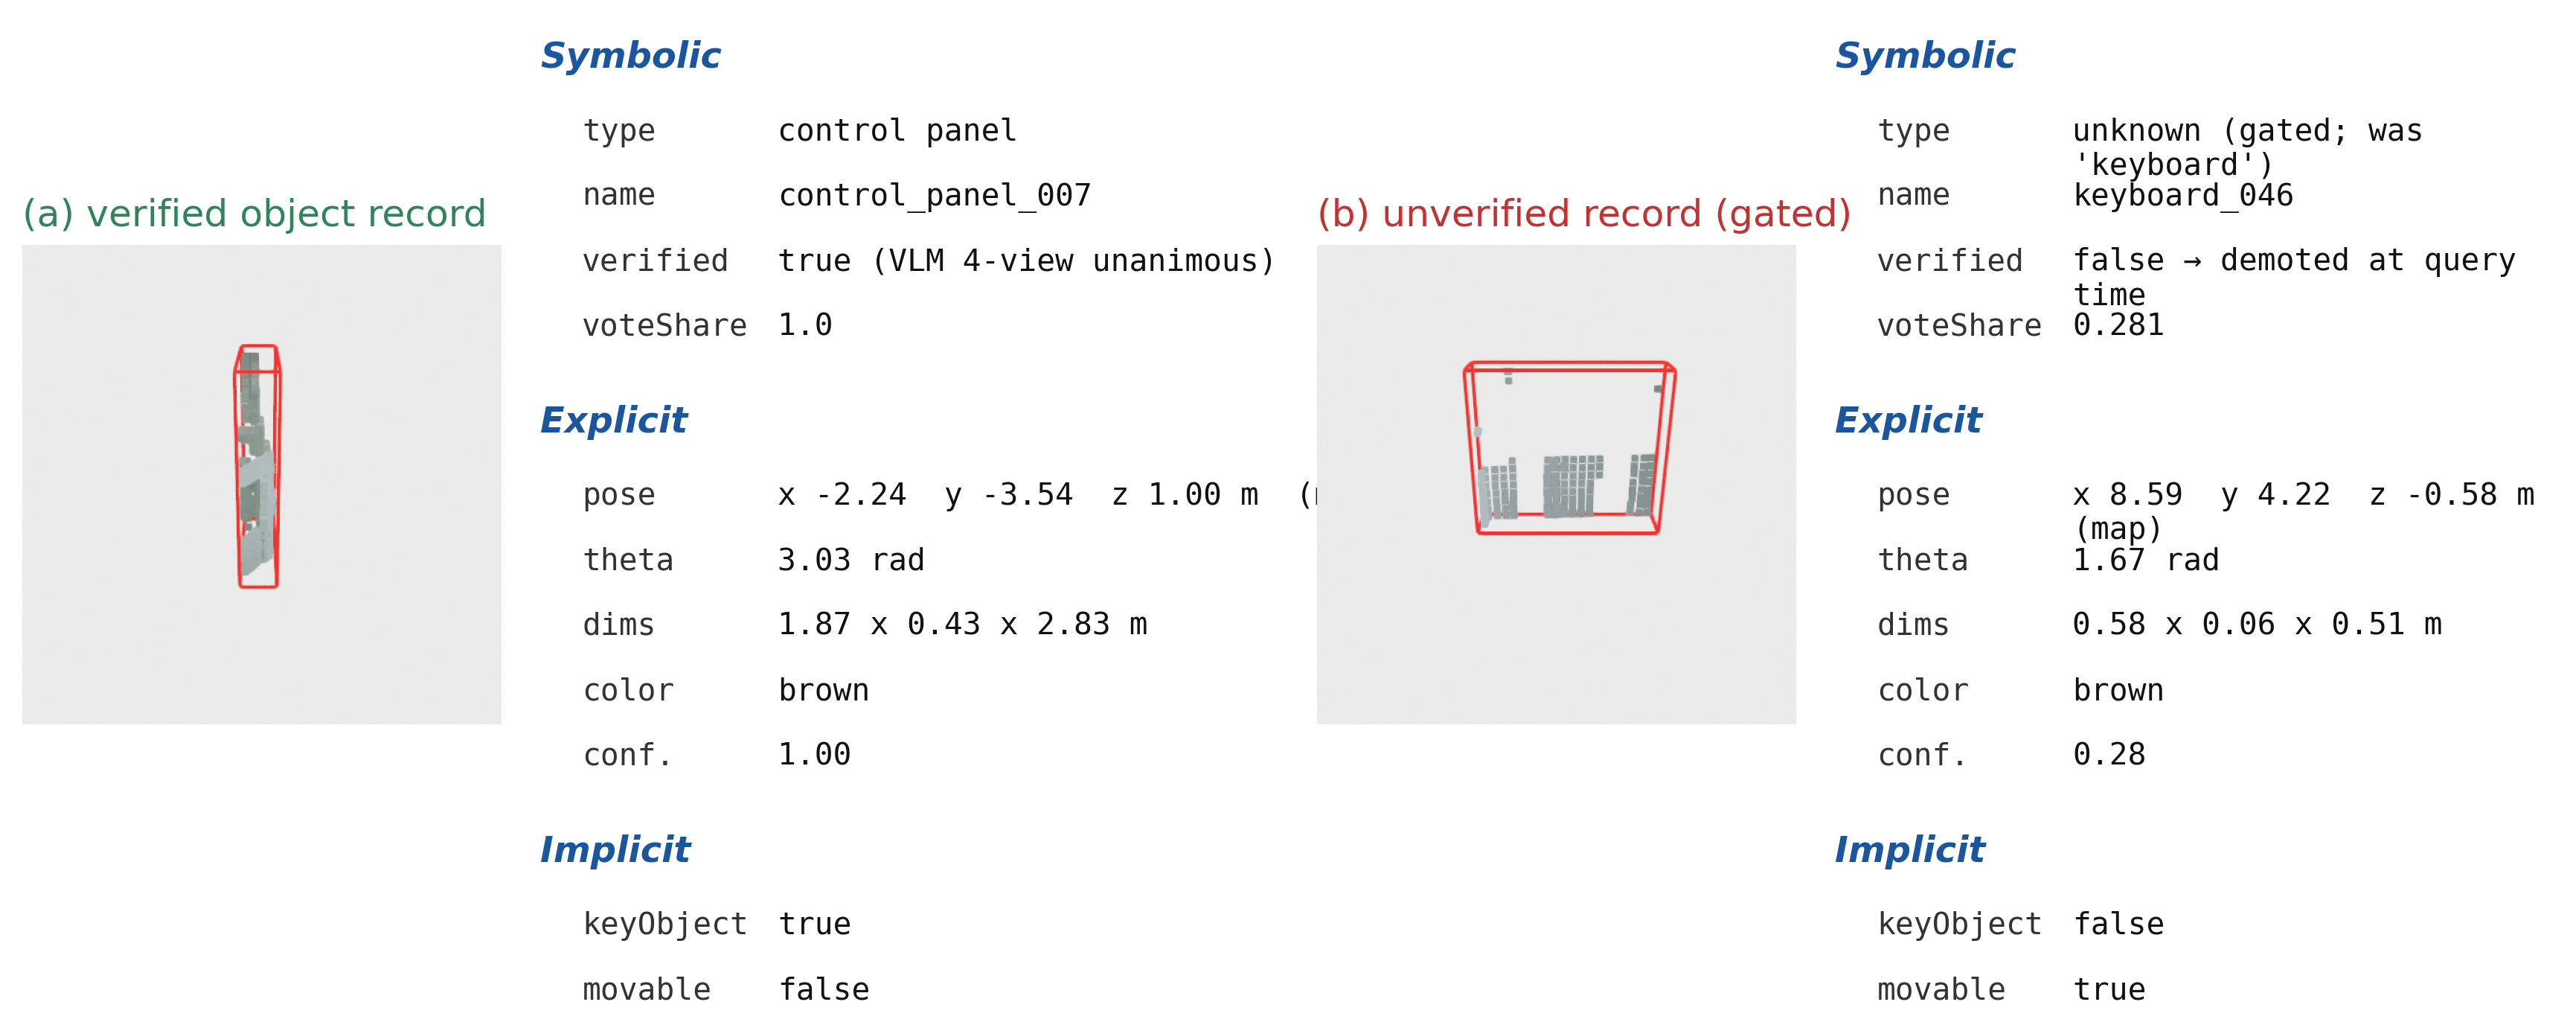
\includegraphics[width=0.95\linewidth]{fig4_record_cards.png}
\caption{TOSM semantic-object records (symbolic / explicit / implicit
layers). (a)~A verified record asserts its type. (b)~An unverified record
is structurally gated at query time: the type is demoted to
\texttt{unknown} and the failed classifier guess is quarantined in
\texttt{failedCandidateType}.}
\label{fig:cards}
\end{figure}

\subsection{Object-Grounded Place Layer}
\label{sec:place}

Robot tasking refers to places (``the docking area'') as often as to objects.
Following the TOSM place schema of DK-SMF~\cite{joo2025dksmf}---boundary
polygon, containment, and purpose---we add a place layer grounded in the
verified object layer. Place regions are obtained automatically from the
robot-facing occupancy grid map (0.05\,m---generated from the scan here,
and equally the exploration SLAM map on deployment), following DK-SMF's
recipe: the room interior delimited by the mapped outer boundary is
partitioned by SLIC superpixel segmentation~\cite{achanta2012slic} with the
number of superpixels as the governing parameter (7 requested here),
fragments below an area threshold (1.5\,m$^2$) are discarded, and each
region's centroid is the moment-based center of its cells (cf. grid-map
room segmentation~\cite{bormann2016room,luperto2022robust}). Each
object's \texttt{isInsideOf} resolves to the region containing its anchor
cell. Each place is then summarized by its
\emph{ring code}: the sequence of member objects sorted by bearing around the
place centroid---restricted to verified-tier objects, so the confidence gate
propagates into place semantics---and a single LLM call names the place from
its ring code. Because the segmentation depends only on the map, region
identity is stable across scan epochs, and the same regions re-derive names
that track the room's actual use (the machine bay: exhibition-era
\texttt{machine\_access\_area} $\rightarrow$ storage-era
\texttt{clutter\_zone} $\rightarrow$ test-era
\texttt{machine\_operator\_station}; Sec.~\ref{sec:exp-update}), demonstrating that place
semantics stay current without manual re-annotation.
Fig.~\ref{fig:placemap} shows the resulting T3 place layer. The robot
layer of TOSM is out of scope here.

\begin{figure}[t]
\centering
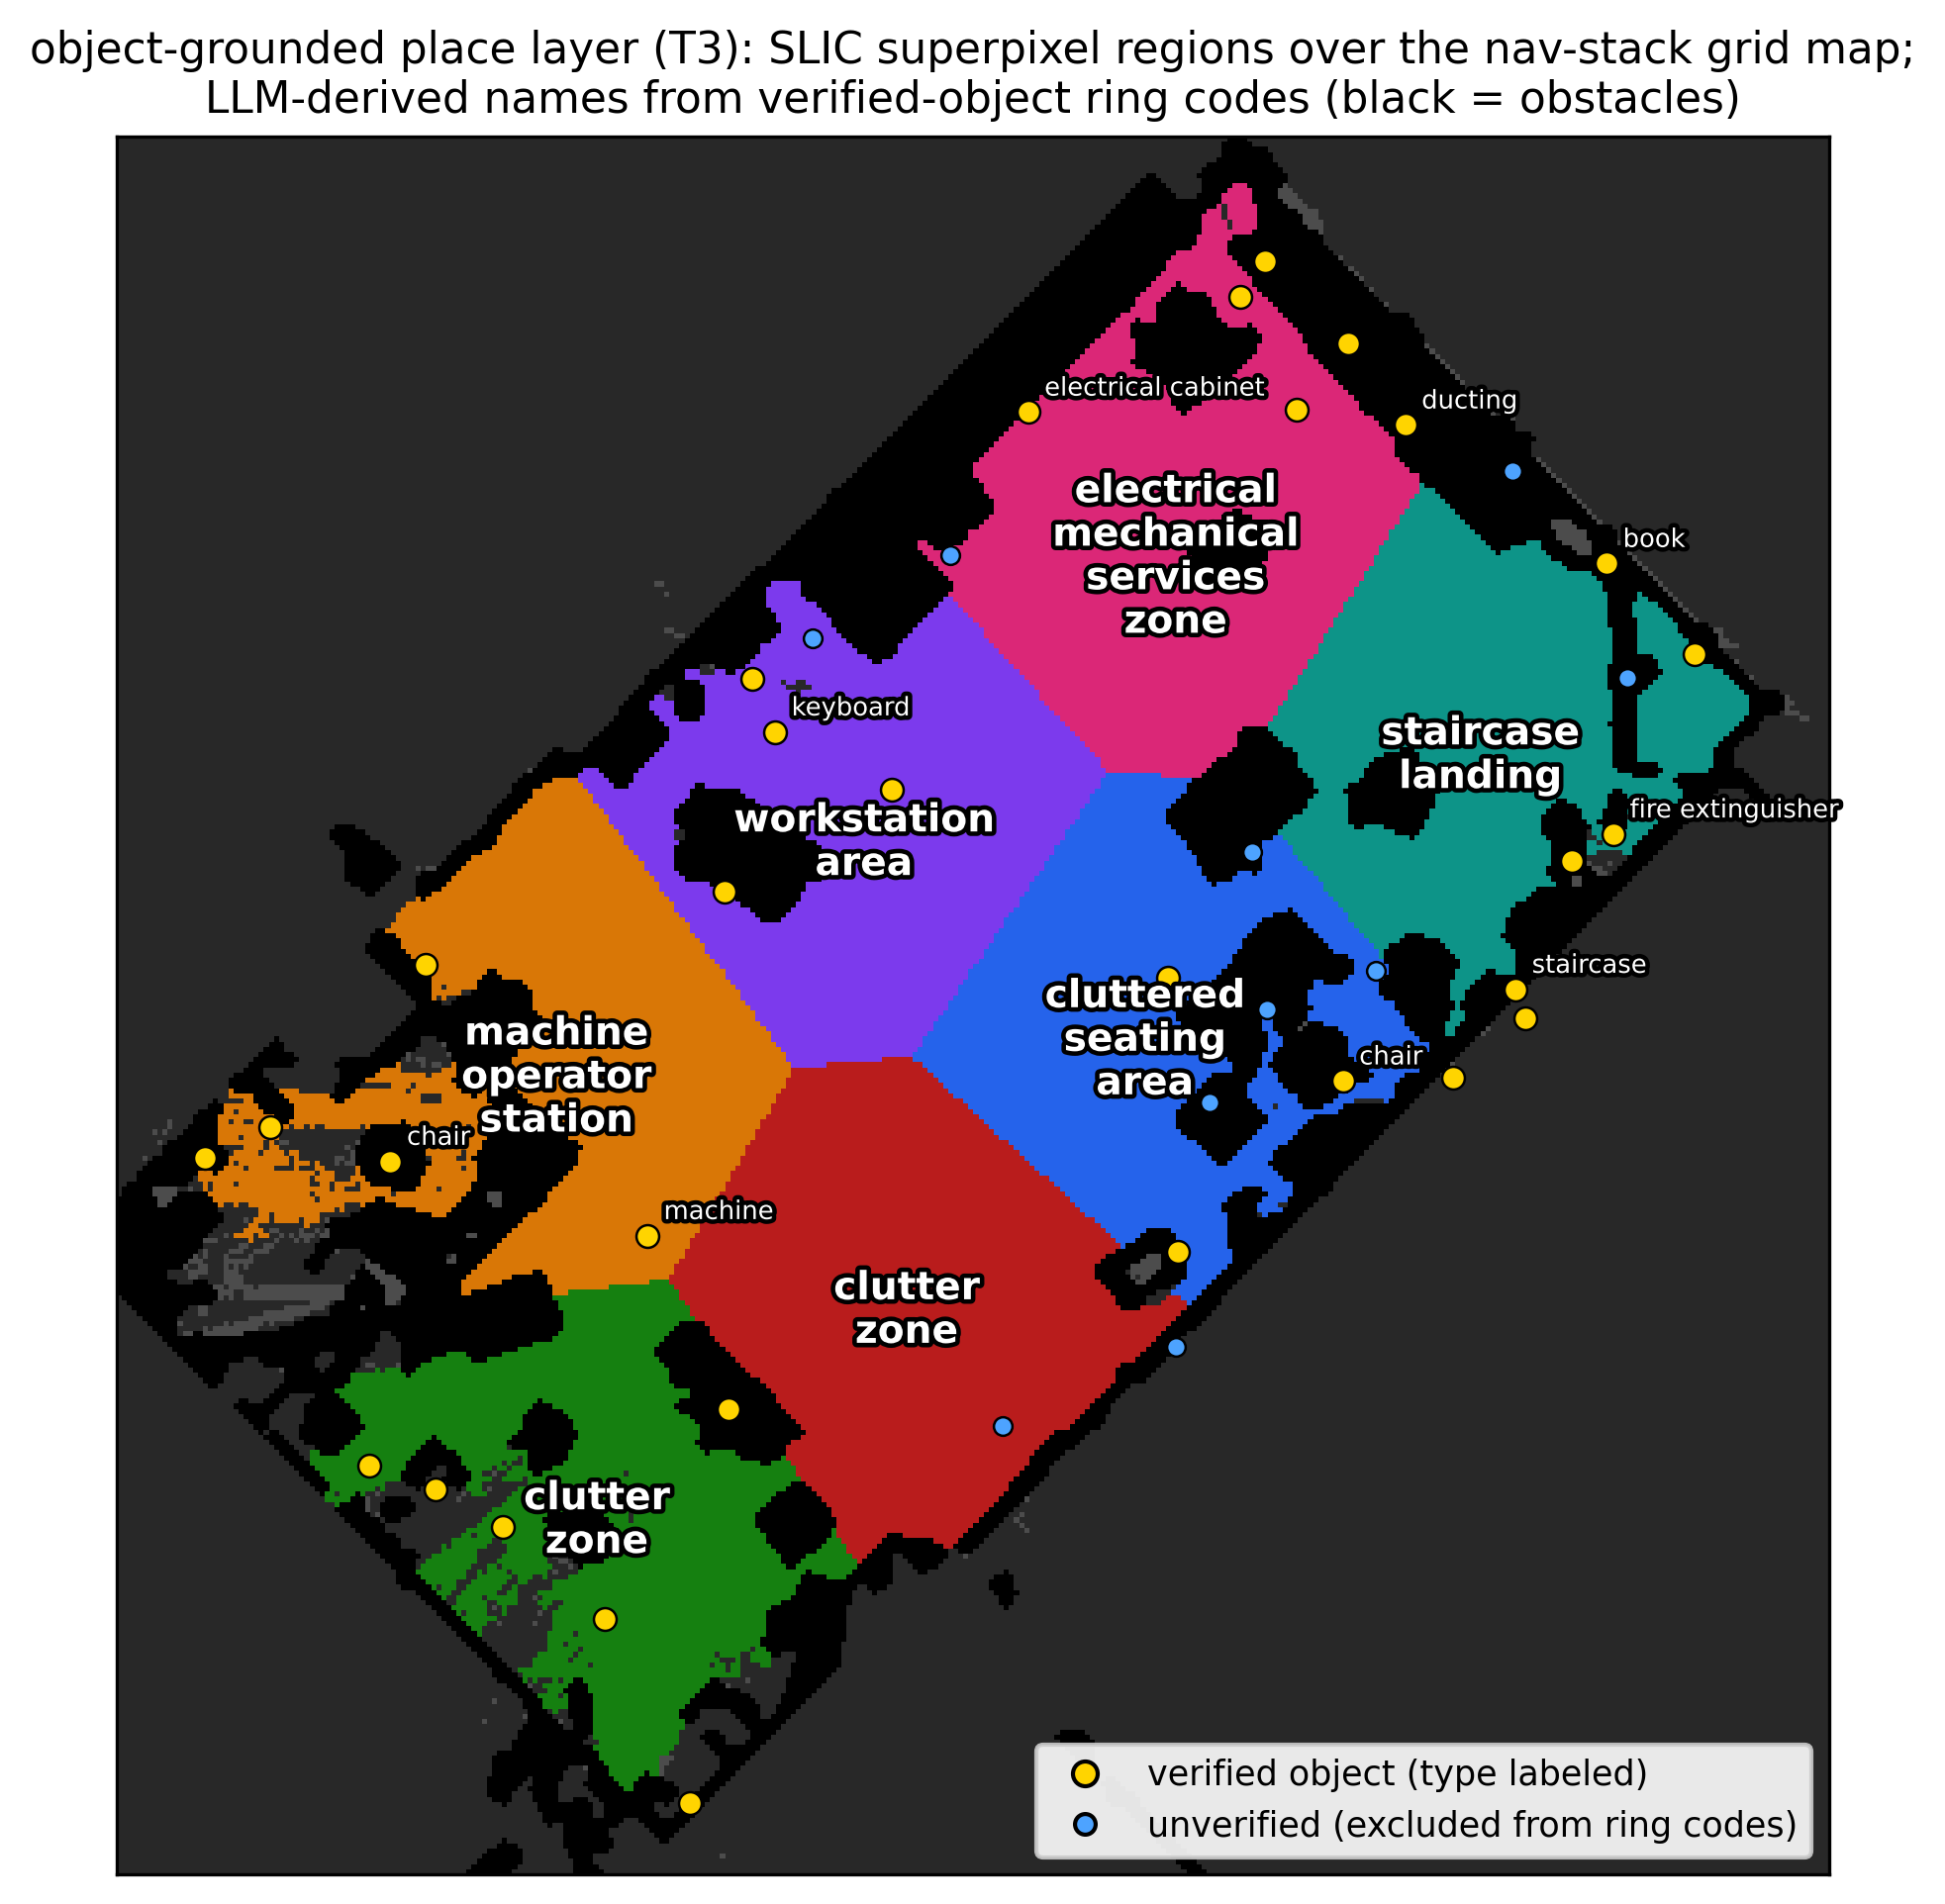
\includegraphics[width=0.85\linewidth]{fig11_place_map.png}
\caption{Object-grounded place layer at T3. SLIC superpixel
regions~\cite{achanta2012slic} tile the room interior delimited by the
nav-stack grid map's outer boundary and carry LLM-derived names computed
from verified-object ring codes; unverified objects (blue markers) do not
contribute, so the confidence gate propagates into place semantics. Shown
at the graph's owner-corrected revision (Sec.~\ref{sec:exp-owner}).}
\label{fig:placemap}
\end{figure}

\section{Experiments}
\label{sec:experiments}

\subsection{Setup}
\label{sec:setup}

\paragraph{Scenes and epochs.}
All main-campaign data comes from BLK360 scans of two industrial indoor
environments that
are, in fact, one room observed across its working life---a property we
exploit deliberately. The \emph{showroom} epoch (June 2026) captures the room
in an exhibition configuration, scanned manually with the door open; its
semantic target is the wall-removed export (38 objects after remnant
filtering). The \emph{robot hall} epoch (July 2026) captures the same room
reorganized as a robot test hall, scanned by autonomous visibility-driven
exploration (81 objects, room-scoped to 55). A third epoch (late July 2026)
adds a controlled-change re-scan at 99.6\% coverage (Sec.~\ref{sec:exp-update}).
Because the two primary epochs differ in layout, furnishing, and scan
modality, they function as independent scenes for per-epoch evaluation
(Secs.~\ref{sec:exp-seg}--\ref{sec:exp-query}) while enabling a real
multi-epoch update study (Sec.~\ref{sec:exp-update}). Scene statistics are
given in Table~\ref{tab:scenes}. A separate scene---a carpeted cafeteria
with sofa booths and vending machines on a different floor of the same
building, scanned in August 2026 (57M points, 28 clusters)---is held out of
the main campaign and used only as a cross-floor, out-of-vocabulary stress
case in Sec.~\ref{sec:exp-ablation}. Both sites are photographed in
Fig.~\ref{fig:photos}.

\begin{figure}[!tp]
\centering
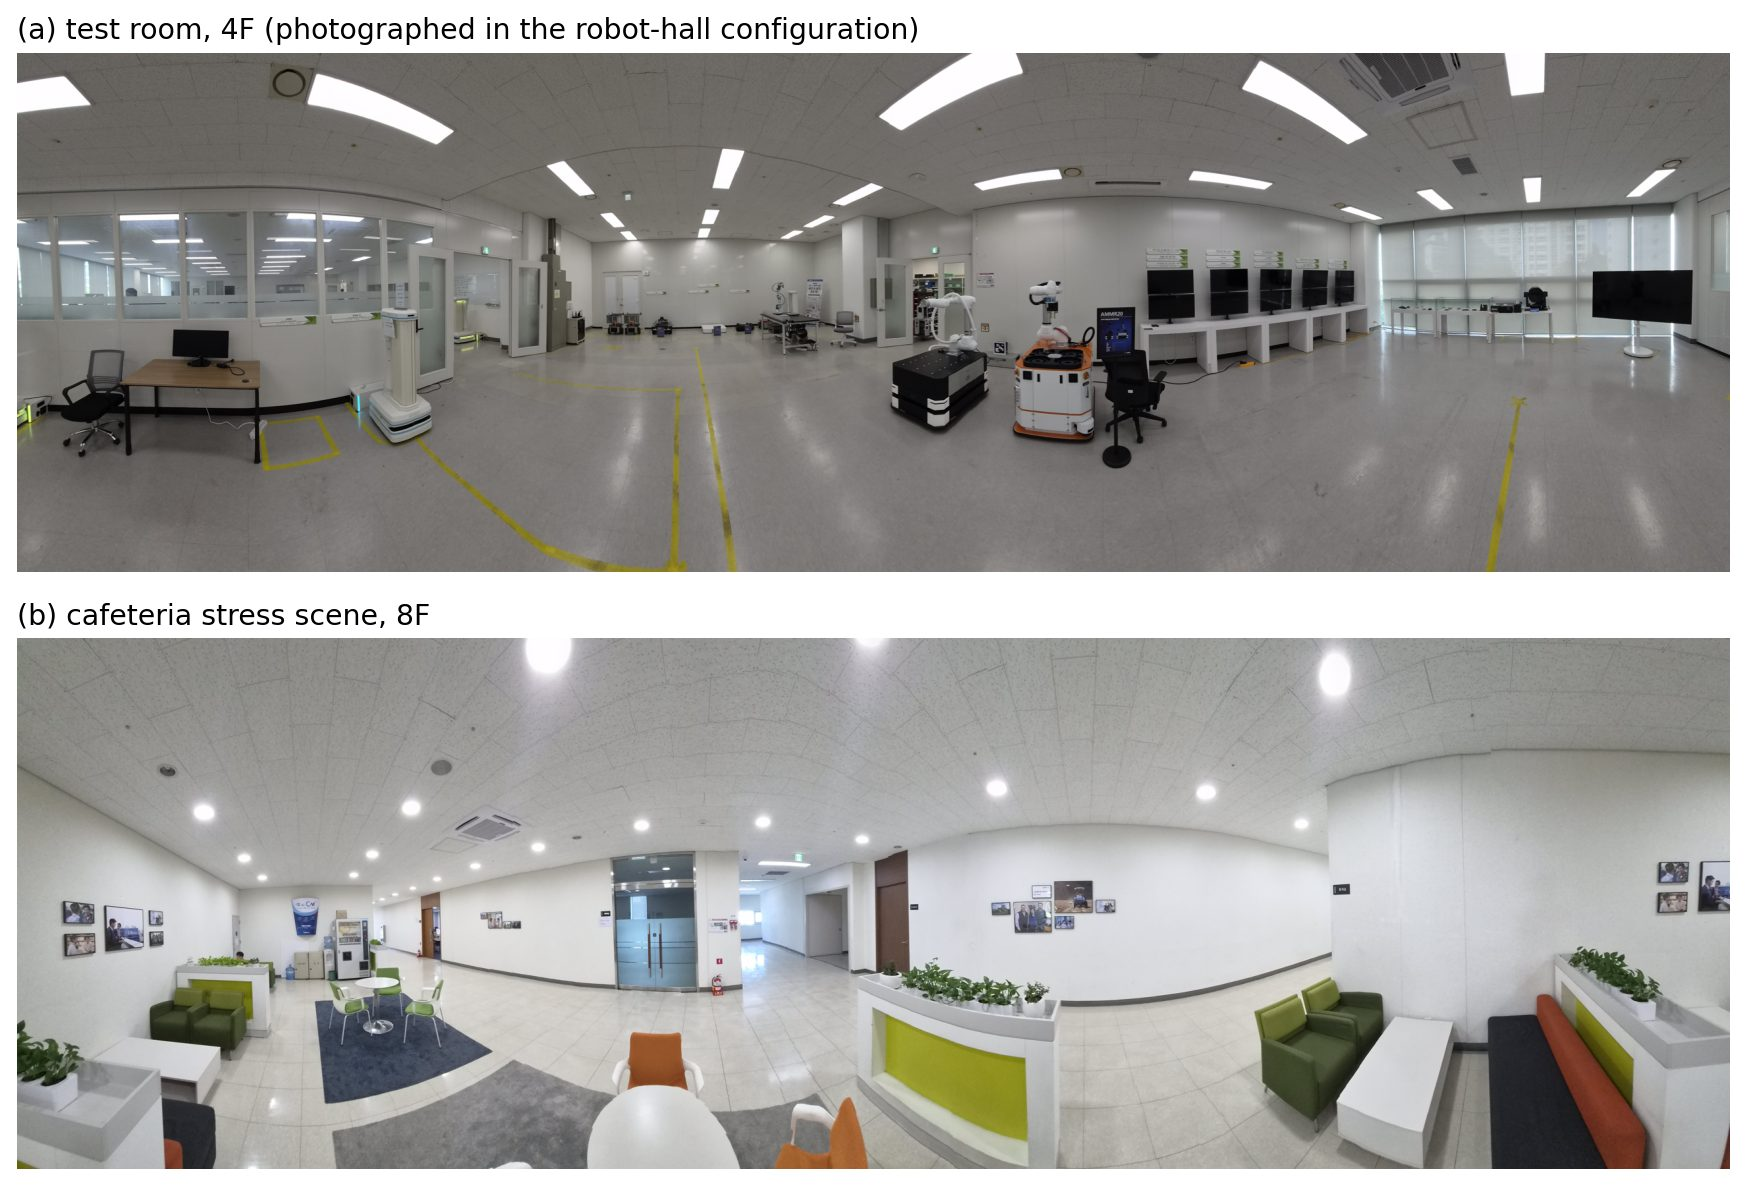
\includegraphics[width=\linewidth]{fig18_scene_photos.jpg}
\caption{The two experimental sites. (a)~The 4F test room, photographed
in its robot-hall configuration (the showroom epoch T1 is an earlier
furnishing of the same room; visible: the AMMR platforms, the
wall-mounted monitor bank of Sec.~\ref{sec:exp-seg}, and the
disinfection robot). (b)~The 8F cafeteria stress scene of
Sec.~\ref{sec:exp-ablation}: fabric sofas, planter partitions, the
vending row, and---center right---the brown door recovered by
escalation on full-resolution renders.}
\label{fig:photos}
\end{figure}

\begin{table}[t]
\centering
\caption{Scene statistics (deterministic detection ``det'' sets, after
structure-remnant filtering).
T1 semantic processing starts from a manually wall-removed export (4.9M
points) of the 46.3M-point raw scan.}
\label{tab:scenes}
\small
\begin{tabular}{@{}lccc@{}}
\toprule
 & Showroom (T1) & Robot hall (T2) & Re-scan (T3) \\
\midrule
Scan mode & manual, 1 setup & exploration & exploration (SOTA), 6 setups \\
Raw points & 46.3M & 68.6M & 70.2M \\
Clean cloud (post-removal) & --- & 267K & 294K \\
Objects (filtered) & 38 & 81 & 79 \\
Room-scoped & 38 & 55 & 41 \\
Removed planes & 10 & 10 & 10 \\
\bottomrule
\end{tabular}
\end{table}

\begin{table}[t]
\centering
\caption{Evaluation-set lineage: how every cluster set used in
Sec.~\ref{sec:experiments} derives from its scan. All counts are
recomputed from the archived stage outputs in the data package;
$\dagger$ marks the one count grounded only in the experiment log.
``conf.''\,=\,GT-confirmed.}
\label{tab:sampleflow}
\footnotesize
\setlength{\tabcolsep}{3.5pt}
\begin{tabular}{@{}ll@{}}
\toprule
Lineage & Stage flow (cluster counts) \\
\midrule
Showroom 57-set (Sec.~\ref{sec:exp-verify}) & 30 pre-split
$\rightarrow$ 57 split $\rightarrow$ 50 after soffit filter
$\rightarrow$ 50 GT-scored (36 conf.) \\
Showroom det set & 45 raw $\rightarrow$ 38 after soffit filter
$\rightarrow$ 38 room-scoped \\
Robot hall det & 88 raw $\rightarrow$ 81 filtered $\rightarrow$ 55
room-scoped $\rightarrow$ 51 GT-scored (32 conf.) \\
T3 det1 & 79 merged $\rightarrow$ 41 room-scoped (= owner audit set)
$\rightarrow$ 26 filter survivors \\
T3 det2 (precut) & 66 $\rightarrow$ 35 room-scoped $\rightarrow$ 27 to
VLM (8 wall sheets excluded) \\
T3 det3/det4 & 33 consolidated $\rightarrow$ 46$^{\dagger}$ adjudicated \\
Cross-epoch KG (present) & rev7$\rightarrow$14:
47, 49, 51, 63, 64, 64, 46, \textbf{46} (current) \\
det5 frozen re-run (Sec.~\ref{sec:exp-endtoend}) & 66 $\rightarrow$ 35
in-room, scored vs.\ the 46-object graph \\
Cafeteria 8F & 28 $\rightarrow$ 25 GT-scored (20 conf.) \\
\bottomrule
\end{tabular}
\end{table}

\paragraph{Ground truth.}
Ground truth was established in two passes: a render-based audit of every
cluster, followed by confirmation from the room's owner. Labels are graded
\emph{confirmed} (owner-verified), \emph{plausible}, or \emph{unknown};
accuracy is reported against confirmed GT (with lenient variants including
plausible where stated), unknown objects are excluded, and structure
artifacts are tracked separately. Two showroom sets must be distinguished:
Table~\ref{tab:scenes} counts the 38-object reproducible det set, while the
verification study (Sec.~\ref{sec:exp-verify}) uses the original 57-cluster
decomposition of the same scan, of which 50 clusters are GT-scored after
excluding 7 structure artifacts---yielding confirmed 36 / plausible 12 /
unknown 2. Table~\ref{tab:sampleflow} connects every evaluation set used
in this section---the 38-object det set, the 50-scored showroom subset,
and the T3 41-, 35-, and 46-object sets---to its derivation stage, so no
denominator has to be inferred from prose. For the room-scoped robot hall (55 objects), GT covers 51
clusters: confirmed 32 (lenient $n{=}42$) after owner corrections. The
cafeteria stress scene follows the same practice: 25 of 28 clusters scored
(3 structure artifacts excluded), confirmed 20 / plausible 5. Both audit
passes share an anchoring channel---the render audit presents proposed
labels that the owner then corrects---so confirmed grades are owner
decisions over physically known rooms rather than blind annotations; the
owner overturned model-favored labels in several cases (a
``refrigerator'' re-graded as a banner, a verified keyboard refuted as a
phantom, ``motors'' re-identified as mobile manipulators), which bounds
but does not eliminate this bias. To measure it directly, a second
annotator---a co-author familiar with the facility who had seen neither
the T3 pipeline output nor the owner audit---labeled all 41 T3 clusters
\emph{blind}, from full-resolution multi-view render sheets carrying only
neutral shuffled IDs, in free vocabulary with a 1--5 confidence. On the
33 clusters both annotators labeled, the blind labels agree with the
owner's on 31 (93.9\%; the two disagreements are low-confidence blind
labels, 2--3/5); the blind annotator abstained on 5 clusters and both
were uncertain on 2. The most informative split for anchoring is by whether the owner had
\emph{overridden} the model: on the 31 clusters where the owner
overturned the pipeline label, the blind annotator independently
reproduced the override on 25 of the 26 it scored (abstaining on 5),
versus 6 of 7 where the owner had accepted the model label. The 25/26 reproduction of the owner's overrides argues against those
corrections being driven primarily by model anchoring; the accepted
subset is small (6/7), so residual anchoring cannot be excluded, and we
therefore describe the owner ground truth as anchoring-bounded rather
than anchoring-free. A third annotation, added for this revision, comes
from an external annotator with no connection to the work and no
familiarity with the facility, who labeled the same 41 sheets blind
under the same protocol. Without site knowledge, agreement with the
owner drops to 21 of the 33 clusters scored (63.6\%; 5 abstentions, 2
both-uncertain), but it is strongly confidence-dependent: 16 of 19
labels given at confidence 4--5 agree (84\%), against 5 of 14 at
confidence $\leq$3, and 11 of the 12 disagreements fall on the two
categories the paper singles out as render-ambiguous --- absorbed or
merged industrial objects (six, e.g.\ the conveyor belt read as a work
table) and ceiling or wall remnants read as floor-level objects (five).
We read the external
result as the honest bound on render-only annotation: distinctive
furniture and robots are labeled consistently by anyone, while the
categories that required on-site knowledge in the owner audit are
exactly those an unfamiliar annotator cannot resolve from renders. The
blind kits, all three answer sheets,
and scoring are in the data package.

\paragraph{Metrics.}
Classification accuracy is top-1 against GT under a documented
synonym-tolerant matching (e.g., \emph{mobile manipulator} $\approx$
\emph{robotic arm}). Verification quality is reported as per-tier precision
(unanimous, escalated, unverified). For query evaluation, a
\emph{hallucination} is an unsupported atomic factual claim, and the rate is
unsupported claims over all factual claims in the answer set. Update quality
uses the metrics of Sec.~\ref{sec:matching}: matching accuracy,
identity-switch rate, false-new, false-absent, and unchanged stability.

\paragraph{Controls.}
The verifier for the main campaign (Secs.~\ref{sec:exp-seg}--\ref{sec:exp-update}) is fixed to a single
model, \texttt{claude-\hspace{0pt}sonnet-\hspace{0pt}4-6} (the frontier
mid-tier at campaign start):
every verification, escalation, and owner interaction in the accumulated
knowledge-graph lineage was produced under this one verifier, so results
remain comparable across sections and revisions. The verifier choice itself
is then evaluated in Sec.~\ref{sec:exp-ablation}, which repeats the
identical Stage-B protocol across five commercial VLMs and re-runs the
headline verification study under the best-ranked one.
All query conditions share the same LLM (\texttt{claude-sonnet-4-6}), system
prompt, query set, decoding parameters, retry policy, and forced answer
schema; conditions differ \emph{only} in the knowledge view they receive.
The LLM-only condition---an \emph{unverified Stage-A LLM} baseline---receives the same scene's Stage-A object dump, so it
is not information-starved---it is verification-starved.
Threshold provenance is stated in two parts. Constants in the base
pipeline (Secs.~\ref{sec:preprocess}--\ref{sec:upsert}) were fixed on
T1/T2 and applied unchanged to T3 and the cafeteria. The corrective-layer
thresholds of Sec.~\ref{sec:corrective} were developed on the test-room
lineage---including failures revealed by the T3 owner audit
(Sec.~\ref{sec:exp-owner})---and were then frozen before evaluation on
the cafeteria stress scene; accordingly, T3 is treated as a retrospective
development-scene replay of those layers rather than a held-out
evaluation (Sec.~\ref{sec:exp-endtoend}). Nothing is trained, so the
split that matters is the development room (T1/T2/T3) versus the
held-out cafeteria, and Sec.~\ref{sec:exp-endtoend} states which claims
survive on which side of it.

\paragraph{Generative AI use.}
Generative models enter this study in two strictly separated roles,
disclosed here per the journal's GenAI policy. As \emph{experimental
components under test}: commercial VLM/LLM services perform Stage-B
multi-view verification (\texttt{claude-sonnet-4-6} throughout the main
campaign; Anthropic PBC, San Francisco, CA, USA), the query-benchmark
answering under all four conditions (the same model), place-name
generation from ring codes, and the five-verifier comparison of
Sec.~\ref{sec:exp-ablation} (Anthropic and OpenAI models); every such
call is made under a forced tool-use schema with prompts, decoding
parameters, model identifiers, and per-call usage archived in the data
package, and these models contributed no text to this article. As a
\emph{writing aid}: a generative AI assistant was used for language
editing and LaTeX formatting of the manuscript, as declared in the
Acknowledgments; it played no role in study design, data collection, or
analysis beyond the archived experimental calls above.

\subsection{Segmentation: Repeatability, Filtering, and Sensitivity}
\label{sec:exp-seg}

\paragraph{Repeatability.}
Running the full pipeline twice from the same E57---including ten-plane
structure removal---reproduces every cluster byte-identically on both
scenes (hash-verified). To probe robustness beyond one software stack, we
packaged the backbone into a version-pinned container and re-ran the
robot-hall scan under a deliberately different environment (glibc 2.41
vs.\ 2.39, Python 3.12.14 vs.\ 3.12.3): all 81 retained clusters remain
byte-identical to the native run, and consecutive container runs
reproduce each other exactly. Running the same container on a second
machine with a different CPU vendor and microarchitecture (Intel Core
i9-13900H laptop vs.\ the AMD Ryzen~9 9900X reference workstation)
reproduces the identical per-cluster checksums and aggregate hash---the
determinism claim therefore holds across operating environments and
x86-64 CPU vendors under the pinned library set. The verification kit
(container recipe,
reference checksums, comparison script) ships with the data package so
the check can be repeated elsewhere; bit-level
reproducibility across instruction-set architectures is not claimed.
This is the property the incremental machinery
builds on: identical clusters mean carryable verification results and
attributable diffs.

\paragraph{Remnant filter.}
The structure-remnant filter of Sec.~\ref{sec:decomposition} removed all
fourteen owner-confirmed ceiling-soffit phantoms (seven per scene: showroom
45$\rightarrow$38, robot hall 88$\rightarrow$81) while leaving every retained
cluster
unchanged. Before the filter, these phantoms did not merely inflate the
object count: they produced confidently verified fictions (keyboard panels,
handrails) that survived multi-view voting, since every view showed the same
wall-colored slab. Detecting structure remnants \emph{geometrically},
upstream of semantics, proved more reliable than asking the verifier to
doubt itself (cf. the pose-context ablation, Sec.~\ref{sec:exp-ablation}).

\paragraph{Parameter sensitivity.}
A 36-combination sweep (giant-split footprint $\times$ DBSCAN
$\varepsilon$ $\times$ minimum points) shows a stable plateau
at footprint 2.0--2.5\,m: instance recall degrades at 3.0\,m as neighbors
merge and at 1.5\,m as equipment shatters, while
$\varepsilon$/min-point extremes collapse recall to 0.21. Because scoring
a sweep against the operating point's own decomposition would be
circular, we re-scored every combination against an independent
object-level reference: the owner-audited inventory, in a
membership-independent form (all clean-cloud points falling inside each
owner-audited oriented box, so no clustering decision defines the
reference). On the robot hall (42 reference objects) the conclusion
survives intact: the min-points-100 band is a broad plateau, and the
operating point (2.5\,m / 0.30 / 100) sits at the grid maximum under
the independent reference (recall 0.952, a uniform $\sim$0.05 below the
cluster-referenced numbers, with the plateau shape unchanged). On the
showroom, the audit surfaced an error we report plainly: the original
showroom sweep rows had joined the reference onto the operating run's
own clusters, and against the genuinely audited 57-object inventory
\emph{no} grid combination of the base clustering exceeds recall 0.33
--- the audited granularity of that scene is produced by the
split-refinement stage, not by any base-DBSCAN setting. The showroom
rows are therefore evidence for the necessity of the refinement stage,
and the parameter-robustness claim rests on the non-circular robot-hall
table (full grids in the data package).

\paragraph{Conditional Point-SAM refinement.}
Under a pre-specified rule (adopt iff $\geq$50\% of merged-cluster failures
separate correctly \emph{and} label accuracy improves $\geq$5 points),
Point-SAM separated 3/6 flagged merged clusters and sub-cluster labels
reached 9/11 versus 5/11 for their parents (+36.4 points,
Fig.~\ref{fig:baselines}), so the rule is met for \emph{flagged merged
candidates}; because automatic candidate selection also produced 2/6
false positives that fragment single objects, Point-SAM is retained only
as an optional, manually triggered diagnostic refinement---it is not part
of the frozen pipeline of Sec.~\ref{sec:corrective} and contributes
nothing to the end-to-end replay of Sec.~\ref{sec:exp-endtoend}.

\begin{figure}[t]
\centering
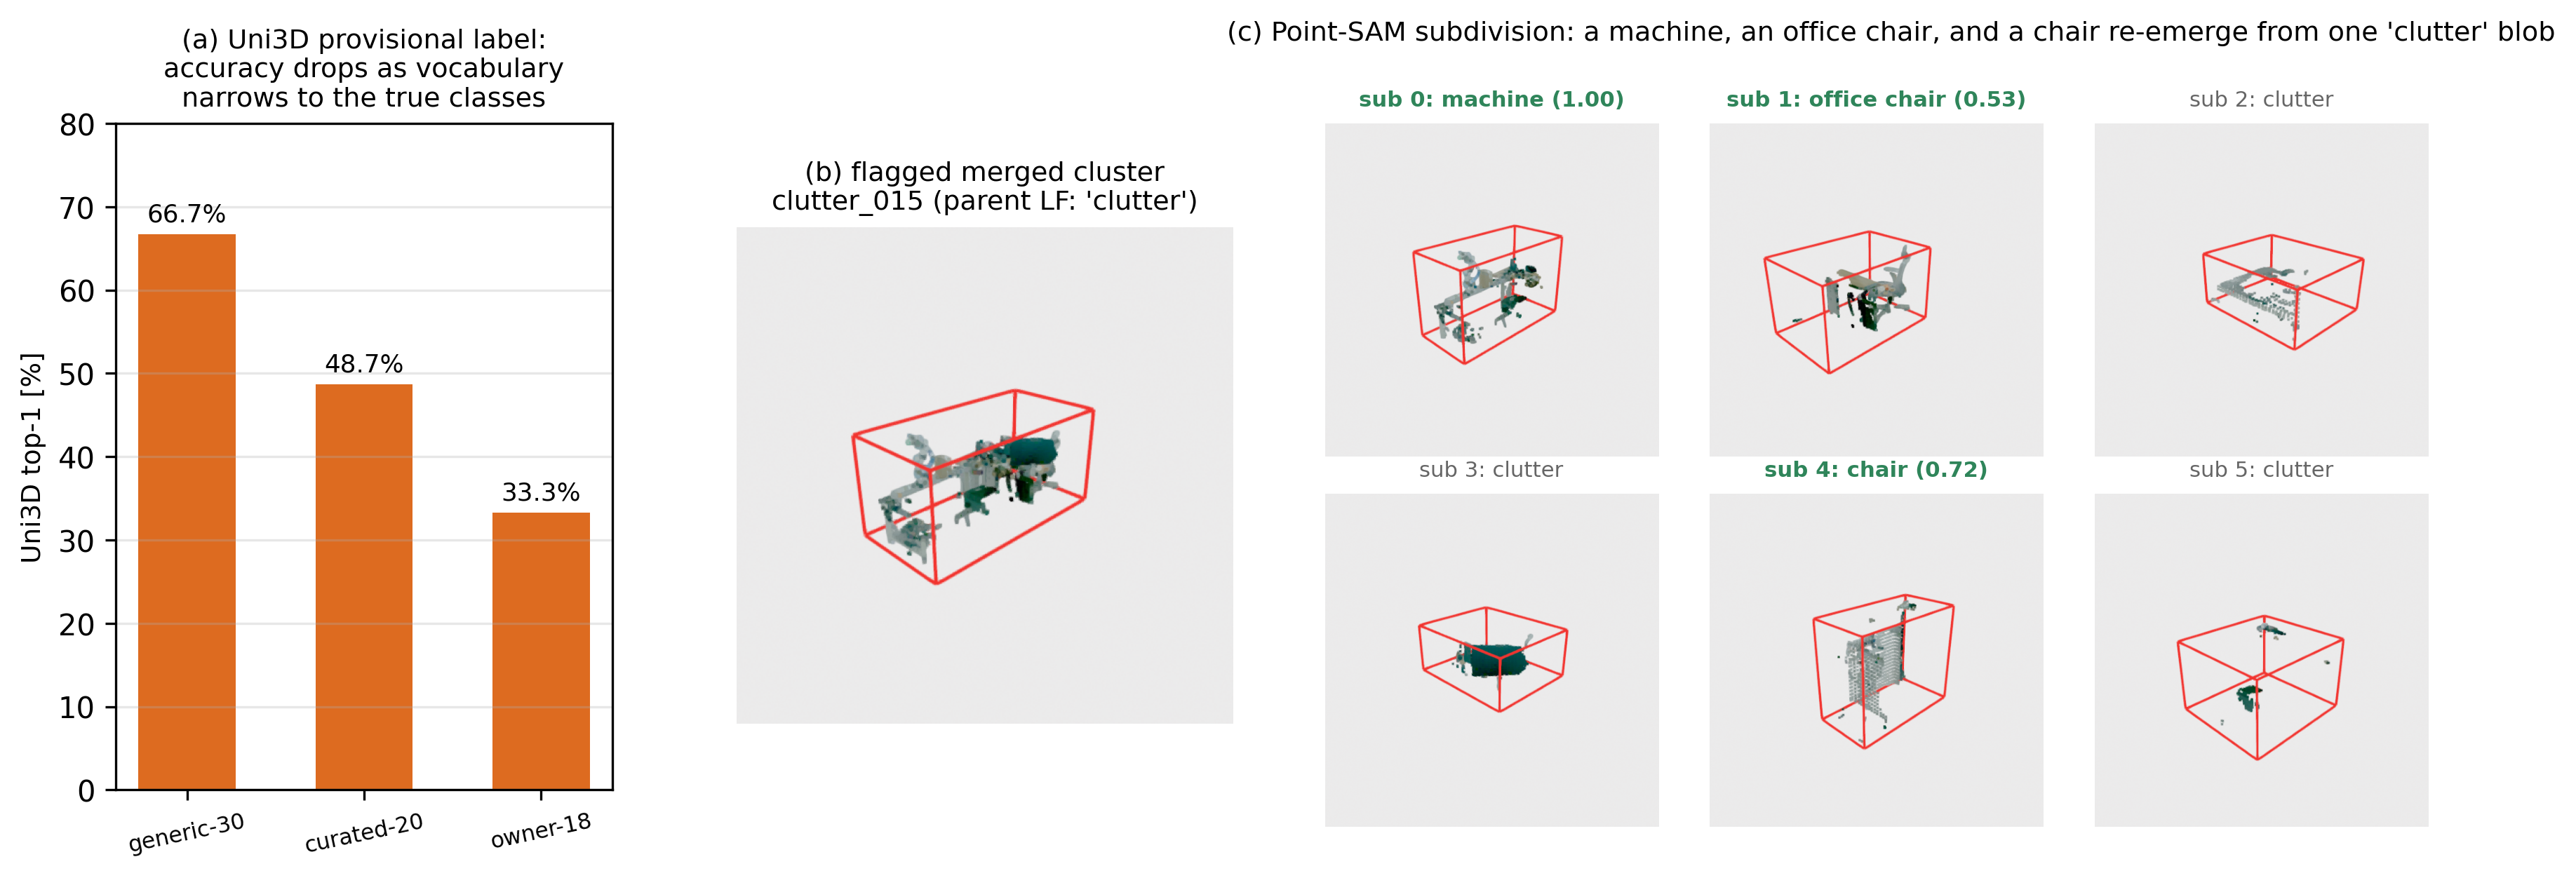
\includegraphics[width=0.95\linewidth]{fig13_pointsam_uni3d.png}
\caption{Learned components used as bounded tools. (a)~The Uni3D provisional
label degrades as the vocabulary narrows to the deployment's true classes
(Sec.~\ref{sec:exp-ablation})---why it is treated as untrusted context.
(b,c)~Conditional Point-SAM refinement of a flagged merged cluster: a
machine, an office chair, and a chair re-emerge from a single
\texttt{clutter} blob, each re-verified independently.}
\label{fig:baselines}
\end{figure}

\paragraph{Coverage stress case.}
The T3 epoch supplied a stress case: at 99.6\% coverage, inter-object
gaps close and DBSCAN chains 120K points (41\% of the clean cloud) into one
$10.4\times9.6$\,m mega-cluster that survives the giant-split. Refinement
recovers little of the resulting diff inflation---of the epoch's 45 absent
nodes, 43 retain a source cluster to re-associate against; Point-SAM
($K{=}7$ prompts) re-associates 4 of these 43, tighter re-splitting
($\varepsilon{=}0.12$) 5 of 43---which is itself informative: $\sim$88\% of
that epoch's absences reflect genuine scene change, not segmentation
artifacts (Sec.~\ref{sec:exp-update}).

\paragraph{Backbone selection.}
The DBSCAN\,+\,Uni3D backbone was chosen against learned alternatives on
a wall-removed industrial scene (122.7K points), summarized in
Table~\ref{tab:backbones}. The metrics are deliberate proxies (no point-level
ground truth exists for this scene): point coverage, the fraction of
objects the open-vocabulary classifier cannot name (a boundary-quality
proxy), and label diversity. ScanNet-pretrained SPFormer hallucinates
furniture on industrial content (67 of 88 instances ``chair'') at half
the coverage; PTv3's closed-set semantic head labels 46\% of a scene
\emph{whose walls were already removed} as \texttt{wall} --- a closed
set cannot abstain; and PointCLIP~V2 collapses to a single class.
The geometric backbone wins not by being smarter but by refusing to
guess: its failure mode is unlabeled coverage, which the verification
and owner layers are built to absorb. Point-SAM enters only as the
conditional refiner above.

\begin{table}[t]
\centering
\caption{Segmentation$\times$classification backbone comparison on a
wall-removed industrial TLS scene. The metrics are screening proxies
(no point-level GT) and do not measure instance quality; the PTv3 row
is a semantic-segmentation head whose outputs are not
instance-comparable with the clustering rows and is included only to
document why closed-set semantic heads were screened out. Instance
quality of the retained backbone is validated independently in
Secs.~\ref{sec:exp-seg} (owner-referenced sweep)
and~\ref{sec:exp-endtoend} (end-to-end recall).}
\label{tab:backbones}
\footnotesize
\setlength{\tabcolsep}{4pt}
\begin{tabular}{@{}lcccl@{}}
\toprule
Pipeline & Coverage & Unnameable & Classes & Dominant failure \\
\midrule
\textbf{DBSCAN + Uni3D} & \textbf{98.3\%} & \textbf{23.3\%} & 13 &
unlabeled coverage \\
SPFormer + Uni3D & 51.1\% & 45.9\% & 9 & furniture bias (chair 67/88) \\
PTv3 (semantic) & --- & --- & 17/20 emitted & 46\% ``wall'' after removal \\
DBSCAN + PointCLIP~V2 & 98.3\% & --- & 1--7 & collapse (pipe 23/30) \\
\bottomrule
\end{tabular}
\end{table}

\paragraph{Diffuseness-gated re-splitting.}
This layer and the next are defined, with triggers and parameters, in
Sec.~\ref{sec:corrective}; here we report what they did.
Two T3 clusters that survived every upstream filter are \emph{diffuse
webs}: 95K and 13K points spread over 80 and 12\,m$^2$ at a 2D occupancy
fill below 0.3, versus 0.5--0.85 for every real object in the scene ---
a clean geometric signature, but one density clustering cannot act on,
because the webs are connected at $\sim$1.8\,cm point spacing at any
usable $\varepsilon$. A two-stage re-split resolves them by \emph{cause}
instead of size: points hugging the exploration-grid wall line (inside
the \emph{room polygon}, so wall-flush furniture survives the test that
free-space masks would fail) are structure noise ($\sim$70\% of the
$\sim$95K-point residual); out-of-room bleed-through accounts for another
7\%; the remainder is re-clustered by occupancy-core erosion and, for
compounds, split at the support plane detected as the $z$-histogram
peak 0.5--0.95\,m above floor. The owner's ground truth for the largest
compound --- ``a robot arm on a desk, part of a mobile robot, wall
noise'' --- is recovered exactly: the arm (consensus-verified), the
desk (slab plus under-desk storage), and the partially scanned mobile
robot, plus three columns and a plant. Applied to a $6.2$\,m
wall-flush cluster that verification had confidently labeled
\texttt{electrical cabinet} (0.83), the same machinery --- wall-band
strip, support plane, then density-valley cuts along the wall in the
panel band --- recovers the owner's inventory at unit granularity:
nine of the ten owner-confirmed monitor units, the desk beneath them,
and, from the off-wall remainder, a wheelchair robot and a single
table leg. Unit boundaries are approximate --- the dark screens return
few points, so the cuts follow density valleys in the surrounding wall
band --- and the result is claimed as unit-level recall, not precise
per-unit segmentation. The gate turns ``too diffuse to be an object''
from a discard decision into a decomposition trigger.

\paragraph{Structure-condition ensemble.}
Structure removal is itself a segmentation parameter: it amputates
wall-flush objects along with the wall. Running the geometric pass
under three removal conditions (none / ceiling only / full) and fusing
the results recovered two multi-metre tables that exist in \emph{no}
single-condition segmentation of the production path --- they appear
only when walls are left in place --- raising in-room recall by four
real objects ($\sim$8\%) as a standalone pass (its incremental gain in
the cumulative stack of Table~\ref{tab:layers} is smaller because the
re-split and wall-compound layers already recover part of the same set). The fusion also quantifies label fragility:
only 10 of 37 re-found objects keep the same label across conditions,
and cross-condition \emph{voting} corrected nothing, because the
verifier's biases are correlated across conditions (both recovered
tables were unanimously mis-verified as conveyor belts in every
condition, while the room's actual conveyor unit stayed
\texttt{clutter} in every condition). The ensemble is therefore used as
a recall tool plus a per-object \texttt{labelStability} attribute that
prioritizes owner review --- not as a label fuser.

\subsection{Verification: Fusion and Escalation}
\label{sec:exp-verify}

\begin{table}[t]
\centering
\caption{Verification accuracy against confirmed GT, and per-tier precision.
Accuracy rows are over confirmed GT ($n{=}36$/$32$); trigger rates and tier
counts are over all GT-scored clusters (50 showroom / 51 robot hall), so,
e.g., 21 unanimous $+$ 29 split $=$ 50.}
\label{tab:verification}
\small
\begin{tabular}{@{}lcccc@{}}
\toprule
 & \multicolumn{2}{c}{Showroom ($n{=}36$)} & \multicolumn{2}{c}{Robot hall ($n{=}32$)} \\
 & base-4 & escalated & base-4 & escalated \\
\midrule
Accuracy & 77.8\% & \textbf{88.9\%} & 78.1\% & \textbf{84.4\%} \\
95\% Wilson CI & 61.9--88.3 & 74.7--95.6 & 61.2--89.0 & 68.2--93.1 \\
Recovered / regressed & \multicolumn{2}{c}{5 / 1} & \multicolumn{2}{c}{3 / 0} \\
Escalation trigger & \multicolumn{2}{c}{58\% (29/50)} & \multicolumn{2}{c}{51\% (26/51)} \\
\midrule
Unanimous precision & \multicolumn{2}{c}{100\% (19/19; 21 unan.)} & \multicolumn{2}{c}{94.4\% (17/18; 25 unan.)} \\
Escalated precision & \multicolumn{2}{c}{100\%} & \multicolumn{2}{c}{88.9\%} \\
Unverified precision & \multicolumn{2}{c}{60\%} & \multicolumn{2}{c}{40\%} \\
\bottomrule
\end{tabular}
\end{table}

Escalation lifts confirmed-GT accuracy from 77.8\% to 88.9\% on the showroom
and from 78.1\% to 84.4\% on the robot hall (lenient: 76.2\%
$\rightarrow$ 83.3\%, $n{=}42$), recovering 5 and 3 split-vote objects while
regressing 1 and 0---a consistent observed improvement across both
configurations, though at these sample sizes the paired contrast does not
reach conventional significance (exact McNemar on recovered/regressed:
$p{=}0.219$ and $p{=}0.25$), which the Wilson intervals of
Table~\ref{tab:verification} make explicit (Table~\ref{tab:verification};
Fig.~\ref{fig:esccost} shows the accuracy--cost trade-off at
$\sim$\$0.009/call; escalation adds 232 and 208 calls per scene). The tier
structure
justifies gating: unanimous and escalated tiers reach 88.9--100\% precision,
while the unverified residue is 40--60\%---exactly the content the query
interface must demote. These precision figures are scoped to confirmed
GT: on the showroom, one unanimous vote falls on a \emph{plausible}-graded
cluster and is wrong there (a suspected mobile robot absorbed as
\texttt{clutter}), so the tier's precision over confirmed$+$plausible GT is
20/21 rather than 19/19---the scoping convention is reported so that the
headline is not read as a general property of unanimity (the stress scene
of Sec.~\ref{sec:exp-ablation} degrades it substantially). A repeat of the showroom run under identical
settings bounds the verifier's run-to-run variance: base-4 accuracy
reproduces exactly (77.8\%), escalated accuracy shifts by a single object
(86.1\% vs.\ 88.9\%), the trigger rate by two points (60\% vs.\ 58\%), and
unanimous and escalated precision hold at 100\% in both runs---a
$\pm$3-point scale against which the verifier comparisons of
Sec.~\ref{sec:exp-ablation} should be read. A separate check evaluates the room-scoped T1 objects
in the update-study frame (Sec.~\ref{sec:exp-update}), where showroom GT is
transferred to the re-decomposed clusters by bidirectional point overlap;
on the resulting small confirmed set ($n{=}8$), verified-tier precision is
100\% with 7/7 unanimity.

Verification yield tracks scan quality: the manual scan leaves 47\% of
objects unverified versus 24\% for exploration scans, and re-processing the
T3 scan from a single setup (1/6 coverage) drops the verified tier from
75.6\% to 56.6\% on identical geometry. Coverage buys verifiability.

\paragraph{Per-tier recall.}
Precision alone understates what gating costs, so
Table~\ref{tab:tierrf} completes the tier picture with recall and $F_1$
against confirmed GT. The pattern is consistent: the combined verified
tier reaches recall 0.722/0.781 on the two industrial scenes
($F_1$ 0.839/0.847) but only 0.250 on the cafeteria, where the gate
abstained on half of the confirmed objects---the stress scene's
segmentation failures surface here as recall, not as precision. The
escalated tier is small everywhere (recall 0.194--0.250), consistent
with its role as a recovery channel rather than a primary path.

\begin{table}[t]
\centering
\caption{Per-tier precision, recall, and $F_1$ on confirmed ground truth
(synonym-tolerant). Recall counts a confirmed object as retrieved only if
the tier contains it with the correct type; the unverified row is the
abstention tier, so its ``precision'' is only the fraction of abstained
objects whose withheld top vote happened to be correct.}
\label{tab:tierrf}
\footnotesize
\setlength{\tabcolsep}{3.5pt}
\begin{tabular}{@{}llrrrrr@{}}
\toprule
Scene & Tier & $n$ & $n_{\mathrm{conf}}$ & Prec. & Rec. & $F_1$ \\
\midrule
Showroom & verified (unanimous) & 21 & 19 & 1.000 & 0.528 & 0.691 \\
 & verified\_escalated & 8 & 7 & 1.000 & 0.194 & 0.326 \\
 & combined verified & 29 & 26 & 1.000 & 0.722 & 0.839 \\
 & unverified (abstained) & 21 & 10 & 0.600 & 0.167 & 0.261 \\
 & \emph{confirmed GT total} & 50 & 36 & & & \\
\midrule
Robot hall & verified (unanimous) & 25 & 18 & 0.944 & 0.531 & 0.680 \\
 & verified\_escalated & 16 & 9 & 0.889 & 0.250 & 0.390 \\
 & combined verified & 41 & 27 & 0.926 & 0.781 & 0.847 \\
 & unverified (abstained) & 10 & 5 & 0.400 & 0.062 & 0.108 \\
 & \emph{confirmed GT total} & 51 & 32 & & & \\
\midrule
Cafeteria & verified (unanimous) & 8 & 7 & 0.571 & 0.200 & 0.296 \\
 & verified\_escalated & 6 & 3 & 0.333 & 0.050 & 0.087 \\
 & combined verified & 14 & 10 & 0.500 & 0.250 & 0.333 \\
 & unverified (abstained) & 11 & 10 & 0.200 & 0.100 & 0.133 \\
 & \emph{confirmed GT total} & 25 & 20 & & & \\
\bottomrule
\end{tabular}
\end{table}

\paragraph{Threshold sensitivity.}
Because the 0.6 share threshold gates status only
(Sec.~\ref{sec:verification}), its effect can be quantified exactly by
re-scoring the stored votes at alternative thresholds---no new verifier
calls. Sweeping 0.40--0.90 in steps of 0.05 shows 0.6 sitting on a
plateau rather than a cliff. On the showroom, thresholds 0.55 and 0.60
produce identical tiers (escalated-tier precision 100\%); lowering to
0.50 trades combined verified-tier precision (1.000\,$\rightarrow$\,0.966)
for recall (0.722\,$\rightarrow$\,0.778), and raising to 0.70 keeps
precision saturated while dropping recall to 0.639. The robot hall
behaves the same way (at 0.60: escalated precision 0.889, recall 0.781;
at 0.70: precision 1.000, recall 0.688), and on both industrial scenes
F1 is maximized on a broad 0.45--0.65 band with every 0.05 step moving
at most one or two objects. The stress scene shifts the whole curve
downward without changing its shape---the threshold cannot repair
render- or segmentation-level failures
(Sec.~\ref{sec:exp-ablation})---which is the scene dependence noted for
the tiers themselves. Between 0.50 and 0.70 only 11/34, 12/49, and 7/19
escalated objects change tier on the three scenes, and those bands mix
correct and incorrect labels almost evenly, which is why no alternative
threshold dominates 0.6 by more than single-object noise. We therefore
retain the a-priori 0.6 rather than tuning it post hoc.

\paragraph{Error taxonomy.}
Four recurring error classes emerged (Fig.~\ref{fig:taxonomy}):
(a) \emph{structure-remnant phantoms}---soffit bands verified as keyboards;
eliminated upstream by the remnant filter;
(b) \emph{unanimous-but-wrong}---a hanging chain unanimously verified as a
door handle; an escalated keyboard the owner refuted; partition fragments as
chairs; at T3, a residual $7.4$\,m wall segment that survived the remnant
filter was escalation-verified as a staircase---owner-refuted (``just the
wall'')---and its phantom label then propagated into a place name
(\texttt{staircase\_landing}, Sec.~\ref{sec:place}), showing that place
naming is verifier-bounded too and that wall-scale remnants can slip past a
filter tuned for ceiling-soffit bands (cf. Sec.~\ref{sec:discussion}).
The same propagation reaches the relation layer: a keyboard verified at
full confidence in a room that contains no keyboard (owner-refuted) had
been auto-designated its place's key object before the refutation demoted
it---key-object designation therefore honors owner feedback
(Sec.~\ref{sec:upsert}). A third refutation is the mirror image: the
room's large wall-mounted TV was geometrically detected
(\texttt{monitor\_006}, $2.5\times1.8$\,m) yet left \texttt{unverified}
at 0.26 confidence, while a small co-located cluster was
escalation-verified as a fire extinguisher (0.72) the owner refuted---the
salient real object failed the gate a phantom passed.
Unanimity is strong evidence, not proof, and the gate inherits the
verifier's blind spots;
(c) \emph{clutter absorption}---a disassembled robot, a poster stand, and a
low-reflectance floor fan (674 points) each unanimously verified as
\texttt{clutter}: geometrically detected, semantically flattened;
(d) \emph{render ambiguity} $\rightarrow$ \texttt{unverified}, the intended
failure mode.
Classes (b) and (c) motivate reporting verification as \emph{tiered
evidence} rather than truth, and drive the structural gating design.

\paragraph{Class-level breakdown.}
Table~\ref{tab:classdist} disaggregates every scene's ground truth into
class families and per-family verification outcomes, making the error
classes above quantitative. Three patterns stand out. First, the
vocabulary gap is class-structured: robots are the worst family
everywhere they occur (0/4, 0/3, and 0/8 correct across the three
robot-bearing sets)---absorption, not misperception, since most land in
\texttt{clutter} or abstain. Second, displays and fixtures abstain
heavily on the showroom (0/5 and 0/6 correct, all withheld or
mislabeled)---flat panels and ceiling fixtures are exactly the
render-ambiguous shapes the taxonomy predicts. Third, the T3 owner audit
shows the same distribution end-to-end (6 correct / 25 wrong / 10
abstained over 41), confirming that per-family results, not the
aggregate, are the actionable signal for vocabulary and geometry work.

\begin{table}[t]
\centering
\caption{Ground-truth object classes per scene, grouped into families,
with each object's verification outcome in the canonical run
(synonym-tolerant matching as in the escalation analysis). ``Filtered''
= excluded before scoring (structure artifact or out of room scope).
For the T3 owner audit, correctness follows the owner's category
labels; one verified cluster with no owner answer is counted as wrong
in the total row only.}
\label{tab:classdist}
\footnotesize
\setlength{\tabcolsep}{3.5pt}
\begin{tabular}{@{}llrrrrr@{}}
\toprule
Scene & Family & GT & Corr. & Wrong & Unver. & Filt. \\
\midrule
Showroom (57-set) & seating & 5 & 4 & 1 & 0 & 0 \\
 & robots & 4 & 0 & 1 & 3 & 0 \\
 & displays/monitors & 5 & 0 & 0 & 5 & 0 \\
 & machines/electrical & 6 & 3 & 0 & 3 & 0 \\
 & furniture & 2 & 0 & 0 & 2 & 0 \\
 & fixtures & 6 & 0 & 0 & 6 & 0 \\
 & structure-noise & 7 & 0 & 0 & 0 & 7 \\
 & clutter/unknown & 22 & 20 & 0 & 2 & 0 \\
 & \emph{total} & 57 & 27 & 2 & 21 & 7 \\
\midrule
Robot hall (det) & seating & 5 & 4 & 0 & 1 & 0 \\
 & robots & 3 & 0 & 1 & 2 & 0 \\
 & displays/monitors & 1 & 0 & 0 & 0 & 1 \\
 & machines/electrical & 1 & 0 & 0 & 0 & 1 \\
 & furniture & 2 & 0 & 0 & 0 & 2 \\
 & fixtures & 8 & 3 & 1 & 4 & 0 \\
 & structure-noise & 8 & 0 & 0 & 1 & 7 \\
 & clutter/unknown & 53 & 25 & 7 & 2 & 19 \\
 & \emph{total} & 81 & 32 & 9 & 10 & 30 \\
\midrule
Cafeteria & seating & 10 & 1 & 4 & 5 & 0 \\
 & machines/electrical & 1 & 1 & 0 & 0 & 0 \\
 & furniture & 1 & 0 & 1 & 0 & 0 \\
 & fixtures & 5 & 0 & 1 & 4 & 0 \\
 & structure-noise & 3 & 0 & 0 & 0 & 3 \\
 & clutter/unknown & 8 & 4 & 2 & 2 & 0 \\
 & \emph{total} & 28 & 6 & 8 & 11 & 3 \\
\midrule
T3 re-scan (owner GT) & seating & 5 & 2 & 2 & 1 & 0 \\
 & robots & 8 & 0 & 6 & 2 & 0 \\
 & displays/monitors & 2 & 0 & 1 & 1 & 0 \\
 & machines/electrical & 4 & 0 & 4 & 0 & 0 \\
 & furniture & 4 & 0 & 3 & 1 & 0 \\
 & fixtures & 4 & 0 & 2 & 2 & 0 \\
 & structure-noise & 9 & 0 & 6 & 3 & 0 \\
 & clutter/unknown & 5 & 4 & 0 & 0 & 0 \\
 & \emph{total} & 41 & 6 & 25 & 10 & 0 \\
\bottomrule
\end{tabular}
\end{table}

\subsection{Owner Audit and Corrective Feedback (T3)}
\label{sec:exp-owner}

The preceding subsection measured what the pipeline believes; this one
measures what the room's occupant knows, and how that knowledge feeds
back into the graph. It exercises the revision and upsert machinery ahead
of its formal evaluation (Sec.~\ref{sec:exp-update}); only the feedback
mechanics matter here.

\paragraph{Exhaustive audit and mitigations.}
The room occupant exhaustively labeled all 41 T3 clusters, giving a
distinct T3 owner-audited ground-truth set beyond the showroom scoring
sets.
Of the 31 verified-tier clusters, 6 were correct, 13 were real objects
flattened to \texttt{clutter}, 6 were structure-noise phantoms, 2 carried
a wrong specific label, and 3 were multi-object merges (one unanswered).
The absorption cause is now identifiable: the room is a robotics testbed
(mobile robots, manipulators, charging stations, a disinfection robot),
and none of these classes exist in the classifier vocabulary. The
unverified tier behaved as designed in five structure/fixture cases but
also withheld three real objects, including the wall TV of
Sec.~\ref{sec:exp-verify}. Three audit-driven mitigations follow; their
definitions, triggers, and parameters are given in
Sec.~\ref{sec:corrective} (layers 4--5), and this subsection reports their
development-time evaluation.
\emph{(i) Hybrid structure filter:} registering every cluster against the
exploration-scan occupancy grid --- an independent, drift-free wall prior
--- and combining a wall-line hug test with local (per-metre-segment)
sheet thickness, a full-height band rule ($z$-span $>2.5$\,m), a ceiling
band, and a room-polygon outside test removes structure noise at 12/12
recall with 3 false positives (thin wall-flush real objects: a cabinet
leg, a poster stand). Crucially, the wall-flush monitor bank survives:
its wall-hug fraction is 99\% (the grid map draws it as wall), but its
1.8\,m height and per-segment depth separate it from the 3.2\,m
floor-to-ceiling wall band that plane removal missed. All seven verified
structure phantoms --- the six structure-noise cases above plus a
fluorescent fixture verified as a keyboard at 3.3\,m (audited as a wrong
label) --- are eliminated upstream.
\emph{(ii) Recovery re-verification:} re-asking the verifier with
\texttt{clutter} treated as \emph{unidentified} plus a candidate
shortlist recovered 4 specific types at 4/5 precision with 12 honest
keeps; injecting site vocabulary (robot classes) as candidates doubled
recovery (9 correct) but halved precision (8 wrong) through candidate
anchoring --- the TV became a ``conveyor belt'' when the shortlist ranked
it first. \emph{(iii) Agreement gating:} adopting a recovered label only
when both passes agree, or when a pass agrees with the cluster's own
base label, yields five adoptions at 5/5 precision (two chairs, an
office chair, a machine, and the TV) and resurrects no owner-refuted
phantom. Domain knowledge helps recall; only agreement makes it safe.
Fig.~\ref{fig:structfilter} shows the filter's effect on the T3 epoch.
Regression on the other epochs (no ground truth, manual inspection)
flags 8/50 T1 and 18/55 T2 clusters --- dominated by the documented
soffit phantoms (keyboards, chairs at 2.4\,m, a stair at 3.4\,m) and a
cluster the classifier itself had named \texttt{wall} --- while every
door, chair, machine, elevator, and wall-mounted control panel survives;
the one systematic casualty is a closed-door fragment lying in the wall
plane, consistent with the door-detection asymmetry of
Sec.~\ref{sec:discussion}. Finally, refutations, corrections, and
adopted labels are applied as a fourth KG revision through the same
upsert history mechanism as a rescan: eight phantoms leave the graph,
the poster stand is corrected in place, five recovered types land, the
TV becomes its region's key object, and the relation layer sheds nine
noise-anchored edges (25 to 16 intra-place). Re-deriving ring codes and
names from the revised graph heals the place layer end-to-end: the
phantom-derived \texttt{staircase\_landing} becomes
\texttt{display\_briefing\_area} (TV + poster stand), the
keyboard-derived \texttt{workstation\_area} becomes
\texttt{machine\_area}, and the seating region's recovered chairs turn
\texttt{cluttered\_seating\_area} into \texttt{seating\_area} ---
owner feedback propagates through all three layers of the model: object,
relation, and place.

\paragraph{Feedback at scale: bidirectional, corrective, and
time-variant.}
Extending the audit loop through nine further KG revisions shows owner
feedback operating in all four directions the model supports.
\emph{Restoration}: an object the owner had refuted as absent was later
declared present again (the room changed between audits); a
color-seeded carve at the owner-given corner recovered a 319-point red
cylinder that two-pass verification typed \texttt{fire extinguisher}
(0.72) --- the original failure was segmentation (never proposed), not
classification, and owner ground truth is itself \emph{time-variant},
which is why feedback is recorded as highest-trust evidence with
history rather than as immutable truth. \emph{Refutation}: a
raw-condition ensemble find was refuted as wall paint --- the patches
surround the room's wall-mounted TV, whose glossy black screen returns
almost no lidar, so the ``object'' was the halo around a hole.
\emph{Label correction}: the correlated-bias tables of
Sec.~\ref{sec:exp-seg} and a poster stand (tie-break ``fire
extinguisher'', 0.72) were corrected in place, each with the VLM's
verdict preserved in provenance. \emph{Attribute
correction}: wall-remnant clutter was marked immovable in the implicit
layer. Adjudication itself gained three inexpensive refinements along
the way: canonical synonym matching (``robot\_arm'' vs ``robot
manipulator'' is agreement, not disagreement), a focused tie-break pass
that re-asks with exactly the two disputed labels (resolving desk vs
machine at 0.62), and a coarse three-level height attribute
(low/mid/high relative to the 2D-lidar scan plane and ceiling) injected
as a hard physical constraint --- the targeted successor to the
pose-context defense of Sec.~\ref{sec:exp-ablation}, and now a
queryable implicit attribute of every node.

\begin{figure}[t]
\centering
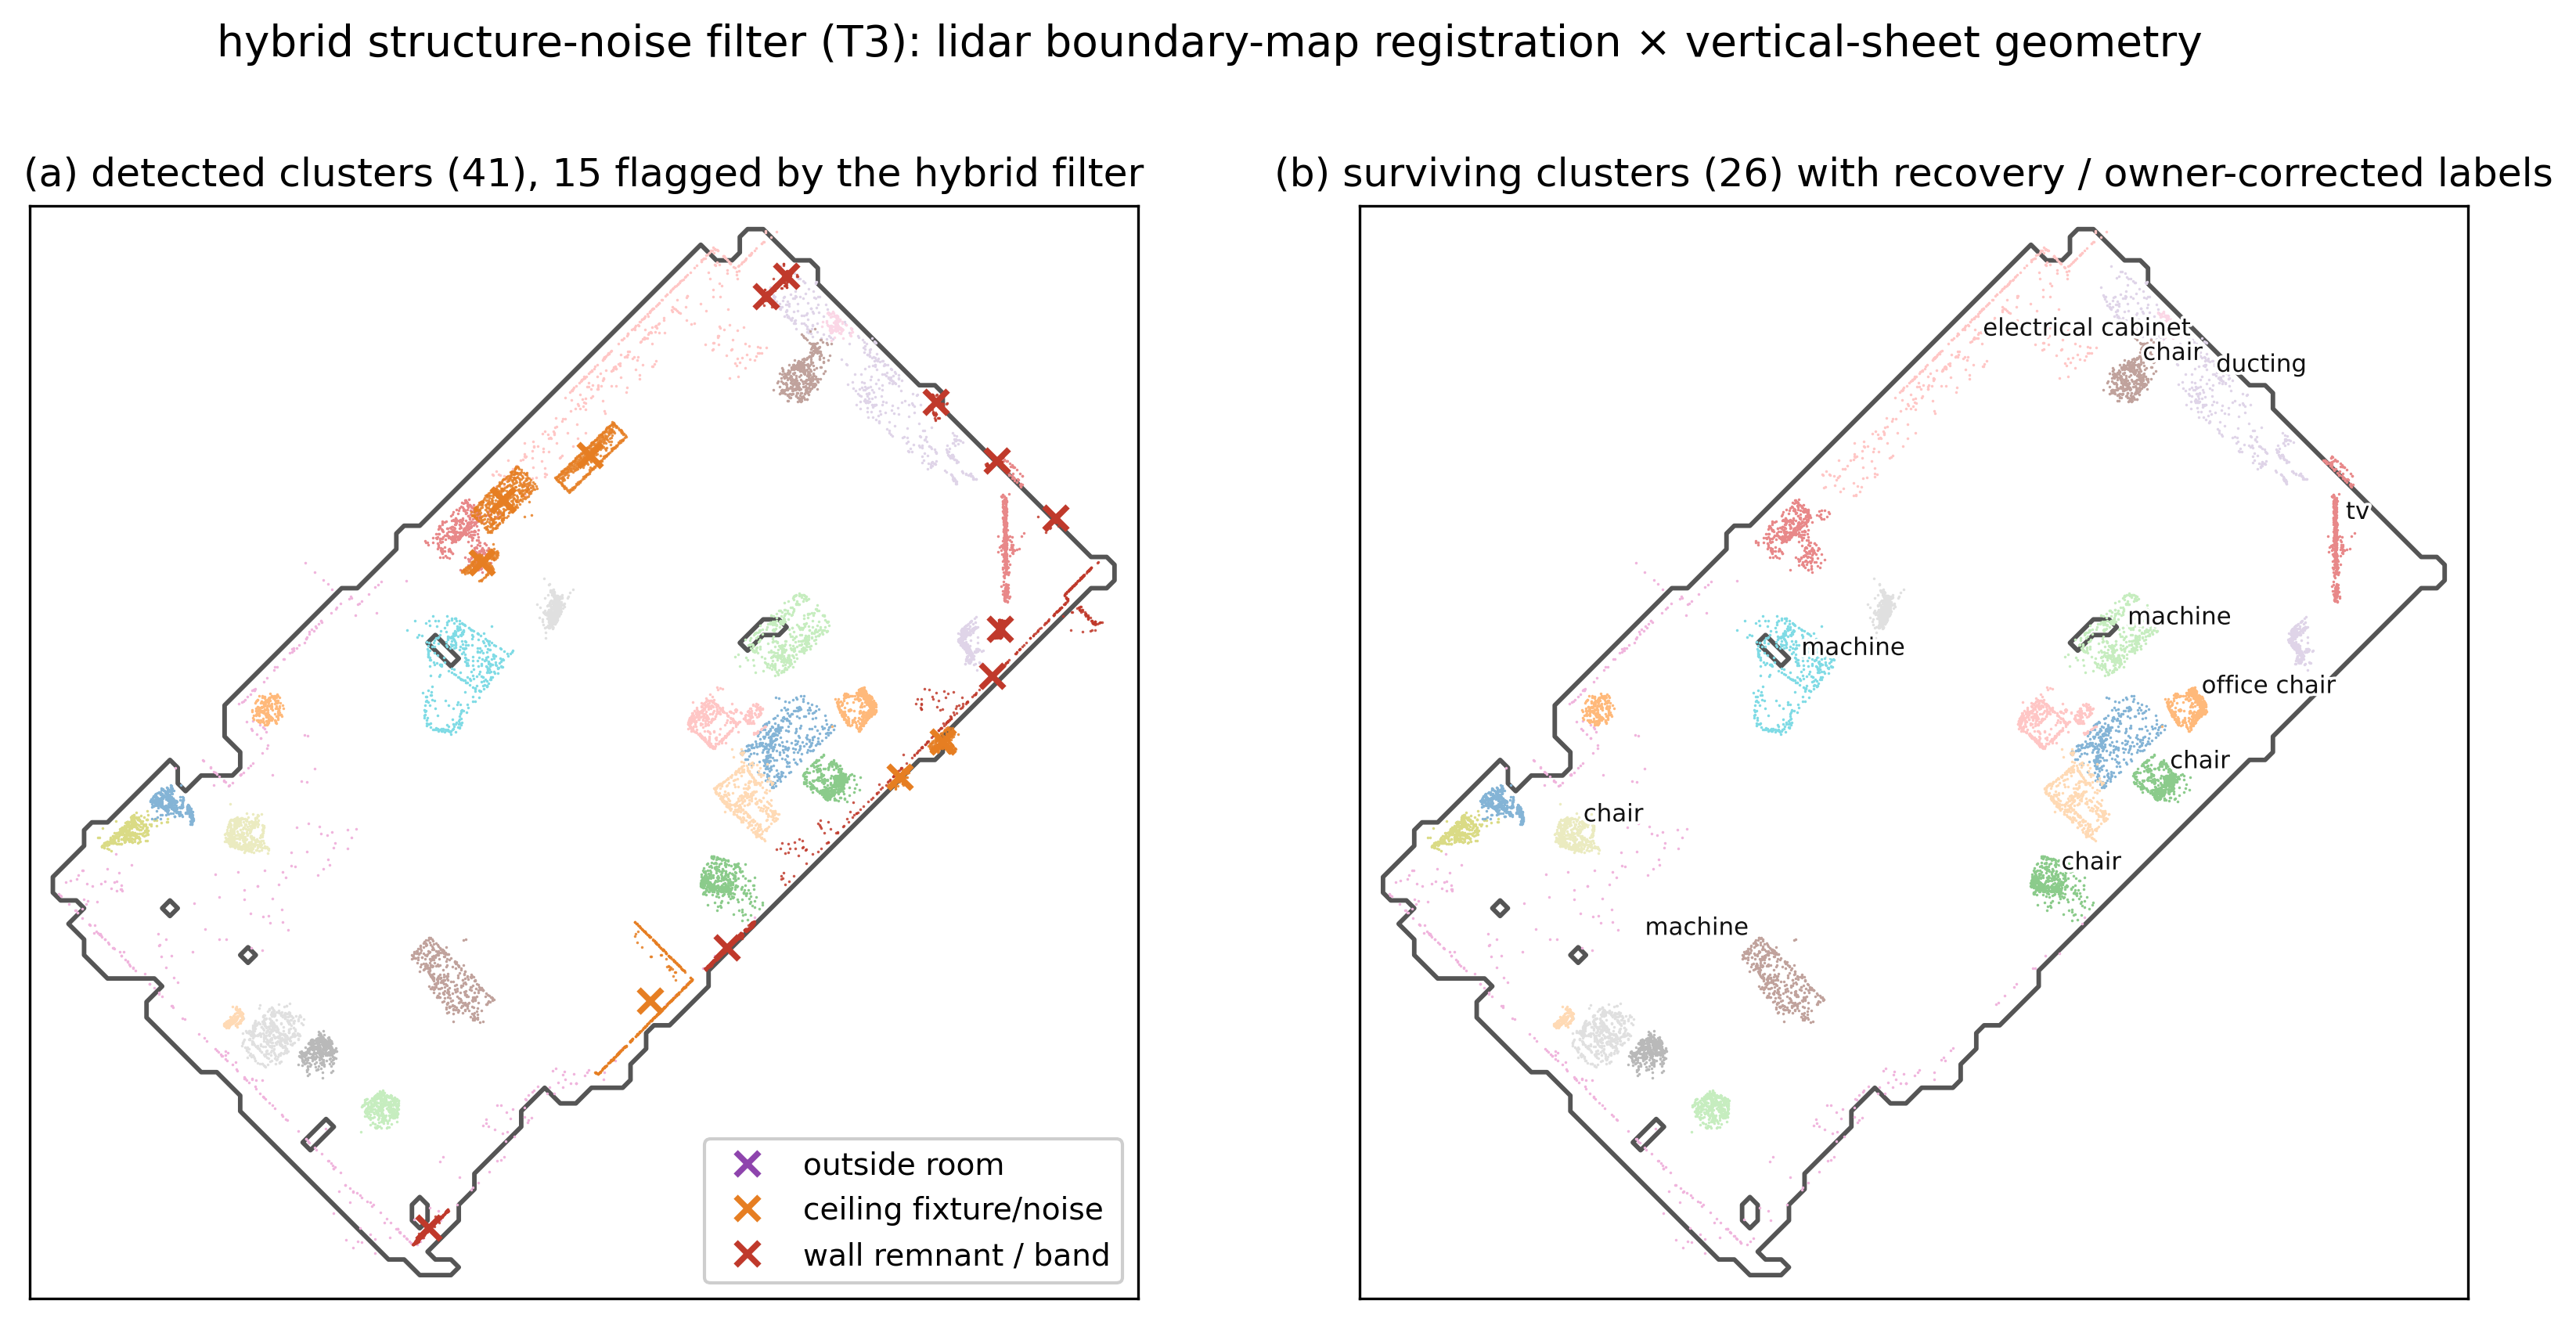
\includegraphics[width=\linewidth]{fig14_structure_filter.png}
\caption{Hybrid structure-noise filter on the T3 epoch. (a) All 41
detected clusters; the 15 flagged ones are colored by rule --- wall
remnant/band (grid-map hug $\times$ thin vertical sheet, or long
full-height band), ceiling fixture/noise, outside the room boundary.
(b) The 26 survivors with recovery / owner-corrected labels. The
wall-flush monitor bank (labeled \texttt{tv}) and wall-mounted equipment
survive; residual merge labels (\texttt{electrical cabinet},
\texttt{ducting}) are retained pipeline output, not corrections.}
\label{fig:structfilter}
\end{figure}

\begin{figure}[t]
\centering
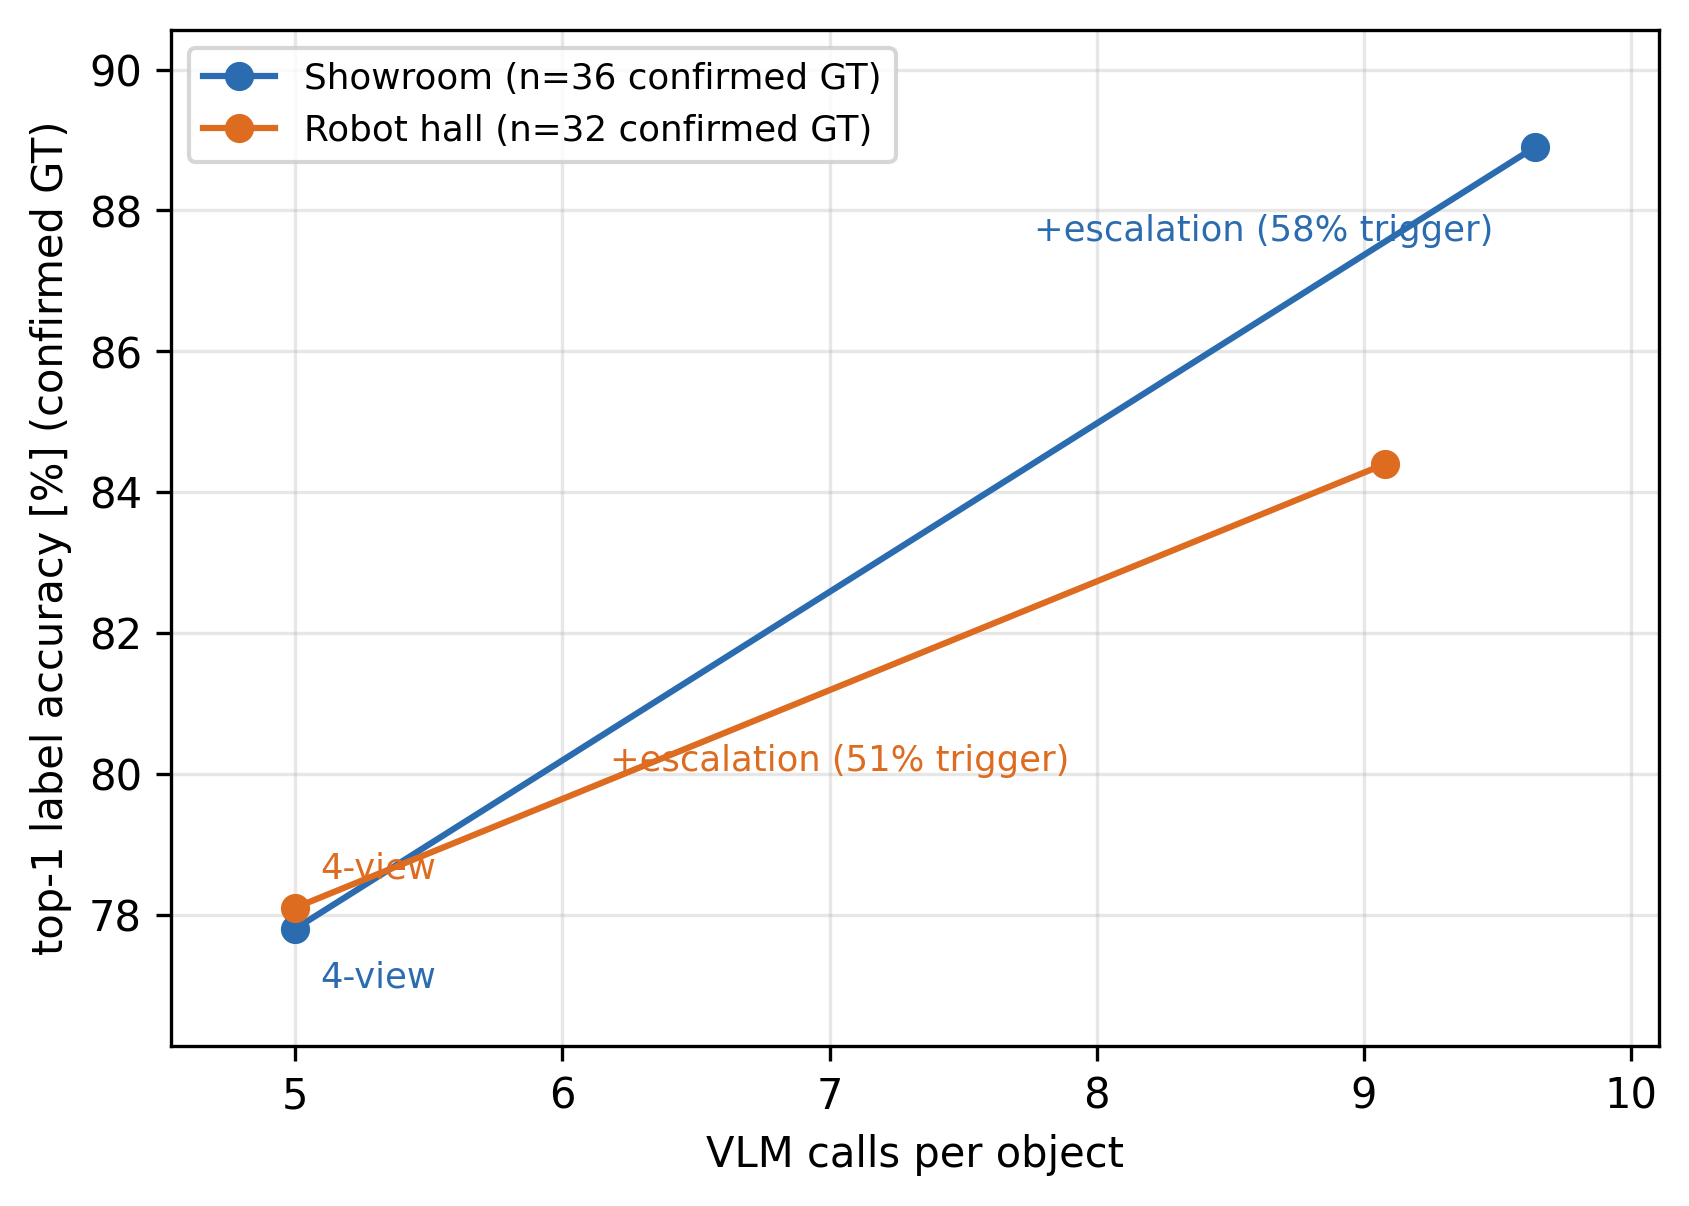
\includegraphics[width=0.85\linewidth]{fig6_escalation_cost.png}
\caption{Escalation accuracy--cost curves for both scenes.}
\label{fig:esccost}
\end{figure}

\begin{figure}[t]
\centering
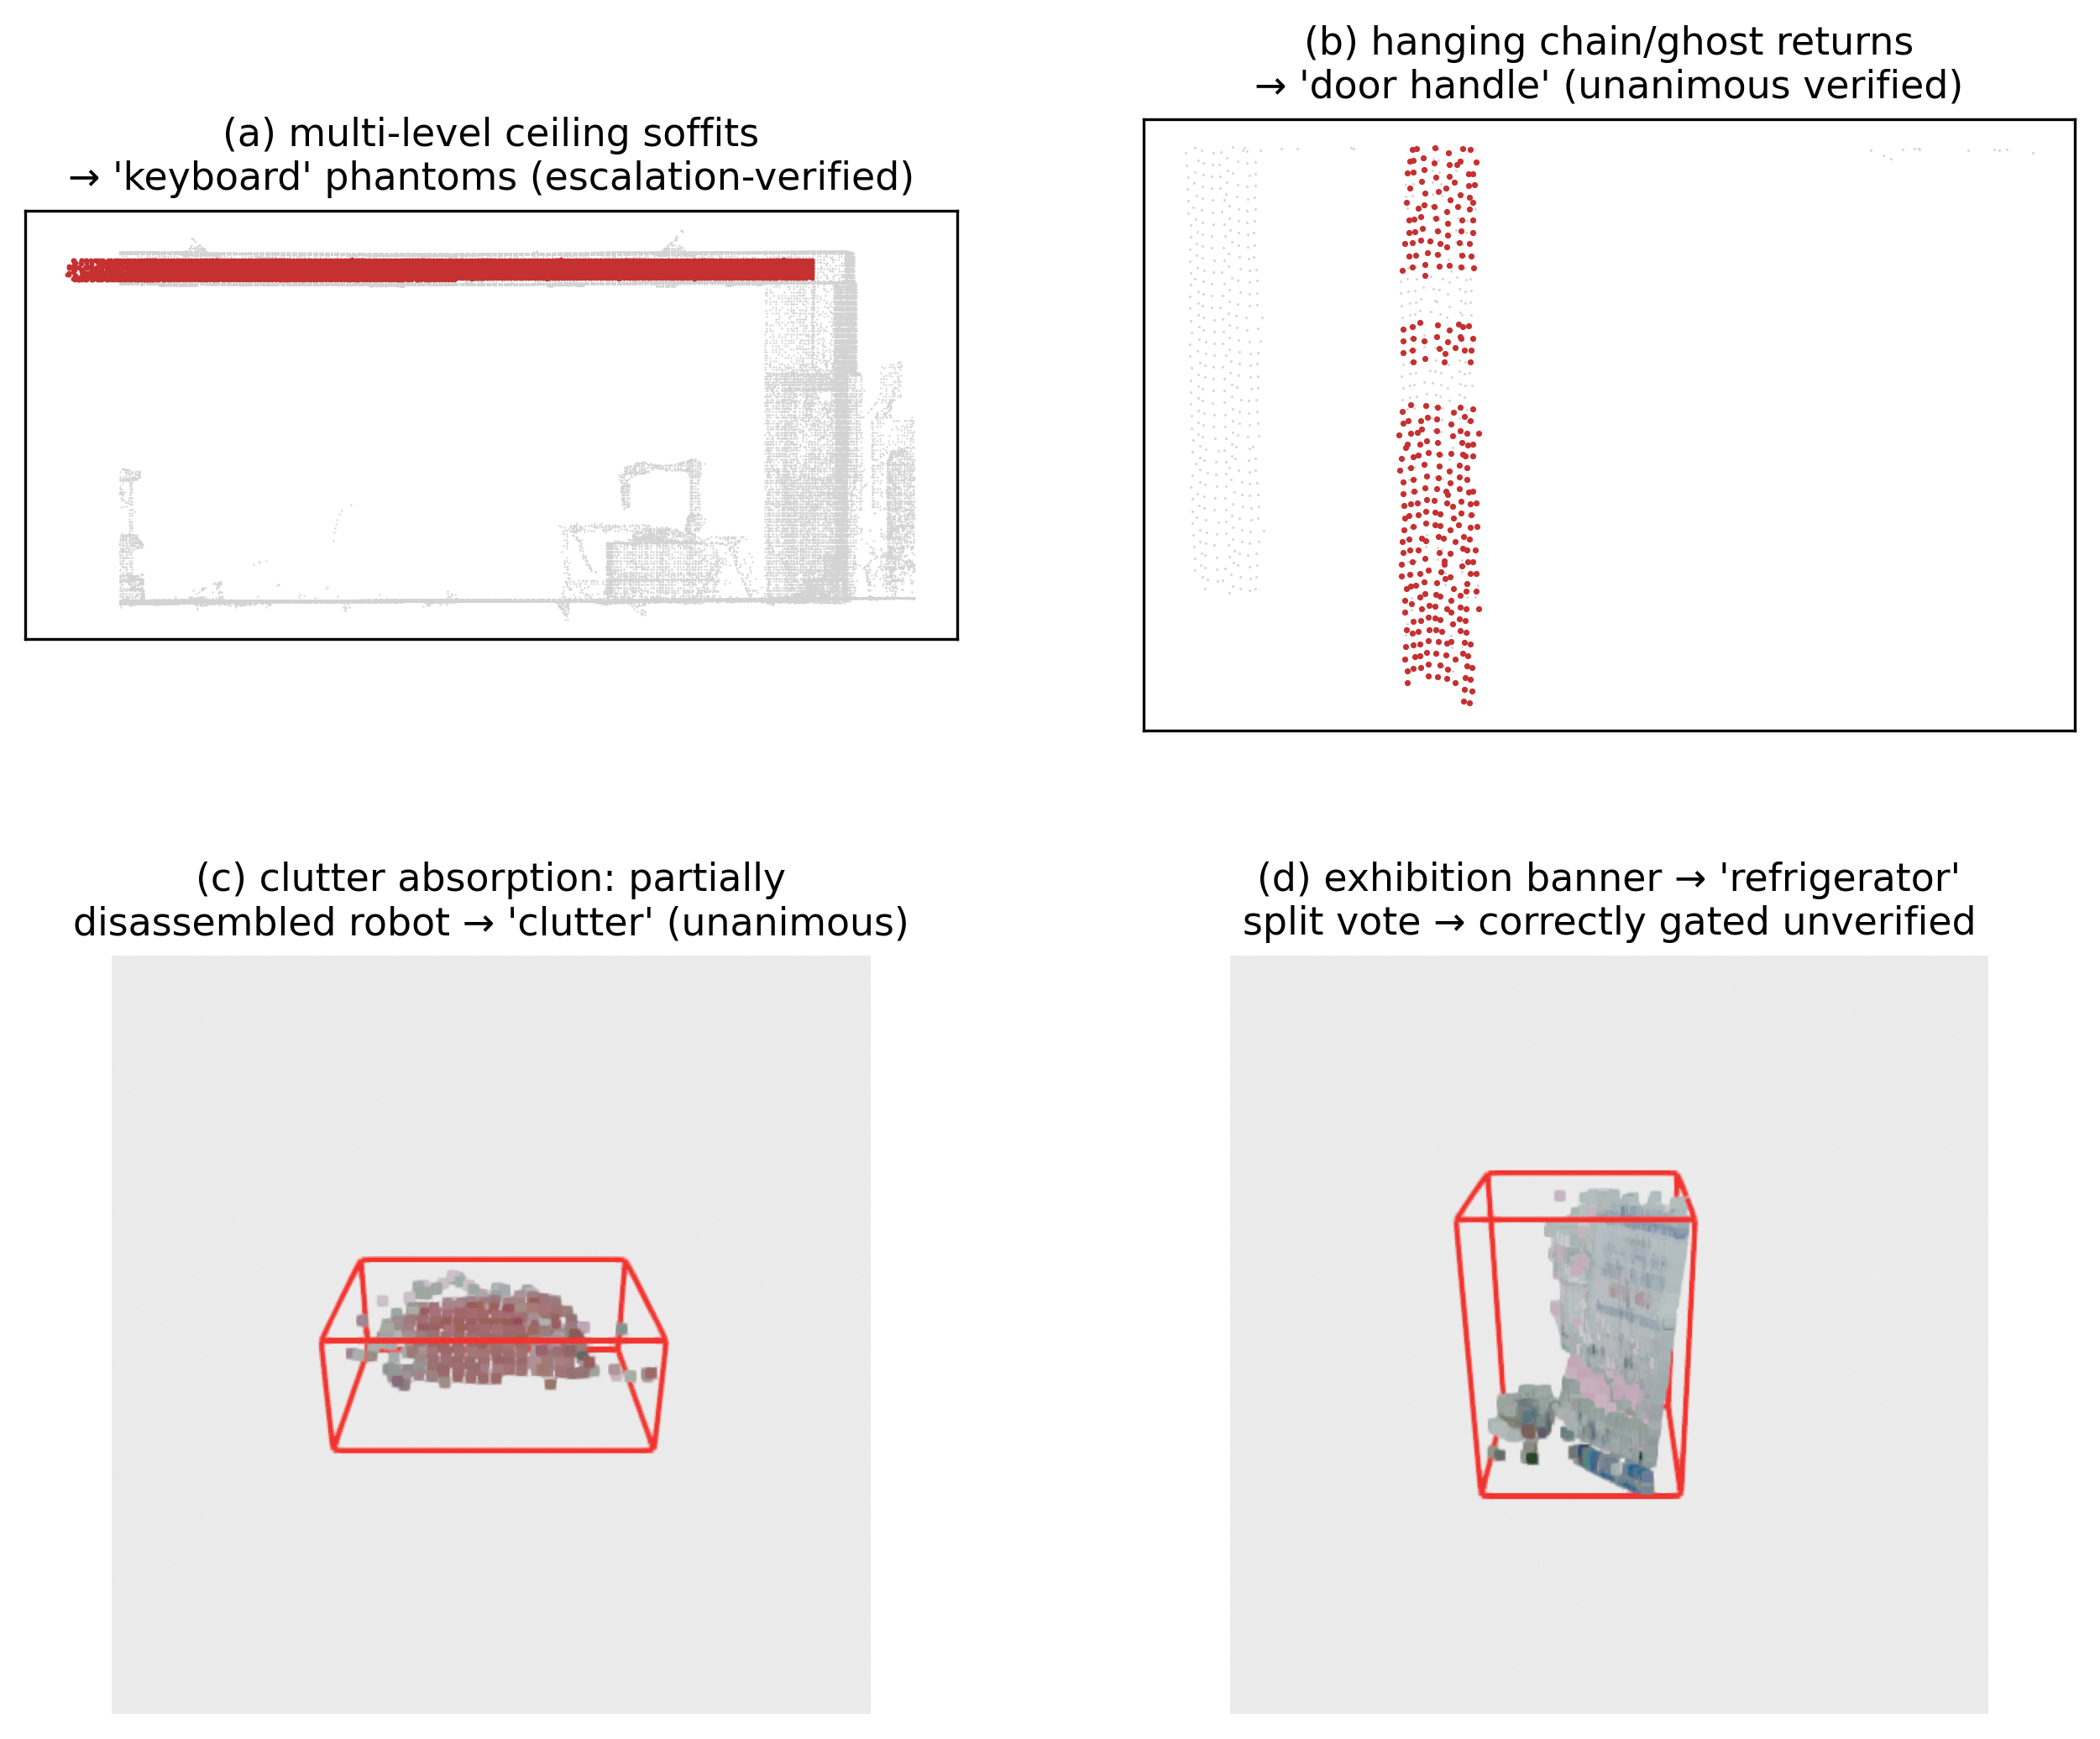
\includegraphics[width=0.9\linewidth]{fig10_error_taxonomy.png}
\caption{Verification error taxonomy: remnant phantom, unanimous-but-wrong,
clutter absorption, render ambiguity.}
\label{fig:taxonomy}
\end{figure}

\subsection{Knowledge-Grounded Query Evaluation}
\label{sec:exp-query}

We evaluate four conditions over identically constructed per-scene query
sets---48 items on the showroom, 32 on the robot hall (symbolic, explicit,
scene-level, and trap questions): (1) \emph{LLM-only} (Stage-A dump, no
verification), (2) \emph{ungated KG}, (3) \emph{verified-only KG}
(unverified nodes removed), and (4) \emph{gated KG} (unverified retained but
structurally demoted, Sec.~\ref{sec:query}). Each scene carries four trap
questions about objects that do not exist as labeled. On the showroom all
four traps target \emph{unverified-label} phantoms (keyboard, ladder); on
the robot hall two target an unverified-label phantom (refrigerator) and
two an \emph{escalation-verified} phantom (keyboard)---the latter probing
the gate's verifier-quality bound. A correct system must decline to assert
the trap labels. Note that LLM-only can ``block'' traps trivially: with no
map it tends to deny that specific objects exist at all (4/4 on the robot
hall, 2/4 on the showroom), so trap blocking is diagnostic only for the
grounded conditions.

\begin{table}[t]
\centering
\caption{Query benchmark, four conditions (accuracy / hallucination rate /
traps blocked), with abstention counts. Question sets: showroom $n{=}48$
(14 symbolic, 12 explicit, 9 implicit, 9 scene-level, 4 trap); robot hall
$n{=}32$ (15 symbolic, 12 explicit, 1 scene-level, 4 trap). An abstention
counts against accuracy (the denominator is always $n$) but is not a
hallucination; the verified-only condition's low accuracy is largely its
abstention cost.}
\label{tab:query}
\footnotesize
\setlength{\tabcolsep}{3pt}
\begin{tabular}{@{}lcccc@{}}
\toprule
 & LLM-only & Ungated & Verified-only & Gated \\
\midrule
Showroom ($n{=}48$) & 52.1\% / 20.8\% / 2/4 & 81.2\% / 18.8\% / 0/4 &
58.3\% / 16.7\% / 4/4 & \textbf{83.3\% / 16.7\% / 3/4} \\
\quad abstentions & 13 & 0 & 12 & 0 \\
Robot hall ($n{=}32$) & 50.0\% / 37.5\% / 4/4 & 56.2\% / 43.8\% / 0/4 &
46.9\% / 40.6\% / 2/4 & \textbf{59.4\% / 40.6\% / 2/4} \\
\quad abstentions & 4 & 0 & 4 & 0 \\
\bottomrule
\end{tabular}
\end{table}

On the showroom (Table~\ref{tab:query}, Fig.~\ref{fig:query}), grounding
alone (ungated) lifts
accuracy from 52.1\% to 81.2\% but blocks no traps; removing unverified
content (verified-only) blocks all four traps at a steep recall price (12
abstentions, 58.3\%); the gated condition is the balance point---83.3\% with
3/4 traps blocked. The two leaks are instructive and mechanistically
distinct. On the showroom, one \emph{count}-phrased trap slipped through
the quarantine itself: the model tallied a demoted node by reading its
\texttt{failedCandidateType} field, even though it correctly denied the
same object in yes/no phrasing. On the robot hall, the keyboard phantom is
\emph{escalation-verified}, so it passes any status-based gate---gating is
bounded by verifier quality; we report both as properties, not anomalies.
The robot hall reproduces the ordering at lower absolute levels because its
end-to-end label errors (banner$\rightarrow$refrigerator,
robot$\rightarrow$clutter) propagate into every grounded condition---an
honest end-to-end number rather than a curated one. We note the statistical
scope explicitly: at $n{=}48$/$32$ questions the gated-vs-ungated
\emph{accuracy} gap is a single question on each scene, so the benchmark is
diagnostic rather than powered for significance. The case for gating rests
on the mechanisms the benchmark isolates---trap blocking, the abstention
structure, and the direction of the hallucination change---and on the
downstream mission-level consequences of Sec.~\ref{sec:semnav}, not on the
accuracy deltas alone.

\begin{figure}[t]
\centering
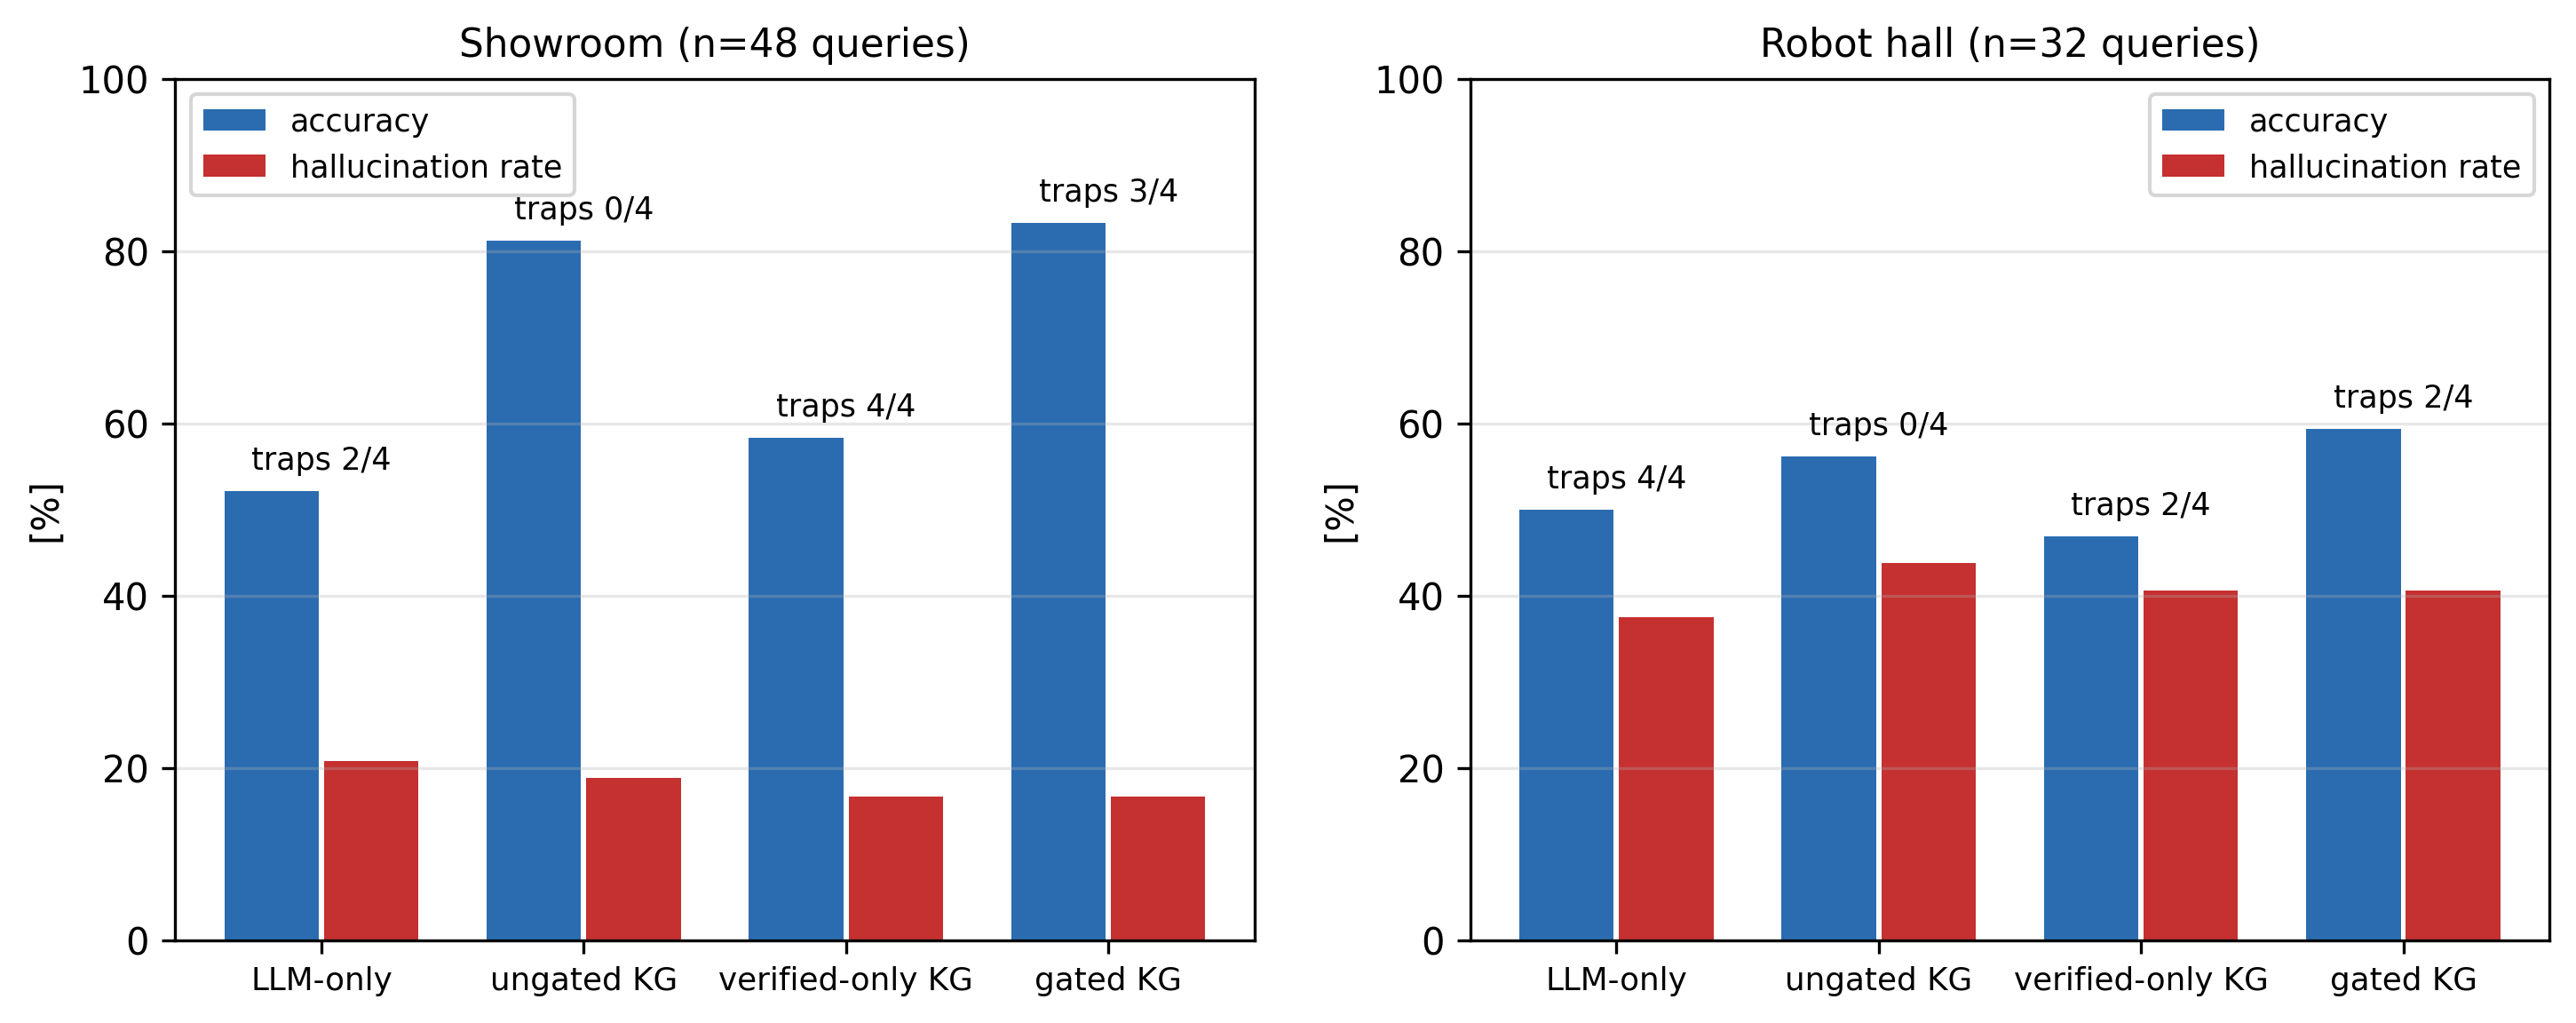
\includegraphics[width=0.9\linewidth]{fig7_query_benchmark.png}
\caption{Four-condition query benchmark with trap-question panel.}
\label{fig:query}
\end{figure}

\subsection{Incremental Update Evaluation}
\label{sec:exp-update}

\paragraph{Synthetic scenarios.}
Controlled edits of the room-scoped robot hall isolate matcher behavior
(Fig.~\ref{fig:update}): \emph{(A) unchanged repeat}: 55/55 nodes carried,
zero VLM calls, zero identity switches; \emph{(B) move}: 1/1 moved with ID
preserved; \emph{(C) remove+insert}: exact absent/insert classification;
\emph{(D) occlusion}: at 20\% crop both affected objects still match (as
updated, labels kept), at 40\% matching fails into 2 false-absents + 2
false-news---the matcher's quantified breaking point, and the motivation for
overlap-based matching features in future work. On the combined-edit
re-scan (move, insertion, and removal applied together), selective
re-verification re-ran Stage B on only the two changed clusters: 26 of 822
VLM calls, \$0.23 versus \$7.37 for a full re-verification---3.1\% of
rebuild cost, and 0\% for scenario A. We scope this claim precisely: the
3.1\% figure comes from this controlled same-quality re-scan, where
unchanged clusters reproduce byte-identically. On the real
T2$\rightarrow$T3 transition the scan protocol itself changed
(higher-coverage acquisition), no cluster hash matched, and the epoch paid
full verification cost (\$3.54 for 41 clusters)---zero-cost carry-over is
a property of reproducible acquisition, not of the update mechanism alone.

\paragraph{Real three-epoch study.}
The three epochs of Table~\ref{tab:scenes} form a real update sequence:
T1 (manual, June) $\rightarrow$ T2 (exploration, early July) $\rightarrow$
T3 (99.6\%-coverage exploration with a controlled-change protocol, late
July). Cross-epoch registration is fully automatic
(FPFH~\cite{rusu2009fpfh}+RANSAC then ICP~\cite{besl1992icp};
5.1\,cm RMSE for T1$\rightarrow$T2, 4.2\,cm for T3$\rightarrow$T2). The
T1$\rightarrow$T2 diff records the room's exhibition-to-test-hall
reorganization (updated 4 / moved 3 / inserted 48 / absent 31; among the
moves, a fire extinguisher displaced 3.0\,m). This epoch also motivated the
generic-type exclusion in the move pass: without it, clutter piles matched
across 2--5\,m as fictitious ``moves'' (9 candidates, 3 credible).
The T2$\rightarrow$T3 diff (matched 9 / moved 1 / inserted 31 / absent 45,
Fig.~\ref{fig:epochs}) sits on top of measured natural drift: only 65\% of
in-room object geometry is mutually supported at 10\,cm between the two
scans two weeks apart---roughly a third of the room changed before any
protocol was applied.

\emph{Matching scorecard.} To score the real transitions without circular
reference to the matcher itself, we built an independent correspondence
reference by bidirectional point overlap between epochs (5\,cm
association, both directions $\ge$0.5 for a strong pair, 0.3--0.5
partial; the same construction as the T1 GT transfer of
Sec.~\ref{sec:exp-verify}), and replayed the recorded upserts against it.
The reference finds 4 strong and 6 partial static pairs for
T1$\rightarrow$T2 and 7 strong and 5 partial for T2$\rightarrow$T3.
Matching accuracy on strong pairs is 2/4 and 4/7; \textbf{identity
switches are zero on both transitions}---every miss is a
\emph{fragmentation} error in which re-segmentation changed an extent
beyond the 30\% tolerance, so the object was marked absent and
re-inserted under a new ID, never associated to the wrong object. The
per-miss diagnosis is uniform: all five failed the per-axis extent gate
(the most consequential case is the T3 ``new'' fire extinguisher, whose
cluster overlaps a T2 \texttt{clutter} cluster at 0.96--0.99 mutual
overlap but with width 0.11 vs.\ 0.28\,m). Strict false-new and
false-absent counts are 2/2 (T1$\rightarrow$T2) and 3/3
(T2$\rightarrow$T3), rising to 5/5 and 3/3 if partial pairs are also
demanded; nine split/merge cases (one cluster absorbing several) are
reported separately rather than forced into either bin. Multi-candidate
conflicts---the greedy resolution of Sec.~\ref{sec:matching}---occurred
zero times in pass~1 on both transitions and once in pass~2, where
nearest-centroid arbitration picked the owner-confirmed 0.64\,m chair
move. All three recorded \texttt{moved} claims are consistent with the
reference (a true move has no in-place overlap, so the reference can
refute but not confirm identity; the chair move is additionally
owner-confirmed). Repeating the reference construction at 10\,cm
association (twice the registration RMSE) leaves identity switches at
zero.

Against the controlled-change protocol, the system detected \textbf{2/2
physical changes at geometry level}: the moved chair is the epoch's
\emph{only} \texttt{moved} node (0.64\,m, ID preserved---a node matched
continuously since T1), and the introduced floor fan was correctly
\texttt{inserted} but typed \texttt{clutter} (error class (c) above), giving
1/2 at type level. Identity persistence is demonstrated across all three
epochs: the fire extinguisher, pump, industrial robot, and several chairs
retain their minted IDs through both reorganizations. The live graph has
since accumulated thirteen revisions through the same mechanism ---
rescans, owner refutations/restorations/corrections, re-split
decompositions, and finally a stale-node sweep in which eighteen
earlier-epoch detections with no support in the current scan were marked
absent; every transition, including the mistakes it corrects, is
reconstructible from node histories. The place layer
re-derives per-epoch names on the same SLIC regions
(Sec.~\ref{sec:place}): exhibition-era \texttt{machine\_access\_area} and
\texttt{operator\_control\_station} become clutter-dominated at T2 and
\texttt{machine\_operator\_station}/\allowbreak
\texttt{electrical\_services\_zone} at T3, at $\sim$\$0.03 per epoch.

\begin{figure}[t]
\centering
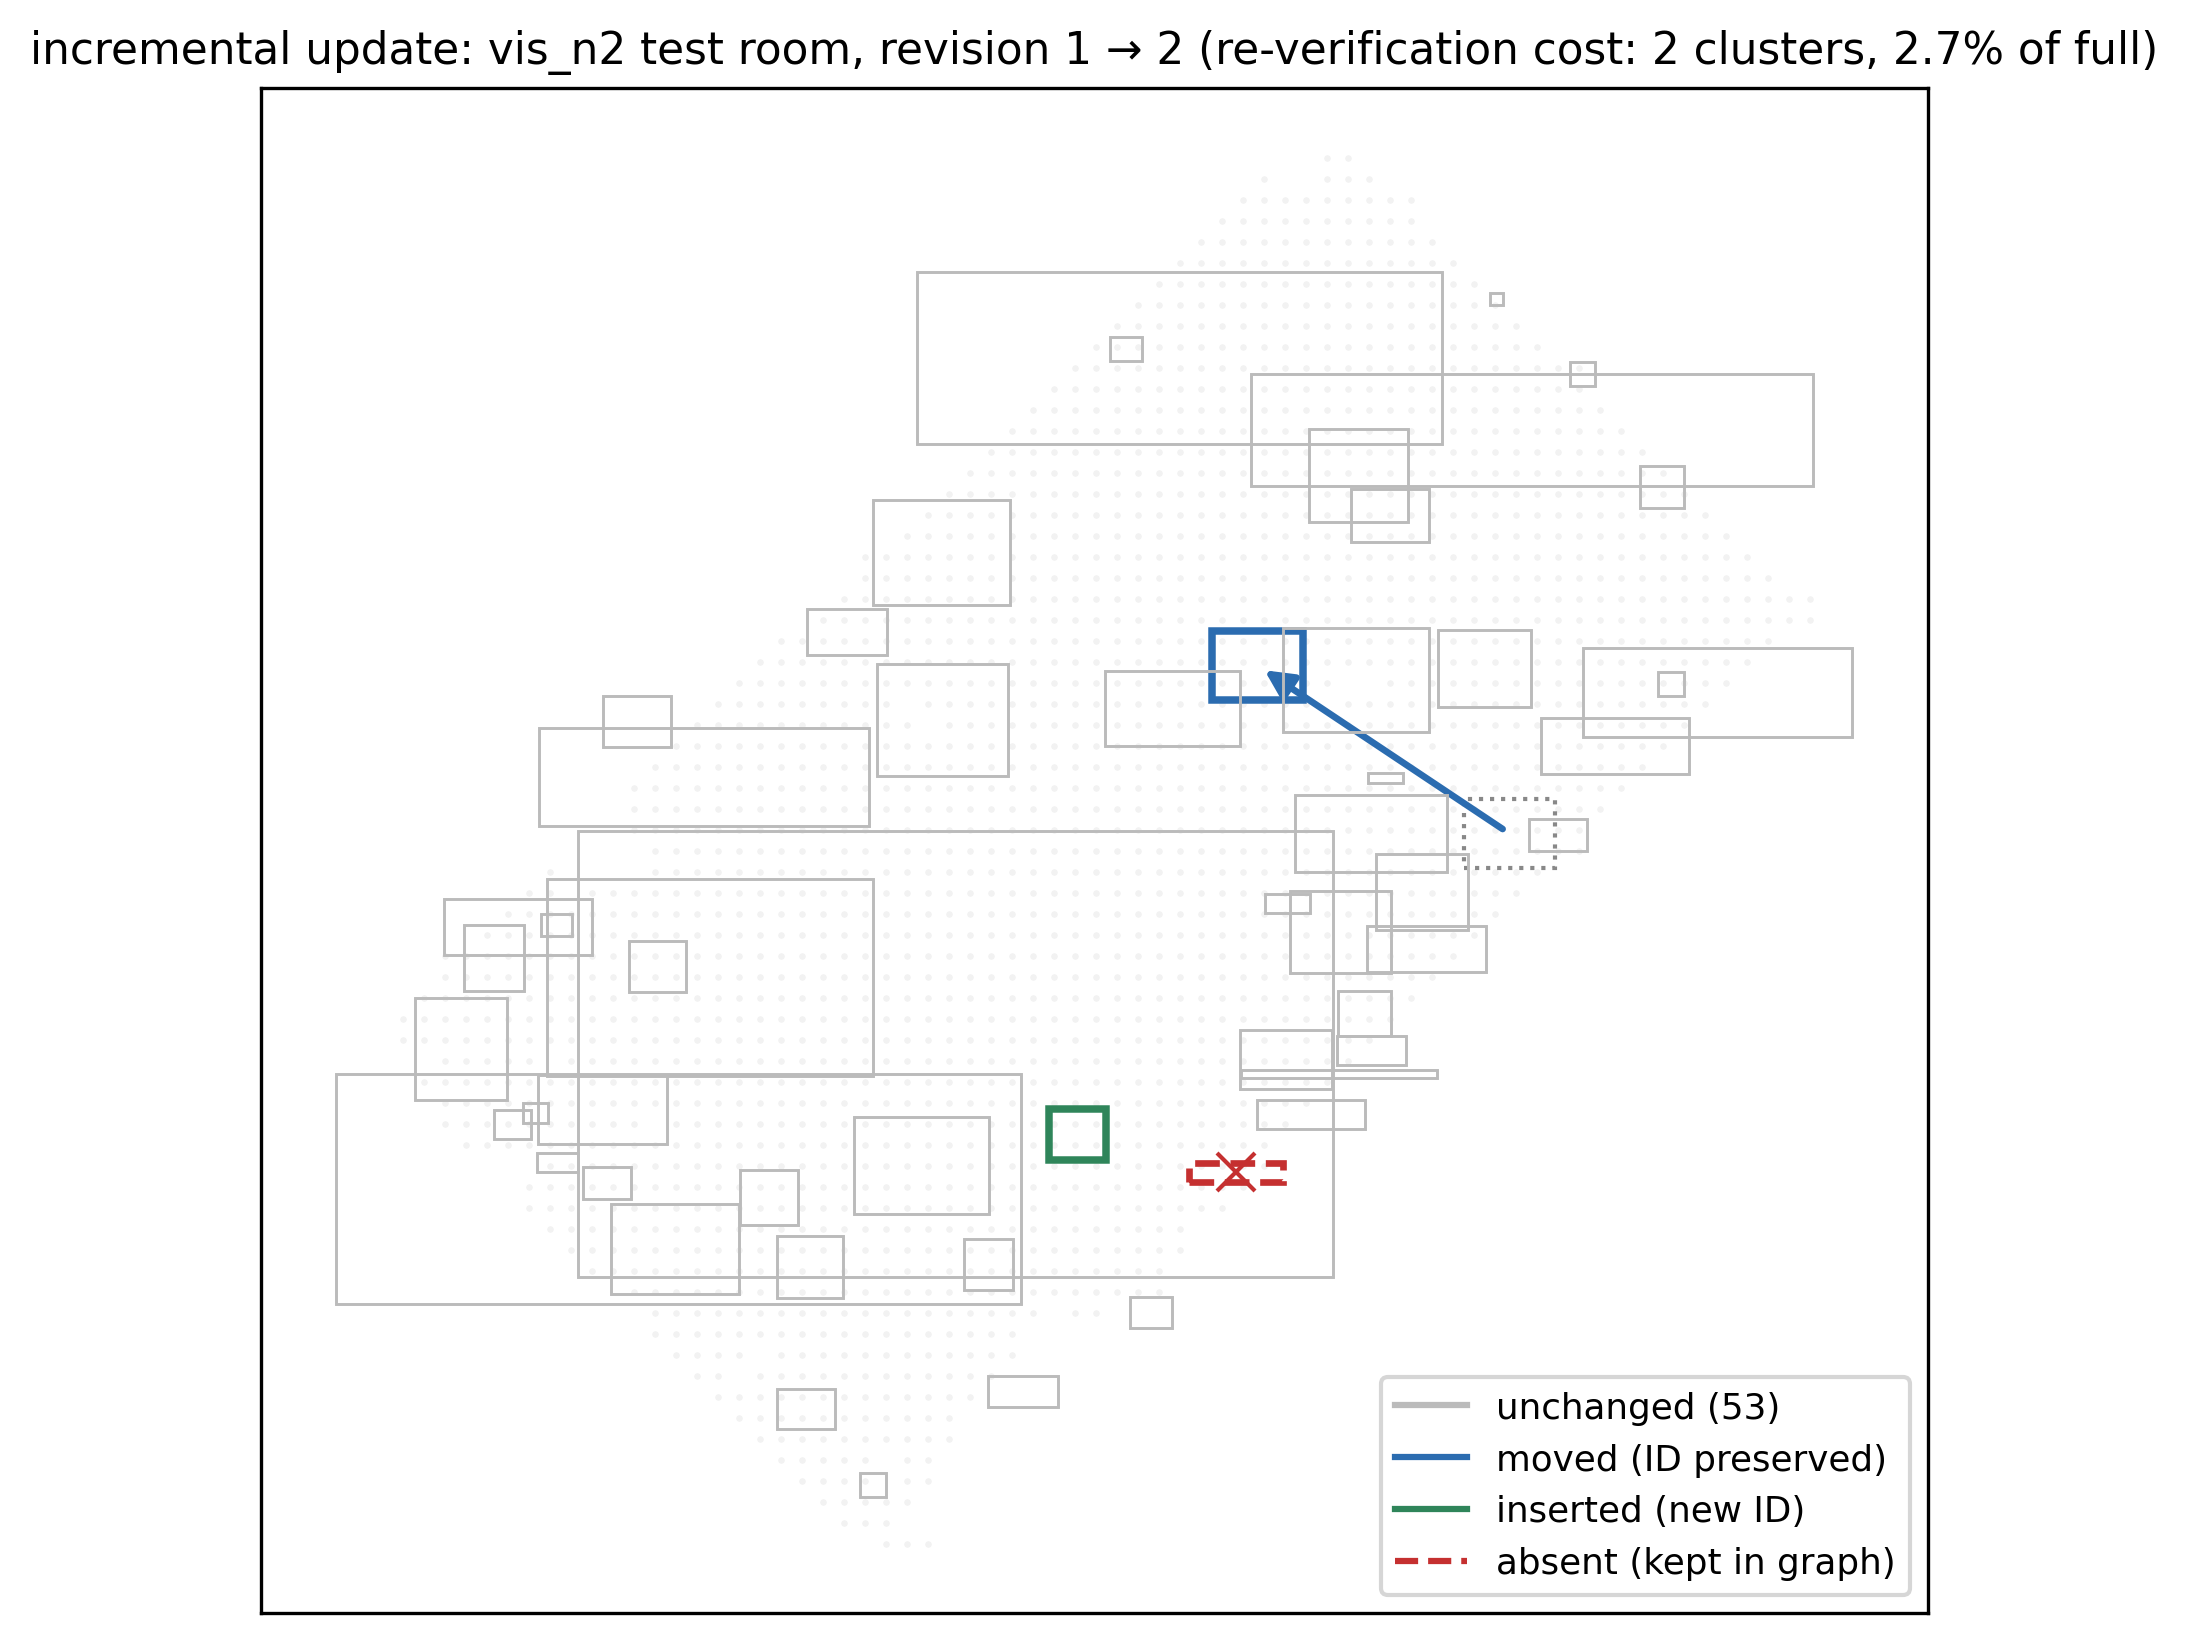
\includegraphics[width=0.9\linewidth]{fig8_incremental_update.png}
\caption{Controlled re-scan scenarios A--D (room-scoped robot hall, 55
objects), top-down view. Colored points are the segmented clusters, thin
rotated rectangles their explicit-model footprints with node names, and the
dark contour the test-room boundary; each edited object is annotated with
the matcher's decision. (A)~A repeat scan with no changes
carries all 55 verdicts at zero VLM cost. (B)~A 3.6\,m chair move is
classified \texttt{moved} with its node ID preserved. (C)~A removed object
is marked \texttt{absent} (node kept and flagged) and a newly placed object
is \texttt{inserted} under a new ID; only the insertion is re-verified. (D)~Partial occlusion: both cropped objects still match at 20\%,
but at 40\% matching fails into two false-absent plus two false-new
pairs---the matcher's quantified breaking point.}
\label{fig:update}
\end{figure}

\begin{figure}[t]
\centering
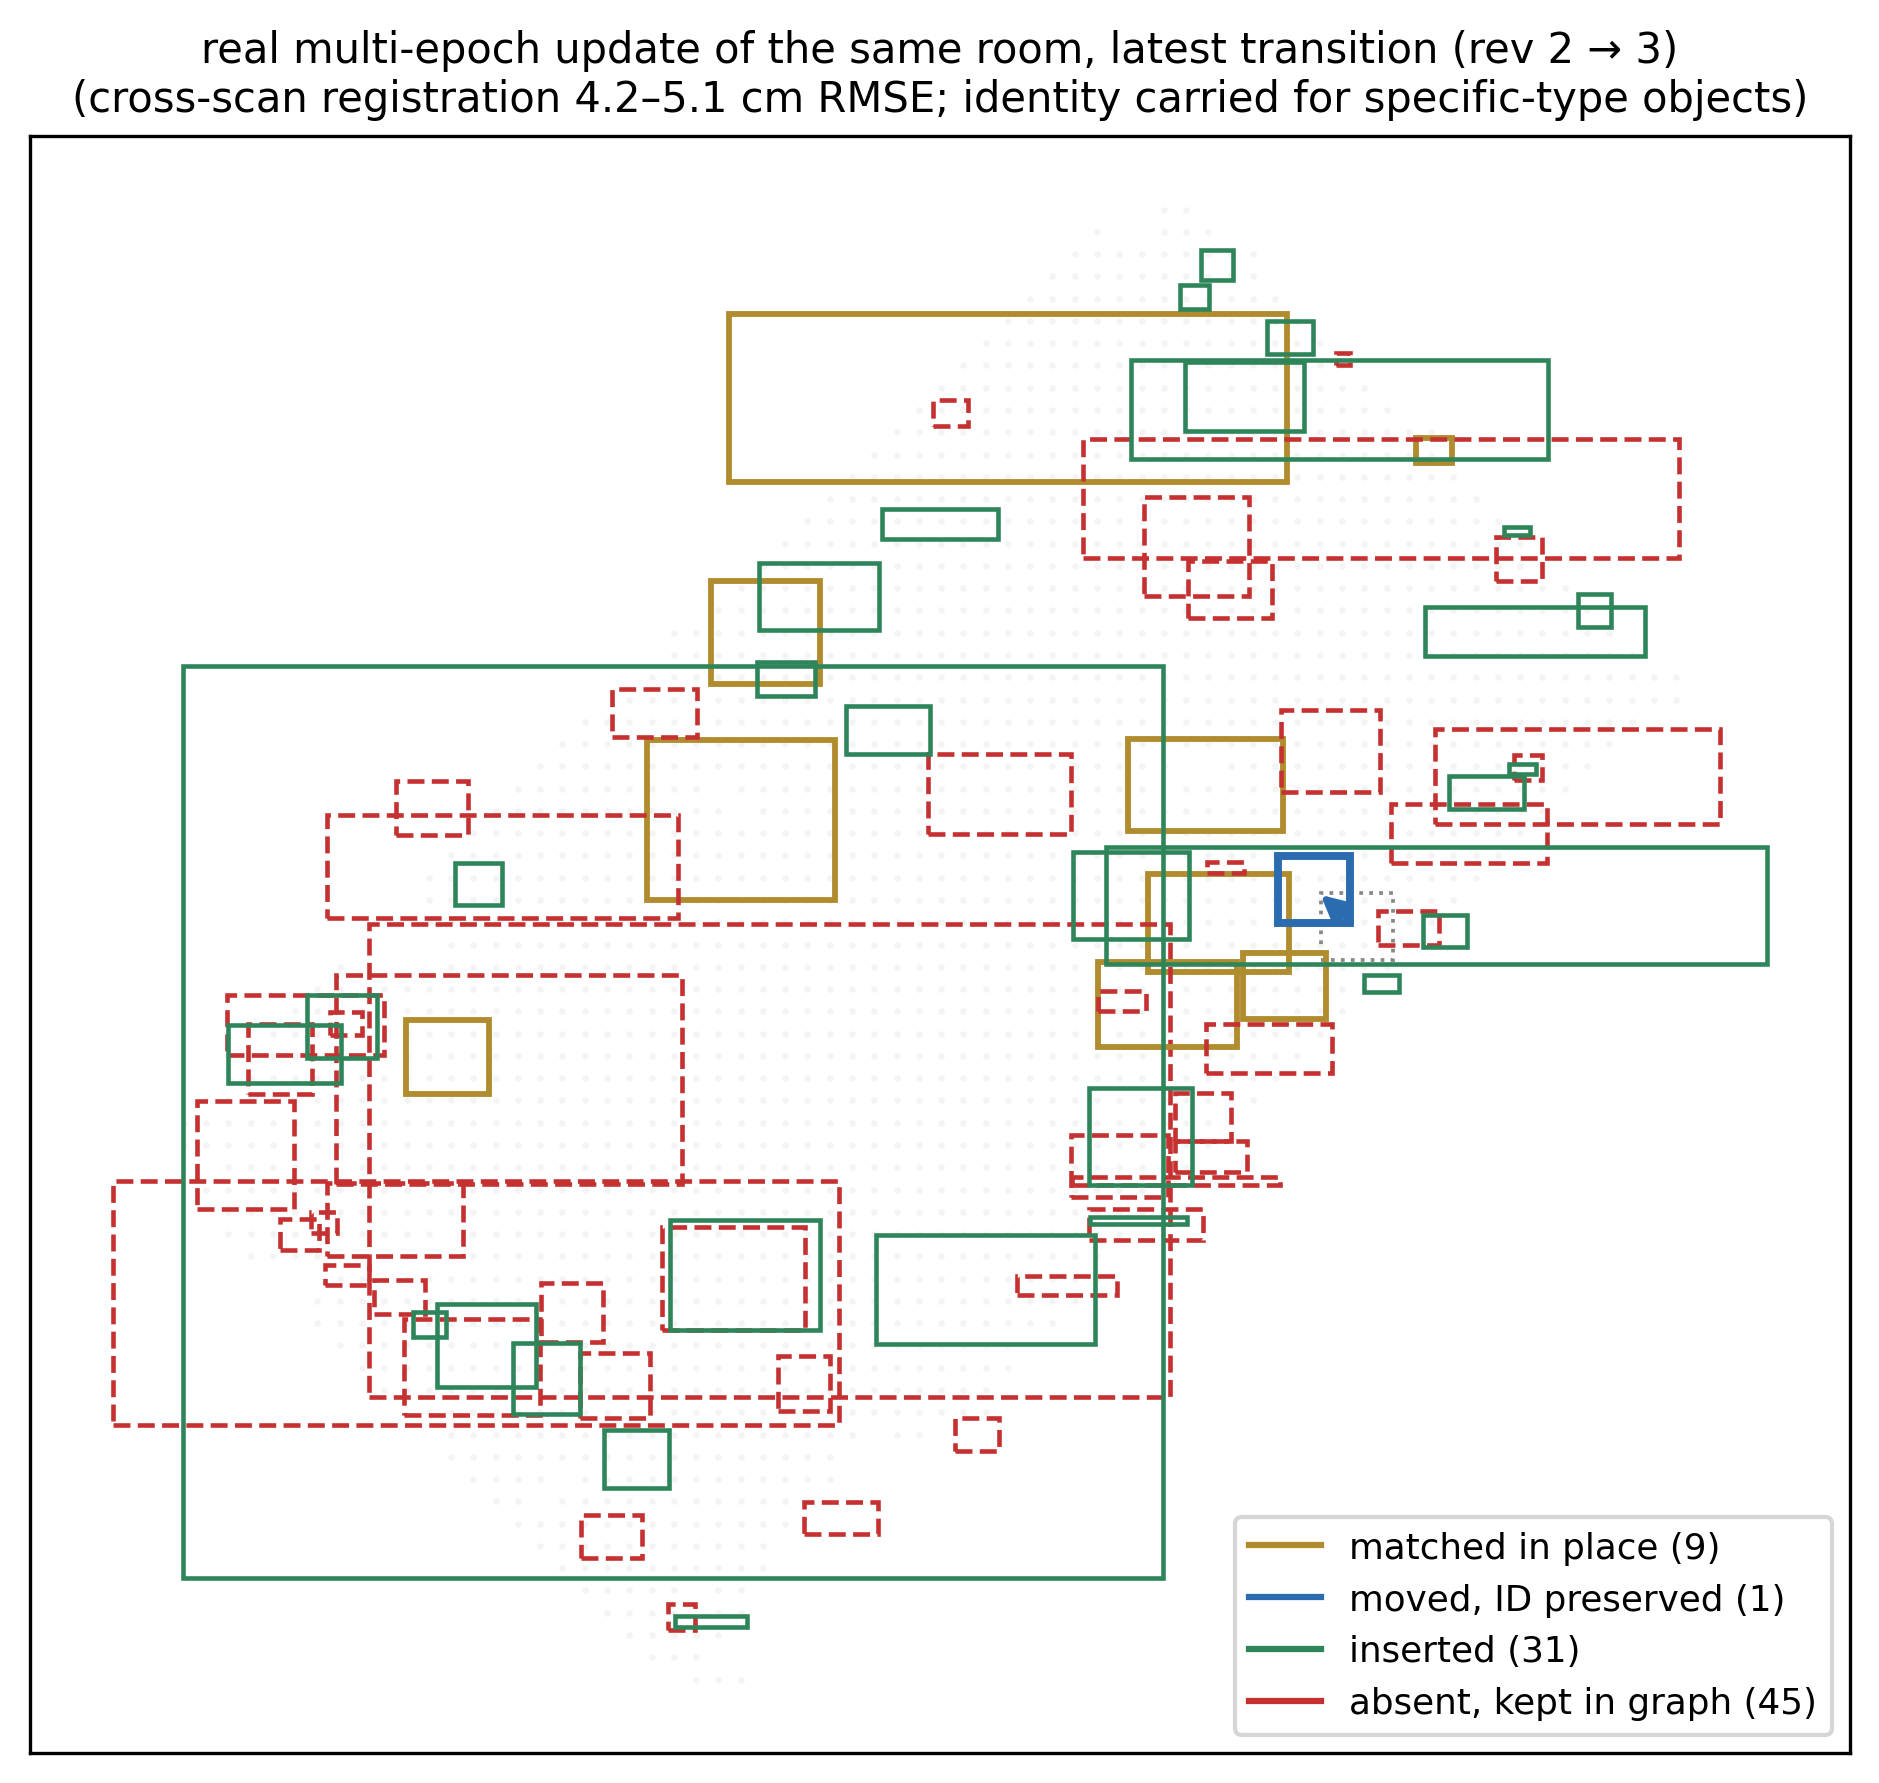
\includegraphics[width=0.9\linewidth]{fig9_two_epoch_update.png}
\caption{Real multi-epoch update, latest transition (T2$\rightarrow$T3),
top-down view. Colored points are the T3 segmented clusters inside the
test-room boundary; yaw-rotated node footprints are colored by diff state
(matched, moved with ID preserved, inserted, absent), with names on
specific-type objects. Oversized footprints of merged mega-clusters
(e.g., \texttt{machine\_012}, Sec.~\ref{sec:exp-ablation}) are faded.}
\label{fig:epochs}
\end{figure}

\subsection{Retrospective End-to-End Replay against Accumulated Owner
Ground Truth}
\label{sec:exp-endtoend}

After the corrective machinery of Secs.~\ref{sec:exp-seg}--\ref{sec:exp-update}
stabilized, we re-ran the entire pipeline from the raw scan with no owner
input at execution time and scored it against the live knowledge graph ---
by then a 46-object inventory embodying every owner restoration,
refutation, and correction. Because the corrective mechanisms were
developed from failures observed in this same environment, this
experiment is a \emph{retrospective end-to-end replay} on the
development scene, not an independent generalization test; what it
measures is how much of the owner-audited inventory the automated
layers recover once owner-informed development has concluded. The
replay runs the \emph{frozen} pipeline exactly as defined in
Secs.~\ref{sec:preprocess}--\ref{sec:corrective}---every trigger and
threshold fixed, no per-scene adjustment, no owner input at execution
time---so it is an independent \emph{run}, on a non-independent
\emph{scene}. The cafeteria (Sec.~\ref{sec:exp-ablation}) is the only
scene that is independent in both senses, and a multi-building
evaluation remains future work
(Sec.~\ref{sec:discussion}). One
corrective layer transfers mechanically and can therefore be checked
held-out: applying the hybrid structure filter to the cafeteria with
its T3 rules frozen (the occupancy-grid prior synthesized from the
scan's floor points) flags both ceiling-noise clusters with zero false
positives---both wall-flush doors survive, the trade-off that cost a
poster stand on T3---while the wall pillar evades the wall-hug test
and the seven carpet floor-noise clusters fall outside its rule
families entirely, consistent with the floor-material gap of
Sec.~\ref{sec:discussion}. The remaining corrective layers embed
scene-specific owner evidence by construction and are not claimed to
transfer. Table~\ref{tab:layers} reports cumulative geometric recall as
each automated layer is enabled. The verified path alone recovers 28\%;
diffuseness-gated re-splitting nearly doubles it; the wall-compound gate
(which self-triggers on the monitor wall and decomposes it into nine of
the ten owner-confirmed units) and the structure-condition ensemble bring
automated recall to 85\%. Type accuracy saturates far lower
($\sim$31\% of recalled objects) --- the label bottleneck is the
correlated verifier bias of Sec.~\ref{sec:exp-seg}, and closing it is
precisely the owner layer's role. For calibration within the lineage's
own reporting style, DK-SMF reports 78--81\% detection accuracy against
predefined ground-truth objects in its RGB-D environments~\cite{joo2025dksmf};
our 85\% is measured against an owner-audited inventory that includes
partially scanned and wall-flush objects, though the sensing modality
and ground-truth protocols differ. The re-run also reproduced the
deterministic backbone's stability end to end: the same diffuse webs,
the same compound decompositions, and a first-pass verification of the
fire extinguisher that had originally required owner restoration. The
precision column of Table~\ref{tab:layers} tracks what recall costs:
each added layer admits more candidate clusters, and the ensemble's
extra detection conditions temporarily dilute in-room precision (60\%
$\rightarrow$ 49\%) before the square-up step recovers part of it---
automated recall is bought with review burden, which is exactly the
owner-review efficiency that Sec.~\ref{sec:exp-owner} argues the model
should optimize.

\begin{table}[t]
\centering
\caption{Cumulative automated recall of the full re-run against the
owner-corrected 46-object graph (no owner input in the run itself).}
\label{tab:layers}
\small
\begin{tabular}{@{}lcc@{}}
\toprule
Automated layers (cumulative) & GT recall & In-room precision \\
\midrule
Verified path (Sec.~\ref{sec:decomposition}--\ref{sec:verification}) &
13/46 (28\%) & 37\% \\
+ diffuseness re-split & 26/46 (57\%) & 53\% \\
+ wall-compound gate & 36/46 (78\%) & 60\% \\
+ structure-condition ensemble & 37/46 (80\%) & 49\% \\
+ wall-compound panel square-up (Sec.~\ref{sec:corrective}, layer~2) & \textbf{39/46 (85\%)} & 51\% \\
\bottomrule
\end{tabular}
\end{table}

\subsection{Ablation and Sensitivity}
\label{sec:exp-ablation}

\paragraph{Escalation on/off.}
Disabling escalation reduces the pipeline to its base-4 fusion, already
tabulated as the base-4 column of Table~\ref{tab:verification}: escalation
contributes $+$11.1 points on the showroom and $+$6.3 on the robot hall,
at the bounded call cost analyzed in Fig.~\ref{fig:esccost}.

\paragraph{Gating style.}
Instructing the model to respect verification status blocks 1/4 traps;
structural demotion blocks 4/4 under identical prompts in this isolated
comparison (vs.\ 3/4 end-to-end, Sec.~\ref{sec:exp-query})---still the
single strongest argument that
reliability must live in the data contract, not in instructions.

\paragraph{Pose context.}
Injecting mounting-height context as a
targeted defense removed all three phantom ceiling keyboards in its pilot,
but applying it to every object \emph{reduced} escalated accuracy
(88.9\%$\rightarrow$75.0\%) and escalated precision
(100\%$\rightarrow$72.7\%)---a desk-height prior that helps ceilings hurts
everything else, so it is deployed as a targeted defense only.

\paragraph{Uni3D vocabulary.}
Swapping the Stage-A classifier vocabulary ranks generic-30 (66.7\%) above
curated-20 (48.7\%) and above the owner-derived 18-term set (33.3\%), with
$\sim$5-point run-to-run variance---narrowing the prompt set toward the
deployment vocabulary \emph{hurts} the embedding-level classifier,
confirming the domain gap that motivates VLM verification downstream.

\paragraph{Provisional-label ablation.}
Since the Stage-A label is supplied to the verifier as context, a fair
question is whether Stage B verifies or merely echoes it. We re-ran the
full showroom protocol (same renders, same verifier, base $+$ automatic
escalation) with the provisional label removed from both the system
prompt and the per-object context---dimensions and all perceptual
guardrails retained. The answer has two sides. With the label, Stage B
is a genuine but conservative corrector: on confirmed GT it departs from
Stage A on 8 of 36 objects, 5 correctly and 3 incorrectly, turning
Stage A's 77.8\% into 88.9\%. Without the label, the verifier is not an
independent classifier: decisiveness collapses (trigger rate
58\%\,$\rightarrow$\,90\%, unanimity 21\,$\rightarrow$\,5 objects) and
escalated accuracy falls to 38.9\%, with 22 of 26 departures from the
Stage-A label wrong. Two mechanisms account for the drop. Generic piles
lose their anchor: blind, the verifier names a specific type for
clutter (12 vs.\ 23 \texttt{clutter} answers against 22 GT), and on
specific-type objects accuracy still halves (10/14
$\rightarrow$ 4/14)---sparse renders under-determine the label, and the
prior selects among render-compatible hypotheses. The tier machinery,
however, degrades in the intended direction: blind uncertainty flows to
\texttt{unverified} (38 vs.\ 21 objects) rather than into confident
errors, though verified-tier precision does erode (unanimous 0.667,
escalated 0.5). The conclusion we draw is the one the architecture
already assumes: Stage~B is a \emph{verifier of hypotheses}, and the
provisional label is load-bearing context---the same anchoring power
that the candidate-shortlist experiment of Sec.~\ref{sec:exp-owner}
shows can mislead, which is why label adoption is agreement-gated and
owner-auditable rather than trusted outright.

\paragraph{Verifier model.}
Running the identical Stage-B protocol (Table~\ref{tab:vlmcmp}) across
five verifiers (two vendors, three tiers, two generations; reasoning
disabled for parity) makes escalation an economic instrument --- call
volume tracks verifier decisiveness monotonically (247 to 383 calls as
unanimous verifications fall from 26 to 9). Three findings. First,
within a generation the smaller tier splits more votes and resolves
fewer: its indecision inflates call volume by 14\% (383 vs.\ 335
calls), clawing back part of its nominal 3$\times$ per-token price
advantage --- and what survives is paid for in the lowest type
accuracy and the largest unverified residue (17 of 35 objects).
Second, all three current-generation
frontier models tie on type accuracy against the owner inventory
(7/13), but differ two-fold in the calls they need to get there ---
the same-generation mid-tier (Sonnet~5) is the most decisive (26
unanimous, 9 escalations), and the premium tier's extra deliberation
(18 escalations) buys no additional accuracy here. Third, the ranking
is generation-dominated, not vendor-dominated: both 2026-generation
mid-tiers beat both older Claude tiers, and cross-vendor differences
within the generation are smaller than the tier effects. Escalation
volume is thus a label-free, online proxy for verifier decisiveness on
the deployment's own data --- and a practical criterion for
deployment-time verifier selection under \emph{cost} constraints:
pick the cheapest verifier whose escalation rate has saturated. It is
not a proxy for accuracy: the upgrade check below shows the most
decisive model trading
unanimous precision for its decisiveness on the two full GT scenes, so
quality must still be priced by a small labeled probe set or by
accumulated owner feedback. The cost guide is robust where prices are
not: a vendor repricing days before our runs moved one verifier's
end-to-end cost five-fold (Table~\ref{tab:vlmcmp}, note~2), while the
decisiveness ordering it would be applied to is measured on the
deployment's own data.

\begin{table}[t]
\centering
\caption{Verifier-model comparison: identical Stage-B late fusion +
escalation on the same 35 in-room clusters, scored against the
owner-corrected graph.}
\label{tab:vlmcmp}
\small
\begin{tabular}{@{}lcccccc@{}}
\toprule
Verifier & Verified & Esc.-resolved & Unverified &
Type-correct$^{1}$ & Calls & Cost$^{2}$ \\
\midrule
Claude Sonnet 5 & \textbf{26} & 3 & \textbf{6} & \textbf{7/13} &
\textbf{247} & \$2.49 \\
GPT-5.6 (luna) & 21 & 7 & 7 & \textbf{7/13} & 287 & \$0.11 \\
Claude Opus 5 & 17 & 8 & 10 & \textbf{7/13} & 319 & \$5.28 \\
Claude Sonnet 4.6 & 15 & 6 & 14 & 6/13 & 335 & \$3.00 \\
Claude Haiku 4.5 & 9 & 9 & 17 & 5/13 & 383 & \$1.13 \\
\bottomrule
\end{tabular}

{\footnotesize $^{1}$ canonical-synonym type match on the clusters that
geometrically match a ground-truth object. $^{2}$ measured tokens
(in/out: 0.63M/40K, 0.42M/19K, 0.79M/53K, 0.74M/52K, 0.84M/59K, row
order) at vendor list rates of August 2026 (\$/Mtok in/out: 3/15,
0.20/1.20, 5/25, 3/15, 1/5). The GPT-5.6 row reflects the 2026-07-30
price reduction; at its launch rate (1/6) the same run costs \$0.54.
Sonnet~5's introductory rate (2/10) gives \$1.66.}
\end{table}

\paragraph{Verifier upgrade check.}
Because the ground truth is fixed and scoring is automatic, the headline
study of Sec.~\ref{sec:exp-verify} re-runs unchanged under a different
verifier. Re-running both scenes under Claude Sonnet~5---the most
decisive model above---confirms the decisiveness transfer: escalation
triggers fall from 58\% to 50\% (showroom) and from 51\% to 33\% (robot
hall), unanimous verifications rise from 21 to 25 and from 25 to 34, and
escalation calls drop from 232 to 200 and from 208 to 136. The freed
decisiveness is not free accuracy, however: unanimous precision falls
from 100\% to 91.7\% and from 94.4\% to 83.3\%, and escalated accuracy
lands at 69.4\% and 81.2\% (vs.\ 88.9\% and 84.4\%)---showroom deltas
several times the $\pm$3-point run-to-run variance measured in
Sec.~\ref{sec:exp-verify}, and directionally reproduced on the second
scene. The dominant new
failure is clutter absorption---real chairs, junction boxes, and a
control panel unanimously verified as \texttt{clutter}---i.e., the newer
model re-distributes error mass from indecision into confident
under-labeling on these 512-px render sets, while on the 1024-px renders
of Table~\ref{tab:vlmcmp} it ties for the best type accuracy.
Verifier upgrades therefore change \emph{where} errors live rather than
uniformly removing them, which is precisely why the framework treats
verification as tiered evidence behind a gate rather than as truth: the
tier structure, the escalation economics, and the owner loop survive a
verifier swap; the specific precision figures do not.

\begin{table}[!t]
\centering
\caption{Cafeteria stress scene: verification under verifier $\times$
render source (the identical 512-px multi-view protocol of
Sec.~\ref{sec:verification} throughout). Accuracy is escalated accuracy
on confirmed GT ($n{=}20$; the fragment-excluded column drops the five
confirmed sofa-fragment clusters, $n{=}15$); unanimous precision is over
confirmed unanimous votes. In every cell, 0 of the 7 sofa clusters are
recovered.}
\label{tab:cafe}
\small
\begin{tabular}{@{}llcccc@{}}
\toprule
Verifier & Render source & Esc.\ acc. & (excl.\ fragments) &
Unan.\ prec. & Trigger \\
\midrule
Sonnet 4-6 & 3\,cm voxel cloud & 35.0\% & 46.7\% & 57.1\% & 68\% \\
Sonnet 4-6 & full-resolution & 40.0\% & 53.3\% & 62.5\% & 60\% \\
Sonnet 5 & 3\,cm voxel cloud & 45.0\% & 60.0\% & 66.7\% & 40\% \\
Sonnet 5 & full-resolution & \textbf{60.0\%} & \textbf{80.0\%} &
\textbf{80.0\%} & 52\% \\
\bottomrule
\end{tabular}
\end{table}

\begin{figure}[!tp]
\centering
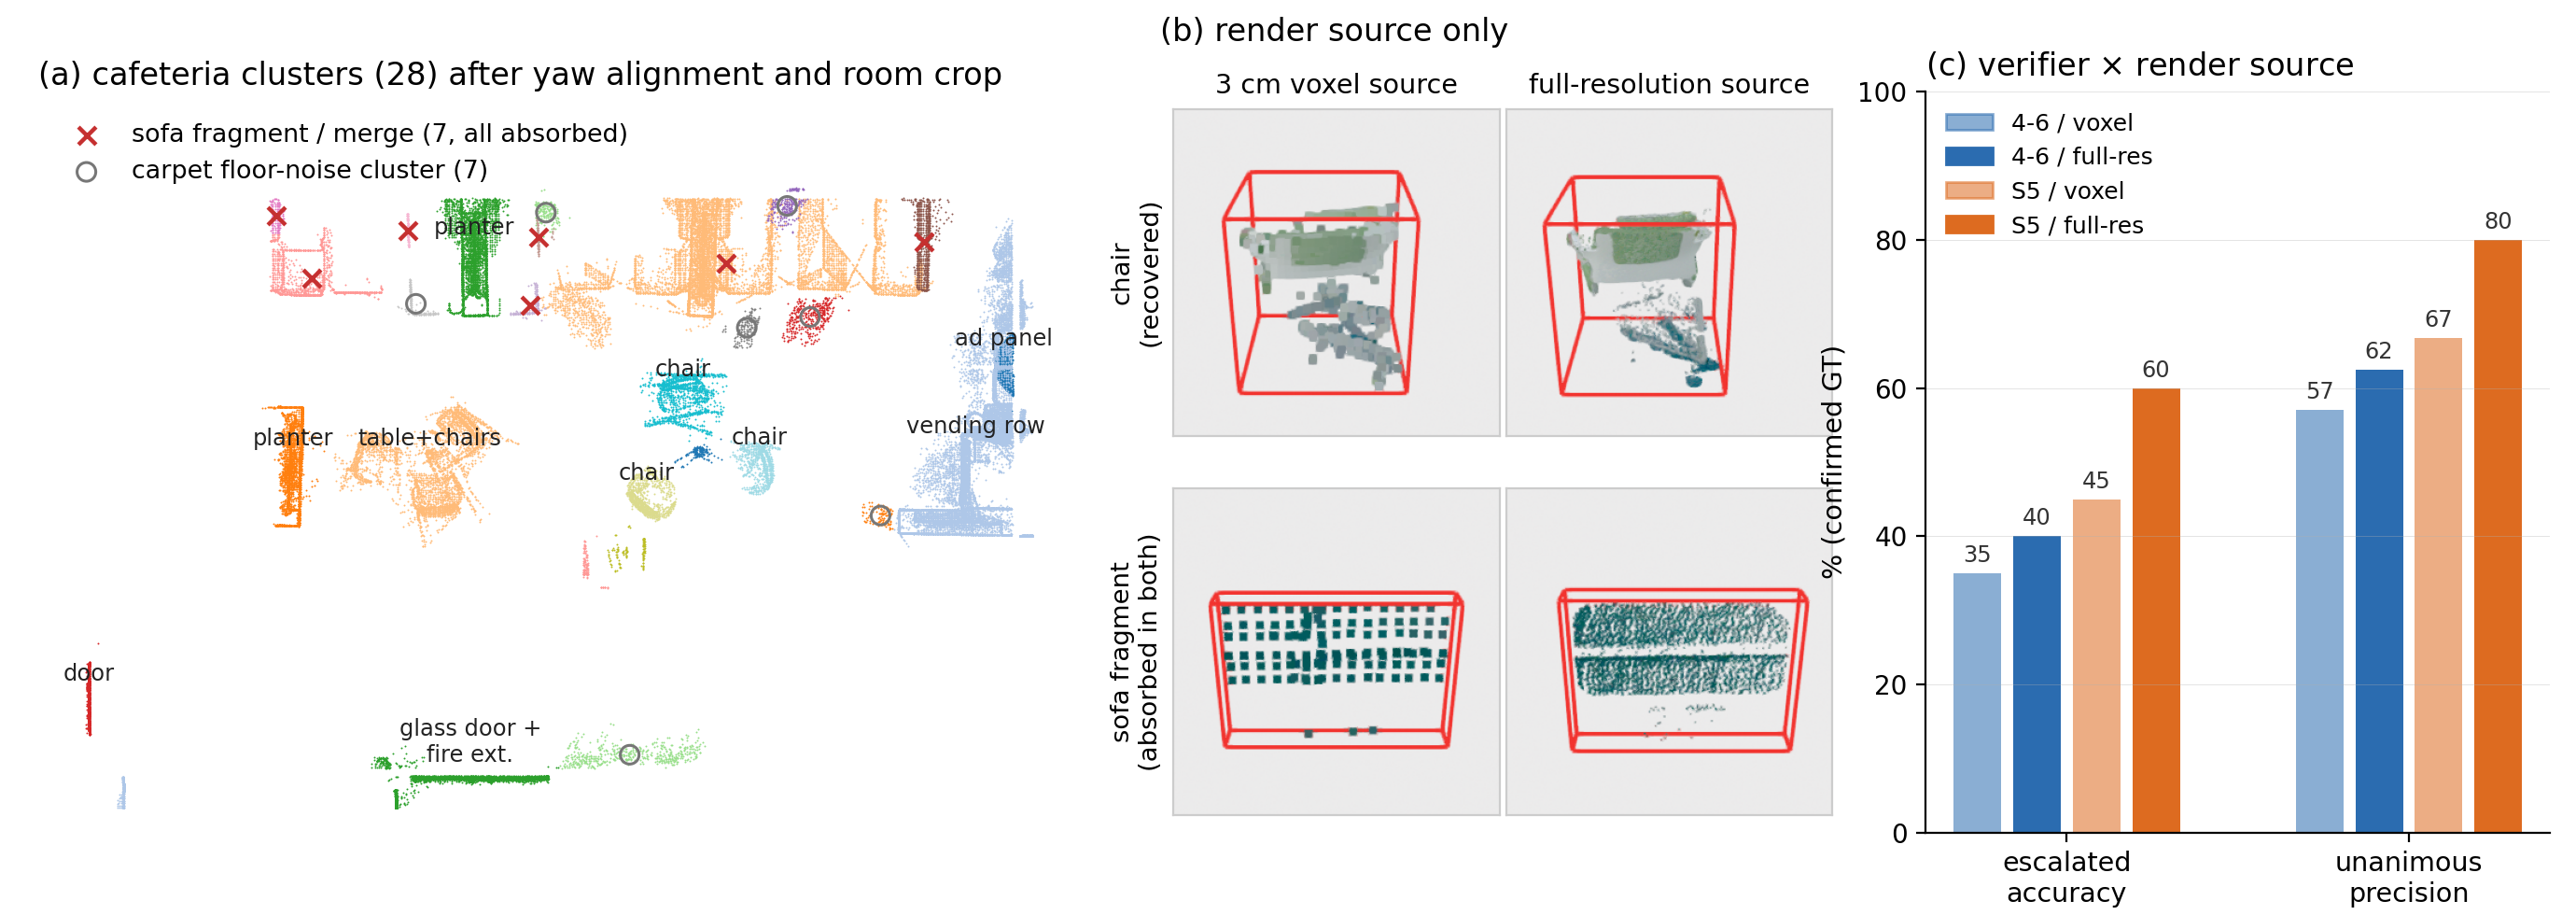
\includegraphics[width=\linewidth]{fig17_cafe_stress.png}
\caption{Cafeteria stress scene. (a)~The 28 clusters after automatic
yaw alignment and room crop; crosses mark the seven sofa
fragments/merges (absorbed as \texttt{clutter} in every condition of
Table~\ref{tab:cafe}), circles the seven carpet floor-noise clusters.
(b)~One cluster, rendered from the 3\,cm working cloud (left) and from
full-resolution re-associated points (right) under the identical
512-px protocol: the chair (top) is recovered by the render-source
change alone; the sofa fragment (bottom) is not. (c)~Escalated
accuracy (confirmed GT, $n{=}20$ per cell) and unanimous precision
(per-bar $n=8$--$15$ unanimous objects, annotated on each bar) across
verifier $\times$ render source; error bars are 95\% Wilson intervals,
wide on the precision bars because unanimous sets are small---the
point estimates order the cells, the intervals bound how far.}
\label{fig:cafe}
\end{figure}

\paragraph{Cross-floor stress scene.}
The cafeteria scene (Sec.~\ref{sec:setup}) probes the same protocol on
a furnishing domain the campaign never saw: carpeted floor, fabric sofa
booths, planter partitions (Fig.~\ref{fig:cafe}a). The backbone
transfers mechanically---57M points to 28 clusters in 13.5\,s after an
automatic wall-normal yaw alignment---but verification does not
(Table~\ref{tab:cafe}, first row): escalated accuracy reaches only
35\% against confirmed owner GT, and unanimous precision falls to
57.1\%, with two unanimous keyboard phantoms on carpet-noise clusters
and a chair unanimously absorbed as \texttt{clutter} (a fourth
unanimous miss, a table pedestal, falls on plausible-graded GT). The
errors are structured, not diffuse. The scene's
dominant object family---the sofas---enters the pipeline pre-broken,
split into five cushion fragments and two sofa--table merges, and every
one is absorbed (crosses in Fig.~\ref{fig:cafe}a); carpet pile leaves
seven residual floor-noise clusters above the RANSAC floor plane
(circles; the floor-material analogue of the ceiling remnants of
Sec.~\ref{sec:exp-seg}); and the confidence gate quarantines 9 of the
16 wrong labels over the 25 scored clusters as unverified while the
unanimous errors pass.

\paragraph{Render source $\times$ verifier.}
Two upgrades are then applied factorially (Table~\ref{tab:cafe},
Fig.~\ref{fig:cafe}c): re-rendering the identical 512-px view sets
from full-resolution re-associated points instead of the 3\,cm working
cloud (isolating render quality at unchanged protocol and cost,
$\sim$\$2.5/scene), and swapping the verifier for Sonnet~5. The two
levers act on different error classes. The render-source change
repairs \emph{whole-object} ambiguity for both verifiers: under
Sonnet~4-6 the keyboard phantoms vanish, both chairs recover
(including the unanimous miss; Fig.~\ref{fig:cafe}b, top), and both
doors resolve correctly, one via escalation---while the voxel renders
block the same chairs and doors under Sonnet~5 as well. The verifier
upgrade adds accuracy on top of whichever source it is given
(35$\rightarrow$45\% on voxel, 40$\rightarrow$60\% on full-resolution
sets): on this scene the newer model is uniformly better---in contrast
to its unanimous-precision loss on the industrial 512-px sets in the
upgrade check above---so even the \emph{sign} of a model upgrade is
domain-dependent. The render-source lever carries the same caveat: symmetric controls
that re-render \emph{both industrial scenes} from full-resolution
points reverse the effect---showroom escalated accuracy drops from
88.9\% to 80.6\% (base 77.8\%$\rightarrow$69.4\%; unanimous precision
holds at 100\%) and robot-hall from 84.4\% to 68.8\% (unanimous
precision 94.4\%$\rightarrow$83.3\%). The added texture invites
over-specific labels---a junction box read as a pipe assembly, the
wall TV as a ladder, clutter piles as keyboards, boxes, and trash
cans---where the coarser working-cloud render had left a correct
verdict, so the main campaign's voxel-source protocol stands as the
right default for the industrial scenes, and the cross-scene
comparison (first row of Table~\ref{tab:cafe} against
Table~\ref{tab:verification}) is same-protocol by construction. What
neither lever reaches is fragmentation: the seven sofa clusters are
absorbed in all four cells (Fig.~\ref{fig:cafe}b, bottom) and the
planters stay mislabeled.
Segmentation bounds what any verifier can see; render quality bounds
what a given verifier resolves; the model generation buys accuracy
only on top of both. Together with the upgrade check, the stress scene
fixes the reading of Table~\ref{tab:verification}: tier precision is a
scene- and domain-scoped measurement, to be re-estimated per
deployment---cheaply, via a small owner-confirmed probe set---rather
than a property of the architecture.

\paragraph{Segmentation parameters.}
The backbone's parameter sensitivity (36-combination sweep) and the
conditional refinement rules are ablated where their context lives, in
Sec.~\ref{sec:exp-seg}.

\paragraph{Voxel resolution and registration noise.}
Two controlled perturbations of the robot-hall backbone, scored per
object against the owner-grounded reference of
Sec.~\ref{sec:exp-seg}, bound the geometric operating regime. Voxel
size is not a free knob but part of a jointly calibrated triple with
$(\varepsilon, \mathrm{min\_points})$: at the baseline 3\,cm the full
backbone recovers 42/42 reference objects, but refining to 2\,cm
collapses recall to 0.36 (density rises, the fixed
$\varepsilon{=}0.30$ bridges gaps, 22 objects merge) and coarsening to
5\,cm collapses it to 0.33 (small objects starve below the 100-point
floor, 18 misses)---so the voxel size must be reported with the
clustering parameters, as Table~\ref{tab:sampleflow}'s pipeline
configuration does. Seeded per-point Gaussian noise applied to the raw
cloud before the backbone probes registration error at the point
level: at $\sigma{=}5$\,mm---the scale of the scanner's real per-scan
bundle error (4--5\,mm)---recall drops to 0.48, and by
$\sigma{=}20$\,mm (4$\times$ bundle error) the backbone effectively
fails (0.07), the dominant mechanism being saturation of the 5\,cm
RANSAC inlier band: un-removed wall residue grows from 267K to 853K
points and chains objects into merged clusters (39/42 merged) rather
than fragmenting them. We note the regime carefully: per-point scatter
at these levels is an artificial stress---the real $\sim$5\,cm
inter-epoch ICP residual is a rigid-transform error the pipeline
absorbs at the KG matching level (Sec.~\ref{sec:exp-update}), not
per-point noise---so the practical claim is robustness at the real
bundle-error scale, contingent on the structure-removal stage, which
is the first component to saturate. Color variation is not isolated by
any experiment in this paper: the render-source ablation above changes
point density and silhouette detail together with color, so it is an
appearance-quality control rather than a pure photometric one, and a
color-only perturbation study remains open.

\section{Application Demonstrations}
\label{sec:applications}

This section demonstrates the framework in use. The semantic mission
experiment of Sec.~\ref{sec:semnav} is quantitative; the twin injection
of Sec.~\ref{sec:twin} illustrates the single-store integration surface;
and Sec.~\ref{sec:realrobot} repeats the mission interface on the
physical AMMR, with the console, the twin, and the robot all served from
the same knowledge graph.

\subsection{Semantic Mission Execution in Simulation}
\label{sec:semnav}

We close the loop from scan-derived knowledge to autonomous behavior. The
TOSM robot layer is instantiated from the platform's URDF and navigation
configuration (footprint, drive type, sensor mounts, velocity limits) and
ingested alongside objects and places, completing the three-element TOSM
model. A \emph{semantic mediator} resolves natural mission commands ---
\texttt{goto\_place}, \texttt{goto\_object}, \texttt{patrol},
\texttt{return\_home} --- against the knowledge graph: places resolve to
free-space points at region centroids, objects to approach poses computed
from the target's footprint and the robot's radius---the kinematics-aware
resolution style of TOSMNav~\cite{joo2022fsom}, which checks robot
footprints against doorway entrance sizes in its planning rules---with
the verification gate deciding eligibility. The mediator covers command
resolution only; full hierarchical task planning over the same TOSM
knowledge (PDDL/POPF in~\cite{joo2022fsom}) is the natural next consumer
of the graph and is out of scope here. A hybrid deliberative/reactive behavior
tree~\cite{colledanchise2018bt,iovino2022btsurvey}
(Fig.~\ref{fig:bttree}) executes the resolved goals through
Nav2~\cite{macenski2020marathon}, with a
reactive layer that preempts the mission on low battery or an interrupt
and returns the robot to its home pose. The management console
(Sec.~\ref{sec:overview}) issues commands and edits the graph live; the
mediator hot-reloads owner edits, so refuting a phantom in the UI changes
robot behavior on the next command without a restart.

Experiments run in a Gazebo~\cite{koenig2004gazebo} world generated from
the same exploration
occupancy grid that anchors the place layer, so world, navigation map, and
knowledge graph share one frame. The simulated vehicle is a digital proxy
of the target platform itself: the AMMR's footprint
($1.25\times0.8$\,m), lidar mount, and velocity limits from the robot
layer are instantiated in the world, and the mediator derives approach
poses and clearance checks from the same layer (circumscribed radius
$0.74$\,m) --- the knowledge that \emph{describes} the robot is the
knowledge that \emph{drives} it. Mission-level metrics: over three
repetitions of a three-mission battery (approach the TV, go to the
seating area, return home), task success is 9/9, with mean leg path
lengths $4.6/5.4/1.8$\,m and completion times $16.5/24.9/15.0$\,s;
semantic resolution latency (command to accepted or refused goal) is
under one second, and a gate refusal stops the robot safely with zero
motion. The reactive layer supplies the safety-stop behavior: a
low-battery event during navigation preempts the active Nav2 goal and
returns the platform to a holding position at home, resuming only on
recovery. The phantom experiment (Table~\ref{tab:semnav})
sends the robot to three owner-refuted phantoms under two knowledge
states. Against the pre-feedback graph, all three phantoms carry
\emph{verified} labels, so the confidence gate passes them --- and the
waste takes three distinct forms: a pointless drive to a fluorescent
lamp; a \emph{false arrival} at a $7.4$\,m ``staircase'' whose approach
ring encloses the robot's own position, so the mission reports success at
a structure that does not exist; and $22$\,s of futile replanning toward
a wall-pillar ``book'' whose approach pose the platform's footprint
cannot reach at all. Against the graph after structure filtering and
owner feedback, the same commands are refused in about one second with
zero motion. Verification gating alone cannot stop verified phantoms; it
is the combination of gating, structure-noise removal, and owner
feedback that reduces the robot's exposure to unverified and phantom
semantic claims. Fig.~\ref{fig:semnav}
shows a gated mission trajectory and an ungated phantom drive.

\begin{table}[t]
\caption{Phantom-goal mission waste in simulation (AMMR proxy). The same
three commands are resolved against the knowledge graph before and after
structure filtering + owner feedback (both with the verification gate
active). Wasted path includes the return leg.}
\label{tab:semnav}
\footnotesize
\begin{tabular}{@{}llccc@{}}
\toprule
\textbf{KG state} & \textbf{Phantom target (truth)} & \textbf{Outcome} &
\textbf{Wasted path} & \textbf{Wasted time} \\
\midrule
pre-feedback & keyboard (fluorescent lamp) & driven & 1.7\,m & 16.8\,s \\
pre-feedback & staircase (bare wall) & false arrival & 0.6\,m & 5.7\,s \\
pre-feedback & book (wall pillar) & unreachable, aborted & 0\,m & 22.2\,s \\
\midrule
filtered + owner feedback & all three & refused & 0\,m & $\sim$1\,s \\
\bottomrule
\end{tabular}
\end{table}

\begin{figure}[t]
\centering
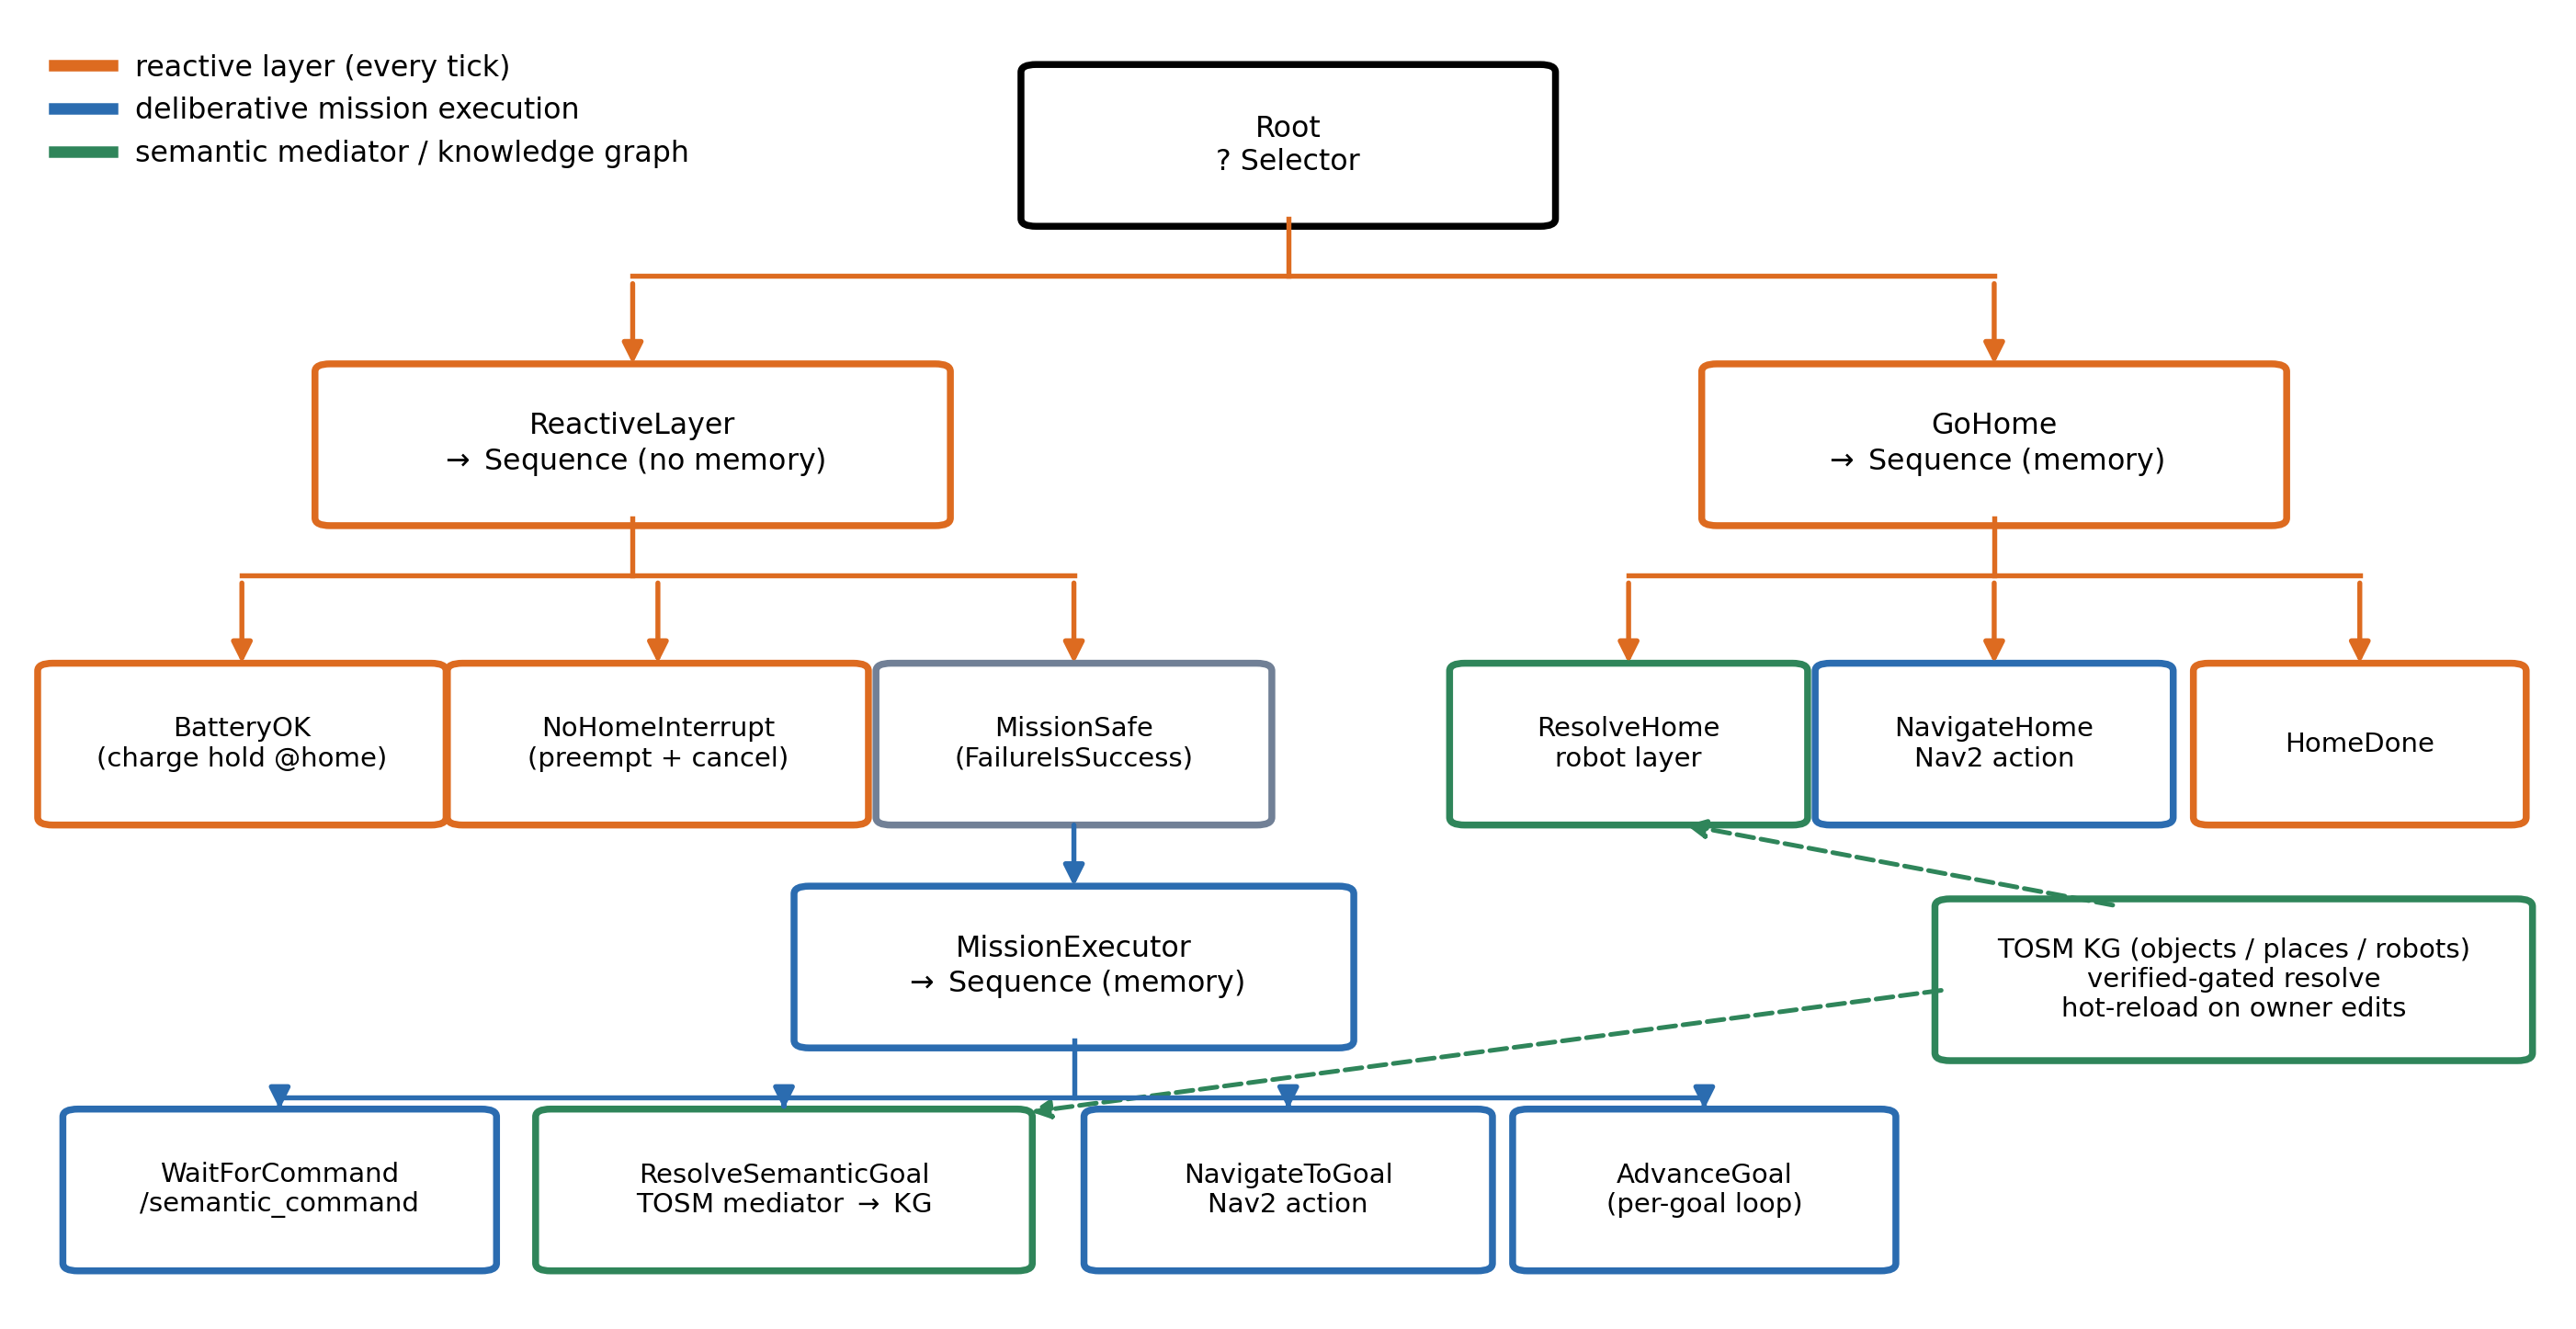
\includegraphics[width=0.9\linewidth]{fig16_bt_tree.png}
\caption{Hybrid deliberative/reactive mission behavior tree. The reactive
layer re-evaluates battery and interrupt conditions every tick and can
preempt navigation (canceling the active Nav2 goal); the deliberative
branch resolves semantic commands through the TOSM mediator, which
hot-reloads the knowledge graph when the management console edits it.
Highlighted nodes (violet) are the decisions the verified knowledge
graph drives: the semantic-resolve node, where a gated graph refuses
phantom or unverified goals, and the navigation node that consumes the
resolved pose; the unhighlighted reactive nodes are generic
behavior-tree machinery.}
\label{fig:bttree}
\end{figure}

\begin{figure}[t]
\centering
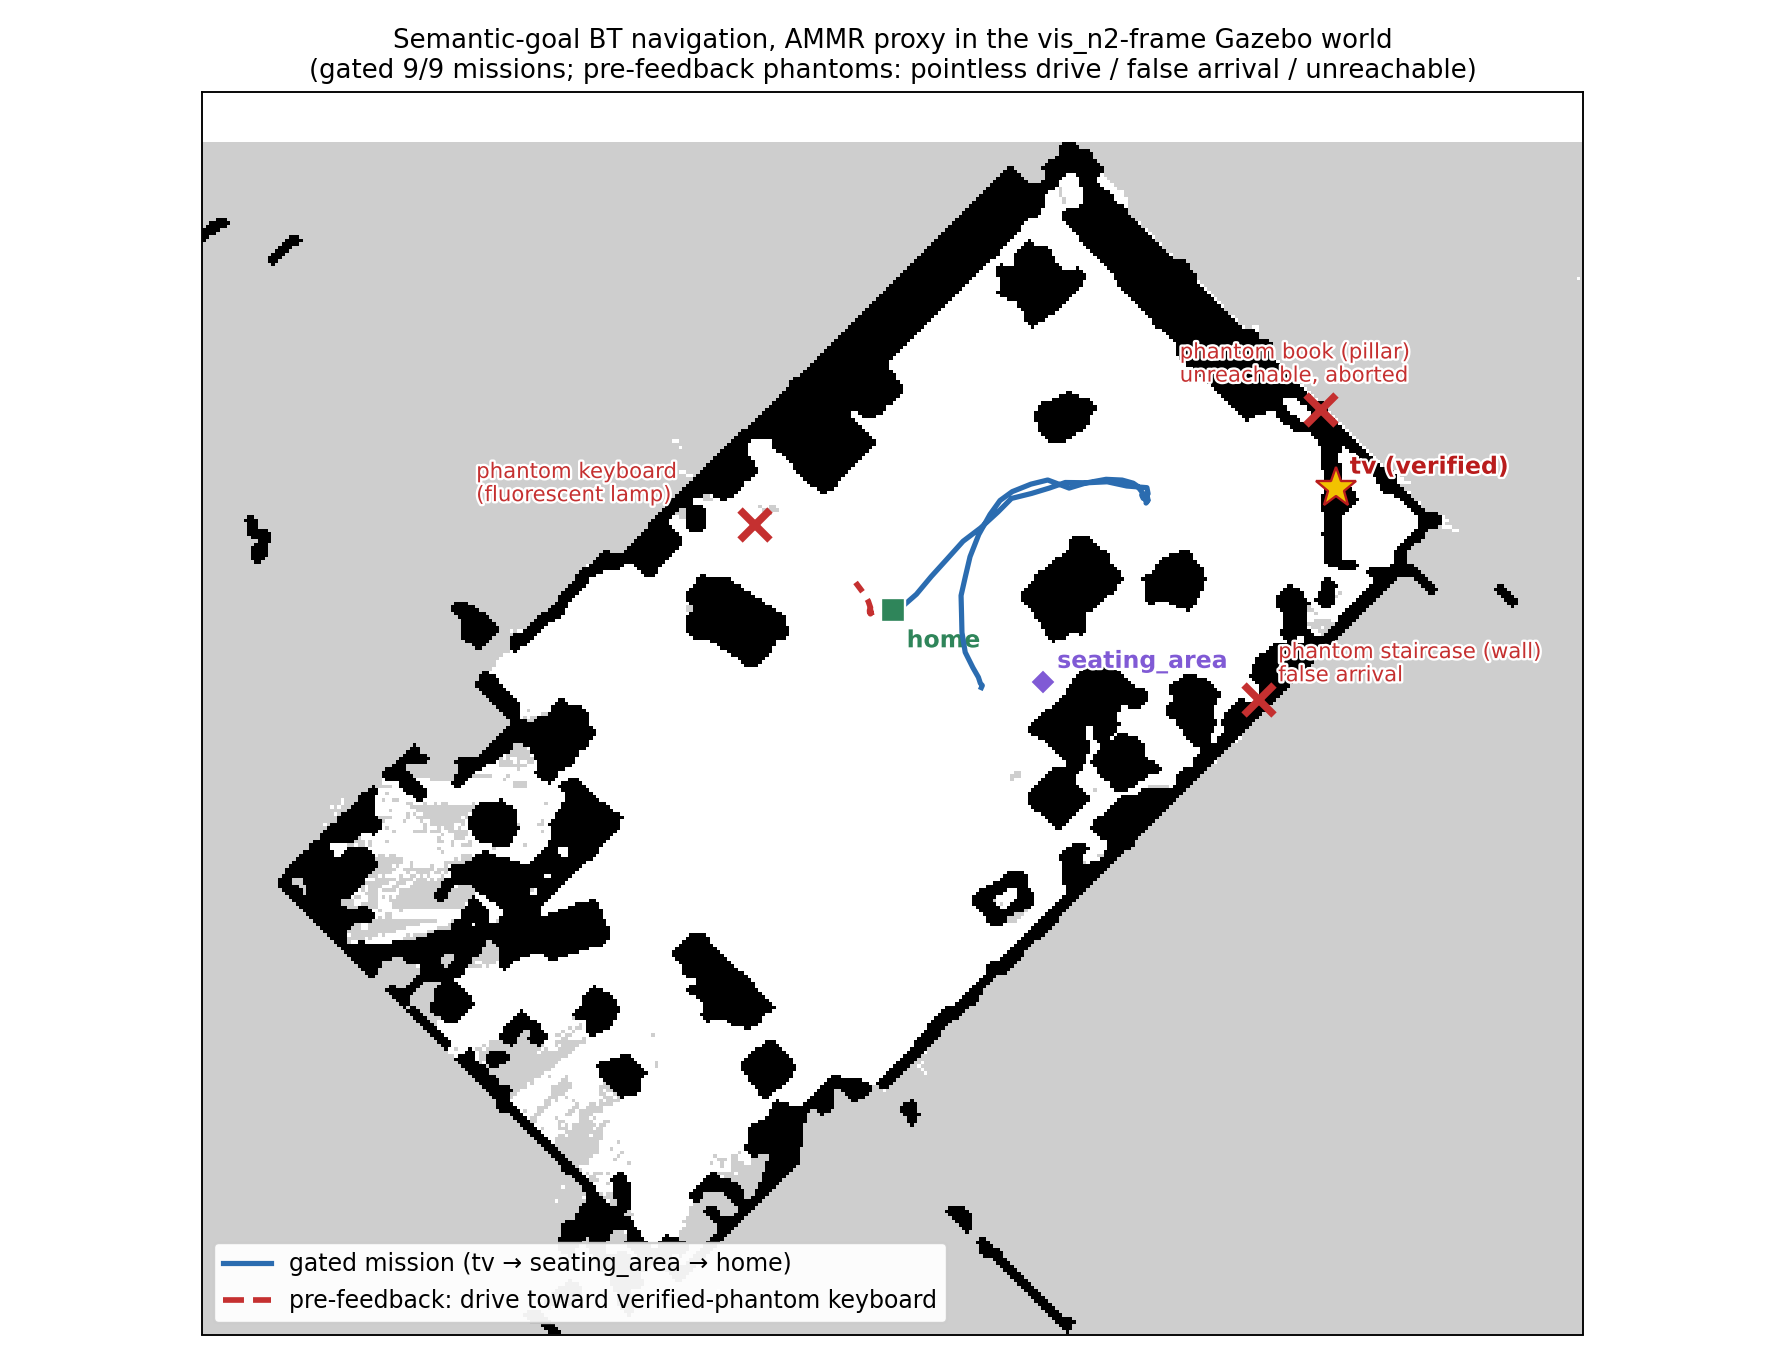
\includegraphics[width=0.8\linewidth]{fig15_semantic_nav_run.png}
\caption{Semantic-goal navigation of the AMMR proxy in the Gazebo twin of
the test room (world, map, and knowledge graph share the
exploration-scan frame). Blue: a gated three-mission run (TV
$\rightarrow$ seating area $\rightarrow$ home). Red dashed: against the
pre-feedback graph the robot drives toward a verified-phantom keyboard
--- a fluorescent lamp; crosses mark the three phantom goals with their
failure modes (pointless drive, false arrival, unreachable). All three
are refused once structure filtering and owner feedback are applied.
These runs establish the knowledge-graph--to--mission interface in a
physics simulation; Sec.~\ref{sec:realrobot} repeats the interface on
the physical platform.}
\label{fig:semnav}
\end{figure}

\subsection{Simulation Twin Injection}
\label{sec:twin}
Because every node carries an explicit model in the scan frame, the graph
injects directly into a physics simulation. We reuse the digital-twin
construction of our prior work~\cite{raaicon2026} and add the semantic layer:
each verified object spawns a labeled proxy (extent box or segmented cloud)
in NVIDIA Isaac Sim, with verification status, provenance, height level,
and label stability exposed in the scene inspector. Unverified objects
spawn as neutral gray placeholders---the gate is visible in the twin.
The knowledge graph is the \emph{single} semantic store: the management
console and the mission mediator read the same file live, and the Isaac
stage is re-derived from it (in the shared map frame) whenever the graph
changes, so an owner edit propagates to the robot's next goal, the
console, and the twin from one write. The discipline is
self-auditing --- deriving the stage from the graph immediately
\emph{visualized} eighteen stale earlier-epoch nodes as orphan boxes that
per-view export paths had silently hidden, prompting the cleanup revision
of Sec.~\ref{sec:exp-update}.

\subsection{Real-Robot Mission Execution}
\label{sec:realrobot}
To close the loop on hardware, the mission stack of Sec.~\ref{sec:semnav}
was run unchanged against the physical AMMR in the test room (the robot
hall configuration), with the knowledge graph of
Sec.~\ref{sec:exp-update} as the semantic store. The platform runs its own
localization and Nav2 stack on an independently built occupancy map; a
thin bridge node replaces the simulator: it converts the robot's
localization pose into the scan frame through a single SE(2) offset,
calibrated once by parking the robot on a taped start spot of known scan
coordinates, and forwards the mediator's resolved goals (scan frame) to
the robot's on-board navigation in the robot's map frame. Nothing above
the bridge changes: commands are issued from the management console, the
mediator resolves and gates them against the graph, the behavior tree
executes them, and the Isaac Sim twin mirrors the robot from the same
store. Fig.~\ref{fig:realrobot} shows two filmed missions and
Table~\ref{tab:realrobot} summarizes all runs; Video~S1 contains the
synchronized console, twin, and camera footage.

Three semantic drives completed --- two \texttt{goto\_object} approaches
to the wall TV and one \texttt{goto\_place} drive into the monitor
workstation region, each $3.6$--$4.0$\,m from the start --- in $14$--$22$\,s
with arrival errors of $0.22$--$0.34$\,m (mean $0.30$\,m) between the
robot's localized pose and the resolved goal; a place command issued
while the robot already stood inside the region completed without motion
($0.11$\,m from the region goal). The gate behaved as in simulation:
\texttt{goto\_object keyboard}, the owner-refuted phantom of
Table~\ref{tab:semnav}, was refused by the mediator in under one second
with zero robot motion, twice. Missions were issued one at a time from
a standing start. The exercise is a bounded validation --- one room, one
platform, three completed drives --- but it confirms that the graph that
survives verification, gating, and owner feedback is directly consumable
by a real robot, and that the twin, console, and robot stay consistent
because they read one store.

\begin{table}[t]
\caption{Real-robot semantic missions on the AMMR (test room,
15~Sep~2026). Goals are resolved by the mediator in the scan frame;
distance is straight-line start-to-goal; arrival error is the
localized-pose--to--goal distance at mission completion.}
\label{tab:realrobot}
\begin{adjustwidth}{-\extralength}{0cm}
\centering
\scriptsize
\setlength{\tabcolsep}{3.5pt}
\begin{tabular}{@{}llcccl@{}}
\toprule
\textbf{Command} & \textbf{Resolved goal (m)} & \textbf{Dist.} & \textbf{Time} & \textbf{Err.} & \textbf{Outcome} \\
\midrule
\texttt{goto\_object tv} & tv\_006 approach (3.09, 1.91) & 4.0\,m & 14\,s & 0.34\,m & completed \\
\texttt{goto\_object tv} (Fig.~\ref{fig:realrobot}a) & tv\_006 approach (3.09, 1.91) & 3.6\,m & 20.8\,s & 0.33\,m & completed \\
\texttt{goto\_place electrical\_maintenance\_area} (Fig.~\ref{fig:realrobot}b) & region ($-$0.69, 3.81) & 3.9\,m & 22.1\,s & 0.22\,m & completed \\
\texttt{goto\_place display\_briefing\_area} & region (3.31, 1.76) & 0.1\,m & $<$1\,s & 0.11\,m & completed (already inside) \\
\texttt{goto\_object keyboard} ($\times$2, phantom) & --- & --- & $<$1\,s & --- & refused by gate, no motion \\
\bottomrule
\end{tabular}
\end{adjustwidth}
\end{table}

\begin{figure}[t]
\centering
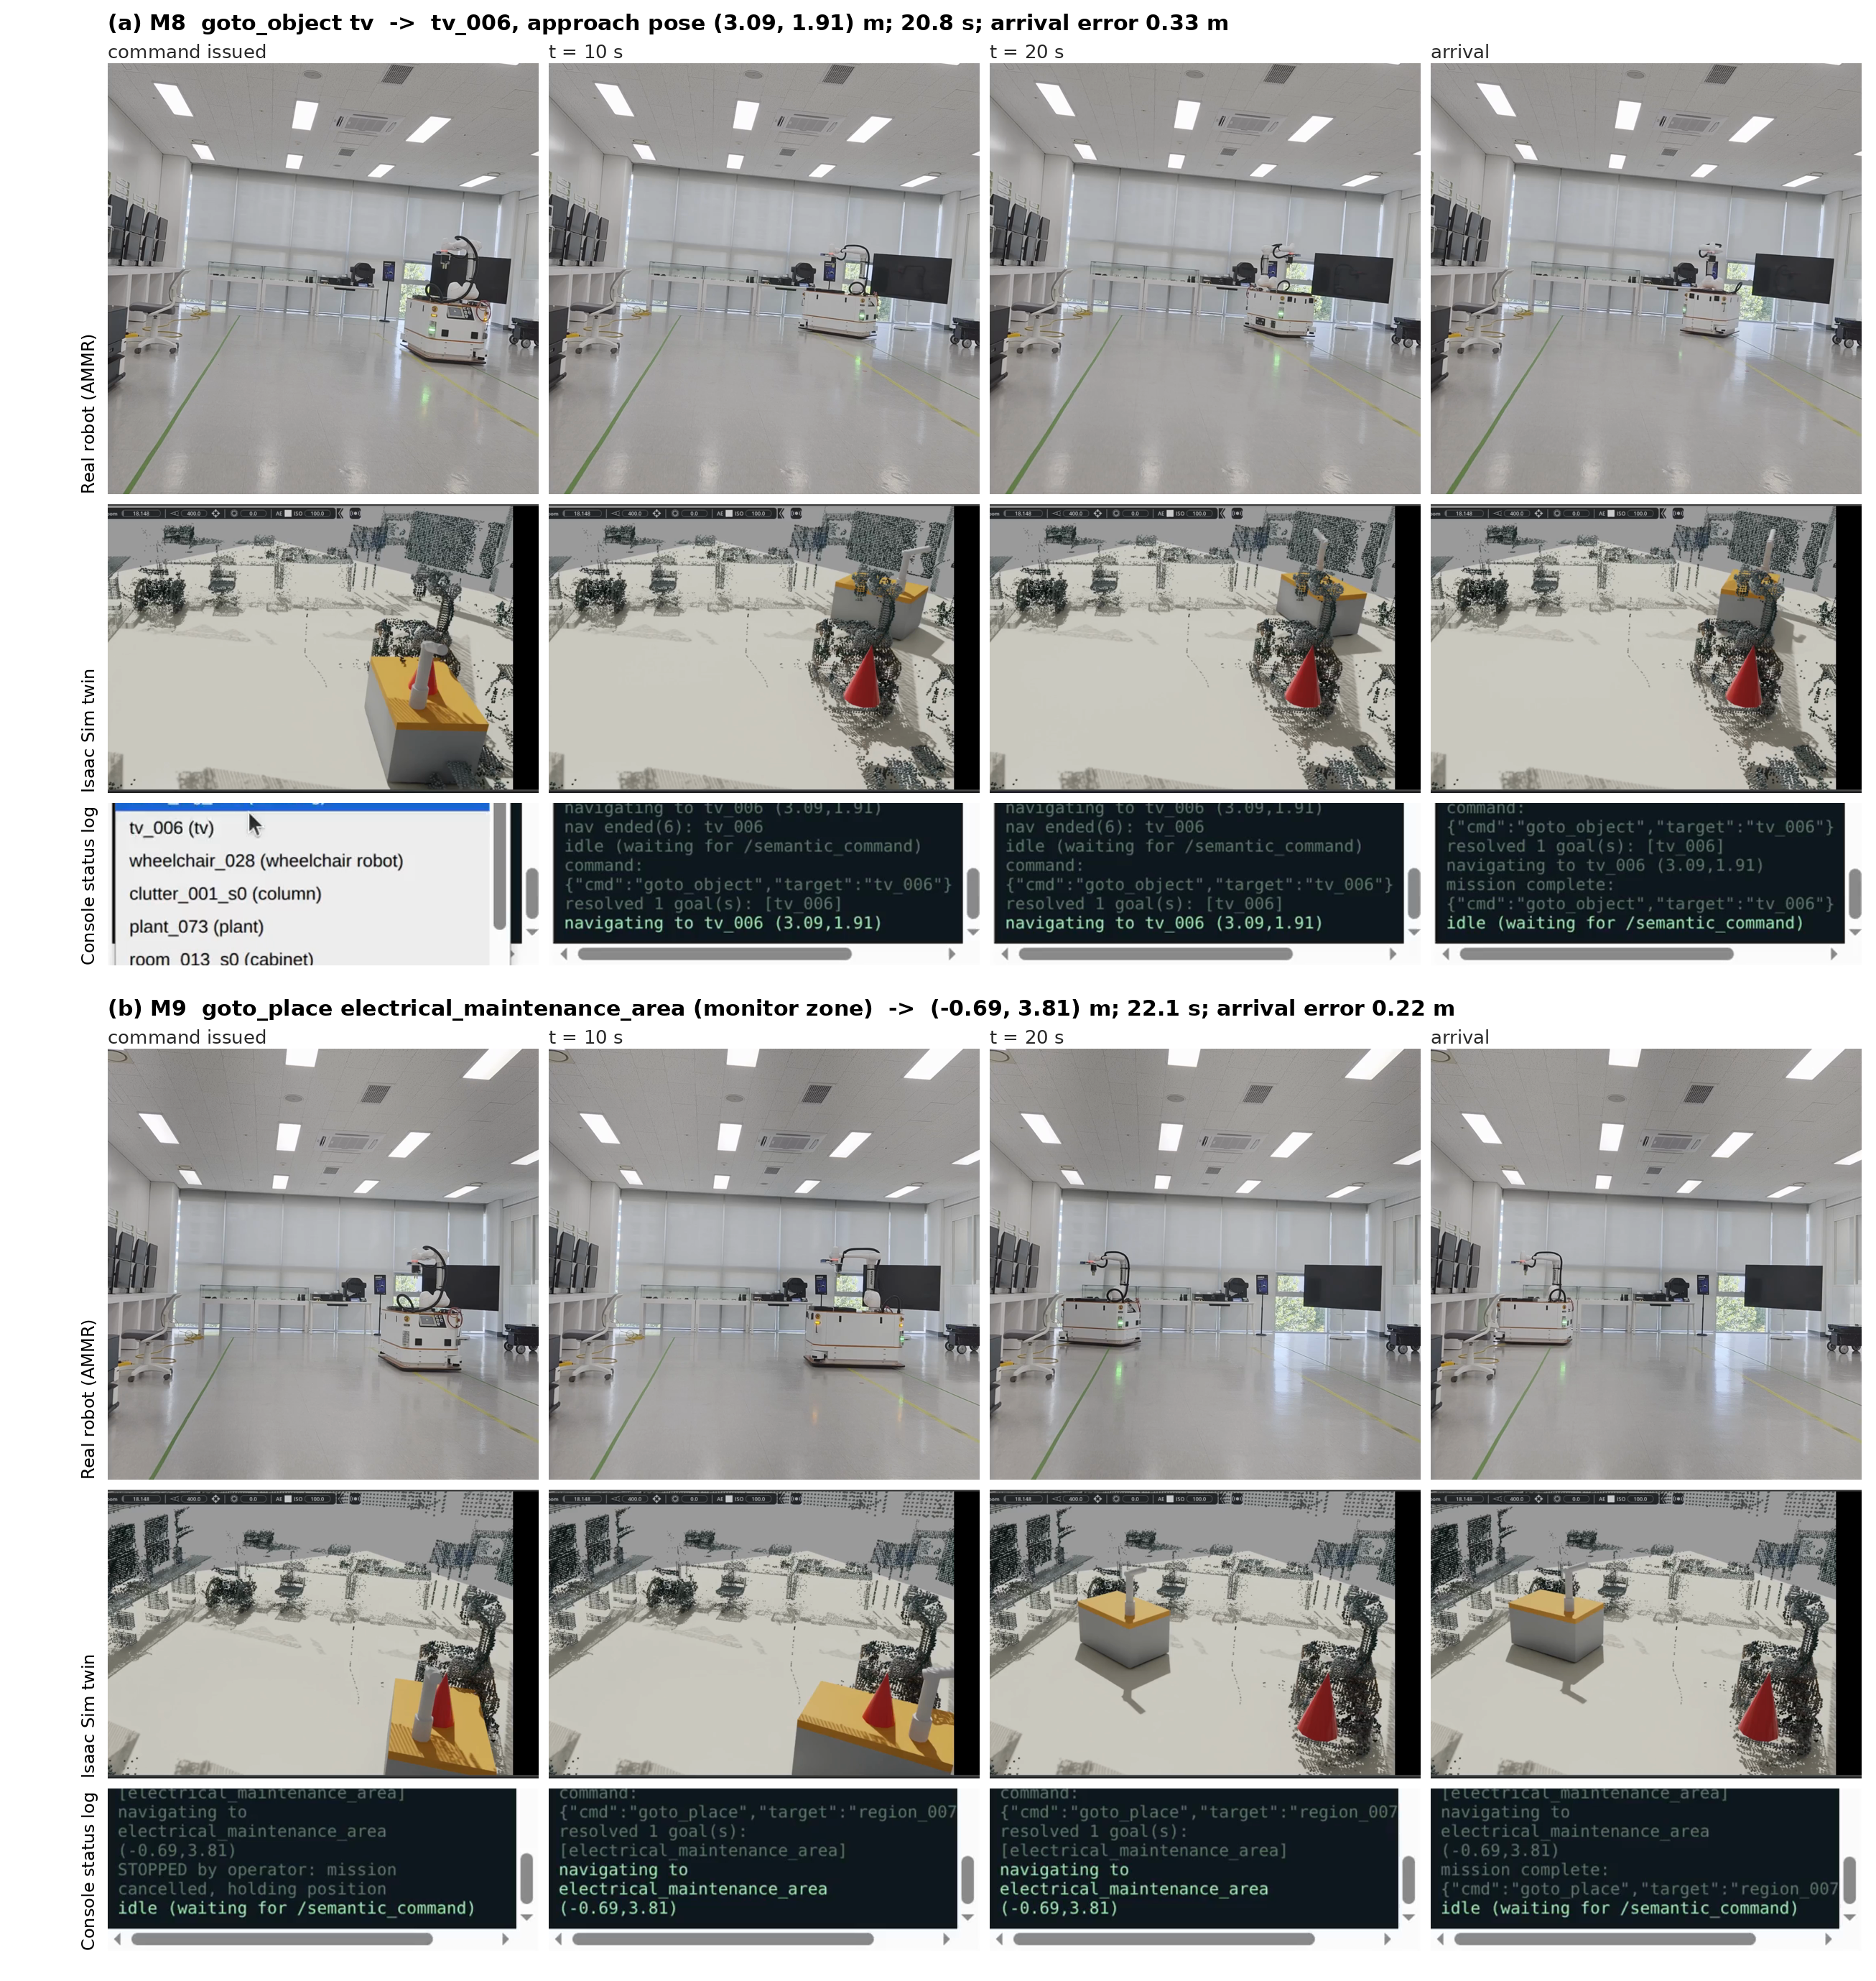
\includegraphics[width=\linewidth]{fig20_real_robot_missions.png}
\caption{Real-robot semantic missions (Table~\ref{tab:realrobot}). Rows:
the physical AMMR, the Isaac Sim twin derived from the same knowledge
graph (the red cone marks the twin's goal handle), and the management
console's status log; columns: command issued, $10$\,s, $20$\,s, and
arrival. (a)~\texttt{goto\_object tv}: the mediator resolves the
verified node \texttt{tv\_006} to an approach pose and the robot arrives
$0.33$\,m from it in $20.8$\,s. (b)~\texttt{goto\_place
electrical\_maintenance\_area}: the region containing the monitor
workstation, reached in $22.1$\,s with $0.22$\,m error. Video~S1 shows
the synchronized footage.}
\label{fig:realrobot}
\end{figure}

\section{Discussion}
\label{sec:discussion}

\paragraph{Cost and latency.}
VLM verification is the only paid stage. Escalation is bounded by its
trigger rate (51--58\% of objects), and per-call cost is $\sim$\$0.009;
full verification averages $\sim$\$0.09 per object (\$3.63 for a 38-cluster
run and \$7.37 for an 86-cluster run, all calls included). The incremental
design changes
the cost model qualitatively: a repeat scan costs \$0 (hash carry-over) and
a changed scene costs in proportion to its change (3.1\% of rebuild in our
measurement). Verification is offline; no VLM call sits on a robot's control
path.

\paragraph{Residual unverified content.}
On exploration-quality scans, 24\% of objects remain unverified (47\% on the
manual scan; 43\% on the 1/6-coverage ablation)---scan quality is the
dominant driver of verification yield. The framework's position is to expose
this residue, not shrink it cosmetically: unverified nodes stay queryable
with demoted types, and the gate is only as good as the verifier
(Sec.~5.3's unanimous-but-wrong cases; the escalated-verified keyboard trap
that survives gating on the robot hall). Verifier-bounded gating is a
property users must design around, and we report it as such.

\paragraph{Small low-reflectance objects.}
The clutter-absorption error class---disassembled robot, poster stand, and
the controlled-change floor circulator all verified as
\texttt{clutter}---shows a systematic blind spot: geometrically detected,
semantically flattened. Change detection still works (the circulator was
correctly inserted), but type-level recall for small dark appliances needs
either close-range imagery or targeted re-rendering.

\paragraph{Structure remnants.}
The soffit filter removes vertical transition bands, but horizontal and
sloped ceiling patches and content seen through openings survive structure
removal (six residual cases in the robot hall). These are bounded,
enumerable artifacts; extending the filter to non-vertical remnants is
mechanical future work.

\paragraph{The coverage paradox.}
Better scans can make density-based decomposition worse: at 99.6\% coverage,
gaps between adjacent objects close and DBSCAN chains 41\% of the scene into
one mega-cluster. Our measurements show this artifact accounts for only
$\sim$12\% of the epoch's absent nodes (5/43 recoverable by tighter
re-splitting; 4/43 by Point-SAM refinement)---the rest is genuine change---but
the effect argues for coverage-adaptive clustering or learned instance
priors as the backbone's next iteration, applied under the same
flagged-candidate discipline as our Point-SAM rule.

\paragraph{Scope.}
Results come from one scanner, one building, and object-level change;
structural change (walls, large fixtures) and cross-site generalization are
untested. The three-epoch study mitigates but does not remove the two-scene
limitation. The place layer's regions are parameterized SLIC superpixels over the grid
map: spatial cells rather than architecturally meaningful rooms, with the
superpixel count fixed by hand; inferring wall- and doorway-aligned region
boundaries is future work.

\section{Conclusion}
\label{sec:conclusion}

We presented TLS-SMF, a framework that turns registered terrestrial laser scans into
a queryable, confidence-aware, and maintainable semantic knowledge graph for
indoor robots. A deterministic geometric backbone makes decomposition
reproducible and diffs meaningful; multi-view VLM verification with automatic
escalation attaches calibrated trust to every label while retaining what it
cannot resolve as explicitly unverified; and mint-once identities with
two-pass matching turn re-scans into node-level upserts whose cost scales
with actual change. Across two industrial scenes and a real three-epoch
study of one room, the framework improved verification accuracy by up to 11
points through escalation, blocked hallucination traps by gating the data
rather than instructing the model, preserved object identity across three
scan epochs including a controlled physical change, and re-verified repeat
scans at zero marginal VLM cost.

Future work follows the limitations surfaced by our own evaluation:
extending the remnant filter to non-vertical structure artifacts,
coverage-adaptive decomposition to resolve the mega-cluster paradox,
close-range or re-rendered imagery for small low-reflectance objects,
structural-change updating beyond the object level, automatic place
segmentation to close the loop with the DK-SMF lineage, and embodied
validation in which a robot plans against the graph---including its
unverified residue---in the loop.


\bibliographystyle{unsrt}
\bibliography{refs}

\end{document}
